%--------------------------------------
%appel de la classe de document et de ses options
%--------------------------------------

\documentclass[a4paper, 11pt, twoside, fleqn]{memoir}

\usepackage{AOCDTF}

\addbibresource{../../bibliographies/chimie.bib} %à redéfinir une fois le cours entamé le chemin ne sera pas le même selon les cours !
\addbibresource{../../bibliographies/sciences_naturelles.bib} %à redéfinir une fois le cours entamé le chemin ne sera pas le même selon les cours !
\addbibresource{../../bibliographies/electrotechnique.bib} %à redéfinir une fois le cours entamé le chemin ne sera pas le même selon les cours !

%--------------------------------------
%données du document
%--------------------------------------

\formationtrue %si \formationfalse alors l'intitulé de la formation n'apparait pas sur la page de titre

\corpsdemetier{Métiers des technologies associées}
\siglemetier{MTA}
\nombreauteur{1}

\formation{BTS \'Electrotechnique}
\matiere{Physique-chimie}
\cours{Pré-requis}

\auteura{Bruno}{Douchy}
\siglemetierauteura{MTA}
\auteurb{}{}
\siglemetierauteurb{nul}
\auteurc{}{}
\siglemetierauteurc{nul}
\auteurd{}{}
\siglemetierauteurd{nul}

\typemedia{paper} %choix screen ou paper pour les vidéos et schémas animés

\decoupagechapitre{5} %espacement des marqueurs entre les différents chapitres (à régler en fin de rédaction) (5cm vaut un espacement équivalement à la hauteur du marqueur, une page ne peut en contenir que 5 avec cet espacement-la mais il est le plus équilibré)

%--------------------------------------
%corps du document
%--------------------------------------

\begin{document} %corps du document

%--------------------------------------
%préface, page de couverture, table des matières...
%--------------------------------------

\frontmatter

\Framefalse %défini la booléenne Frame comme faux

	%--------------------------------------
	%page de couverture et de titre
	%--------------------------------------

\pagecouverture
\pagetitre
\marqueurchapitre
\media{\thetypemedia}{}{
	\makeatletter
	\setboolean{@twoside}{false}
	\makeatother}
	
	\pagestyle{plain} %style de page avec en-tête et pied-de-page
	\pagenumbering{roman}
	\openany
	
	%--------------------------------------
	%listes de contenus
	%--------------------------------------
	
	{\hypersetup{linkcolor=black}\tableofcontents*} %table des matières en noir
	\newpage
	{\hypersetup{linkcolor=black}\listoftables*} %liste des tableaux en noir
	\newpage
	{\hypersetup{linkcolor=black}\listoffigures*} %liste des figures en noir
	{\hypersetup{linkcolor=black}\tcblistof[\chapter*]{frm}{Liste des formules}} %liste des équations en noir
	{\hypersetup{linkcolor=black}\tcblistof[\chapter*]{dfn}{Liste des définitions}} %liste des définitions en noir
	{\hypersetup{linkcolor=black}\tcblistof[\chapter*]{xmpl}{Liste des exemples}} %liste des définitions en noir

	\media{\thetypemedia}{\openright}{} %début de chapitre à "droite" mais comme demarrage de la numérotation inversé avec la page de titre, ça décale l'ouverture des chapitre à gauche

	%--------------------------------------
	%inclusion du chapitre d'introduction
	%--------------------------------------
	
	%utiliser les environnement \begin{comment} \end{comment} pour mettre en commentaire le préambule une fois la programmation appelée dans le document maître (!ne pas oublier de mettre en commentaire \end{document}!)

%--------------------------------------
%chap_0_preface
%--------------------------------------

\begin{comment}

\documentclass[a4paper, 11pt, twoside]{memoir}

\usepackage{AOCDTF}

%--------------------------------------
%CANEVAS
%--------------------------------------

\newcommand\BoxColor{\ifcase\thechapshift blue!30\or brown!30\or pink!30\or cyan!30\or green!30\or teal!30\or purple!30\or red!30\or olive!30\or orange!30\or lime!30\or gray!\or magenta!30\else yellow!30\fi} %définition de la couleur des marqueurs de chapitre

\newcounter{chapshift} %compteur de chapitre du marqueur de chapitre
\addtocounter{chapshift}{-1}
	
\newif\ifFrame %instruction conditionnelle pour les couleurs des pages
\Frametrue

\pagestyle{plain}

% the main command; the mandatory argument sets the color of the vertical box
\newcommand\ChapFrame{%
\AddEverypageHook{%
\ifFrame
\ifthenelse{\isodd{\value{page}}}
  {\backgroundsetup{contents={%
  \begin{tikzpicture}[overlay,remember picture]
  \node[
  	rounded corners=3pt,
    fill=\BoxColor,
    inner sep=0pt,
    rectangle,
    text width=1.5cm,
    text height=5.5cm,
    align=center,
    anchor=north west
  ] 
  at ($ (current page.north west) + (-0cm,-2*\thechapshift cm) $) %nombre négatif = espacement des marqueurs entre les différents chapitres (à régler en fin de rédaction) (4.5cm vaut un espacement équivalement à la hauteur du marqueur, une page peut en contenir 6 avec cet espacement-la mais il est le plus équilibré)
    {\rotatebox{90}{\hspace*{.5cm}%
      \parbox[c][1.2cm][t]{5cm}{%
        \raggedright\textcolor{black}{\sffamily\textbf{\leftmark}}}}};
  \end{tikzpicture}}}
  }
  {\backgroundsetup{contents={%
  \begin{tikzpicture}[overlay,remember picture]
  \node[
  	rounded corners=3pt,
    fill=\BoxColor,
    inner sep=0pt,
    rectangle,
    text width=1.5cm,
    text height=5.5cm,
    align=center,
    anchor=north east
  ] 
  at ($ (current page.north east) + (-0cm,-2*\thechapshift cm) $) %nombre négatif = espacement des marqueurs entre les différents chapitres (à régler en fin de rédaction) (4.5cm vaut un espacement équivalement à la hauteur du marqueur, une page peut en contenir 6 avec cet espacement-la mais il est le plus équilibré)
    {\rotatebox{90}{\hspace*{.5cm}%
      \parbox[c][1.2cm][t]{5cm}{%
        \raggedright\textcolor{black}{\sffamily\textbf{\leftmark}}}}};
  \end{tikzpicture}}}%
  }
  \BgMaterial%
  \fi%
}%
  \stepcounter{chapshift}
}

\renewcommand\chaptermark[1]{\markboth{\thechapter.~#1}{}} %redéfinition du marqueur de chapitre pour ne contenir que le titre du chapitre %à personnaliser selon le nombre de chapitre dans le cours

%--------------------------------------
%corps du document
%--------------------------------------

\begin{document} %corps du document
	\openleft %début de chapitre à gauche

\end{comment}

\chapter{Préface}

\section{Avant-propos}

Ces cours de physique -- chimie appliquées à l'électrotechnique sont à la disposition des étudiants BTS \'Electrotechnique pour appréhender les origines de l'énergie électrique et sa maitrise appliquée aux environnements professionnels. La compréhension de ces matières est indispensable pour saisir la nature un peu abstraite de l'énergie électrique que les détenteurs du BTS \'Electrotechnique se doivent de maitriser.\\
Ces cours sont la référence pédagogique pour toute la formation et ils regroupent toutes les connaissances théoriques à maitriser à l'issue de la formation. Il couvrira donc le programme initial et abordera également des notions de physique -- chimie supplémentaires, pour favoriser à l'étudiant sortant lors de son insertion professionnelle. Chaque fin de chapitre est composé d'un résumé de l'essentiel à retenir.\\

L'énergie électrique puise ses origines dans l'aspect chimique de la matière. Ce cours abordera donc des notions élémentaires de chimie atomique et quantique, qui sont des chapitres nécessaires pour comprendre le comportement des électrons, pourquoi tel ou tel élément est conducteur ou encore ce qu'on appelle un semi-conducteur.\\Tout ce qui sera abordé dans ce chapitre aura des répercussions dans les chapitres suivants de génie électrique et de physique -- chimie. Toutefois, comme les notions présentées pour ce cours de pré-requis de chimie sont issues de références de sciences techniques de l'ingénieur, leur maîtrise ne sera donc pas à exigée. Néanmoins, leur compréhension permettra de préparer judicieusement le terrain d'une éventuelle poursuite des études dans le secteur de l'électrotechnique.


\section{Références additionnelles et \textrm{\LaTeX}}

Ces cours n'ayant aucune prétention d'exhaustivité ni de savoirs innés, on retrouve en fin de document une bibliographie interactive compilant les références (livres, cours, sites internet\ldots) dont sont issues les informations contenues dans ce cours.\\Les liens de couleurs ~\textcolor{Blue}{\rule{1.5em}{1.2ex}}~ vous permettront d'accéder à ces documents contenus dans une base de données sur l'Intranet pour ceux en libre accès, ou de vous rediriger vers une libraire en ligne pour les quelques livres de références que nous vous conseillons d'investir.\\

La rédaction de ces documents est réalisée à partir d'un environnement de programmation \LaTeX. C'est un outil utilisé pour rédiger les livres, les publications scientifiques et universitaires ou encore les thèses de doctorats de façon normée.\\Il s'agit donc d'introduire cette nouvelle matière qui est enseignée dans les études supérieures des sciences techniques. Elle vous permettra autant de se familiariser avec un univers de programmation et ses mécanismes que de maitriser un outil de rédaction de document de qualité. Cela apportera un gain de crédibilité certain sortants lors de la rédaction de documents tels que le dossier du travail de réception ou les documents professionnels comme les lettres et les présentations.


%\end{document}
	
%--------------------------------------
%corps de texte, annexes
%--------------------------------------

\mainmatter

\Frametrue %défini la booléenne Frame comme vrai -> marqueurs de chapitre
	
	%--------------------------------------
	%inclusion des chapitres
	%--------------------------------------

	%utiliser les environnement \begin{comment} \end{comment} pour mettre en commentaire le préambule une fois la programmation appelée dans le document maître (!ne pas oublier de mettre en commentaire \end{document}!)

%--------------------------------------
%chap_1_chimie_atomique
%--------------------------------------

\begin{comment}

\documentclass[a4paper, 11pt, twoside]{memoir}

\usepackage{AOCDTF}

%--------------------------------------
%CANEVAS
%--------------------------------------

\newcommand\BoxColor{\ifcase\thechapshift blue!30\or brown!30\or pink!30\or cyan!30\or green!30\or teal!30\or purple!30\or red!30\or olive!30\or orange!30\or lime!30\or gray!\or magenta!30\else yellow!30\fi} %définition de la couleur des marqueurs de chapitre

\newcounter{chapshift} %compteur de chapitre du marqueur de chapitre
\addtocounter{chapshift}{-1}
	
\newif\ifFrame %instruction conditionnelle pour les couleurs des pages
\Frametrue

\pagestyle{plain}

% the main command; the mandatory argument sets the color of the vertical box
\newcommand\ChapFrame{%
\AddEverypageHook{%
\ifFrame
\ifthenelse{\isodd{\value{page}}}
  {\backgroundsetup{contents={%
  \begin{tikzpicture}[overlay,remember picture]
  \node[
  	rounded corners=3pt,
    fill=\BoxColor,
    inner sep=0pt,
    rectangle,
    text width=1.5cm,
    text height=5.5cm,
    align=center,
    anchor=north west
  ] 
  at ($ (current page.north west) + (-0cm,-2*\thechapshift cm) $) %nombre négatif = espacement des marqueurs entre les différents chapitres (à régler en fin de rédaction) (4.5cm vaut un espacement équivalement à la hauteur du marqueur, une page peut en contenir 6 avec cet espacement-la mais il est le plus équilibré)
    {\rotatebox{90}{\hspace*{.5cm}%
      \parbox[c][1.2cm][t]{5cm}{%
        \raggedright\textcolor{black}{\sffamily\textbf{\leftmark}}}}};
  \end{tikzpicture}}}
  }
  {\backgroundsetup{contents={%
  \begin{tikzpicture}[overlay,remember picture]
  \node[
  	rounded corners=3pt,
    fill=\BoxColor,
    inner sep=0pt,
    rectangle,
    text width=1.5cm,
    text height=5.5cm,
    align=center,
    anchor=north east
  ] 
  at ($ (current page.north east) + (-0cm,-2*\thechapshift cm) $) %nombre négatif = espacement des marqueurs entre les différents chapitres (à régler en fin de rédaction) (4.5cm vaut un espacement équivalement à la hauteur du marqueur, une page peut en contenir 6 avec cet espacement-la mais il est le plus équilibré)
    {\rotatebox{90}{\hspace*{.5cm}%
      \parbox[c][1.2cm][t]{5cm}{%
        \raggedright\textcolor{black}{\sffamily\textbf{\leftmark}}}}};
  \end{tikzpicture}}}%
  }
  \BgMaterial%
  \fi%
}%
  \stepcounter{chapshift}
}

\renewcommand\chaptermark[1]{\markboth{\thechapter.~#1}{}} %redéfinition du marqueur de chapitre pour ne contenir que le titre du chapitre %à personnaliser selon le nombre de chapitre dans le cours

%--------------------------------------
%corps du document
%--------------------------------------

\begin{document} %corps du document
	\openleft %début de chapitre à gauche

\end{comment}

\chapter{Chimie atomique\label{chap:chimie_atomique}}
\ChapFrame %appel du marqueur de chapitre

\section{Nature de la matière}

Comme explicité par la \superref{fig:decomposition_matiere}{} %appel du label pour les références internes
, la matière peut être décomposée en corps purs, qui sont des substances dont les propriétés physiques et chimiques sont déterminées quels que soient l'origine et le procédé à partir desquels elles ont été obtenues. Ces corps purs désignent les atomes -- les \emph{corps simples} -- et les molécules -- les \emph{corps composés} -- qui consistent en un assemblage d'atomes.
 
\begin{figure}[h!] %insertion d'une figure avec imposition de l'emplacement vertical (Here!)
	\centering %centre la figure flottante dans l'environnement figure sans espace verticaux (contrairement à \begin{center}
	
	\begin{tikzpicture} %environnement de dessin avec repère cartésien aux origines au centre du schéma		
		%\DrawGrid{(-8,-2)}{(8,2)} %grille d'aide pour le placement des objets
		
		\node[element]		%element bloc du schéma fléché défini dans le préambule
		 		(A)				%label de l'élément
		  		at (2,0)			%position sur le repère cartésien
		   		{Atome}; 		%texte dans le bloc
		\node[element, left=1cm] (Mo) 
				at (A.west)		%bloc situé à 1cm du coté est du bloc labelisé A
				{Molécule};
		\node[element, left=1cm] (Ma) at (Mo.west) {Matière};
		\node[element, right=1cm] (P) at (A.east) {Particules élementaires};

		\draw[->,>=stealth, thick, rounded corners=4pt] (Ma) -- (Mo); %insertion de flèche reliant les blocs
		\draw[->,>=stealth, thick, rounded corners=4pt] (Mo) -- (A);
		\draw[->,>=stealth, thick, rounded corners=4pt] (A) -- (P);
		\draw[->,>=stealth, thick, rounded corners=4pt] (-4,0) |- (-2,-0.5);
		\draw[>=stealth, thick, rounded corners=4pt] (-3,-0.5) -| (0,0);
		
	\end{tikzpicture}
	\caption{Décomposition de la matière} %insertion d'une légende référencée
	\label{fig:decomposition_matiere} %insertion du label de la légende pour les liens internes
\end{figure}

\section{Description de la matière}

\begin{definition}[Matière]
		\begin{itemize} %environnement de liste à puce
			\item Ce qui compose tout corps ayant une réalité tangible\,;
			\item Mélange homogène (propriétés identiques en tout point) ou hétérogène (propriétés non identiques en tout point) de molécules en proportions diverses et variées\,;
			\item Substance matérielle dont les caractéristiques fondamentales sont l'étendue et la masse\,;
			\item La matière peut prendre au moins quatre états (solide, liquide, gazeux, plasma...).
		\end{itemize}
\end{definition}

\begin{definition}[Molécule]
		\begin{itemize}
			\item Assemblage chimique (corps composé) d'au moins deux atomes (corps simple) représentant la plus petite quantité de matière conservant les propriétés caractéristiques de celle-ci\,;
			\item Entité électriquement neutre\,;
			\item Siège de liaisons chimiques lui conférant sa structure\,;
			\item Plus grande entité de la matière susceptible de subir des réactions chimiques. 
		\end{itemize}
\end{definition}

\begin{definition}[Atome]
		\begin{itemize}
			\item Plus petite entité de la matière pouvant se combinant chimiquement avec des corps purs\,;
			\item Constituant élémentaire de toutes les substances sous tous leurs états\,;
			\item Constitué d'un noyau dense de protons et neutrons entouré d'un nuage d'électrons\,;
			\item Présent au nombre de 118 éléments chimiques.
		\end{itemize}
\end{definition}

\begin{definition}[Proton]
		\begin{itemize}
			\item Particule élémentaire $p^+$ constituant une partie du noyau de l'atome\,;
			\item Dénommé \emph{nucléon} car constituant une partie du noyau\,;
			\item Lié aux neutrons par interactions fortes formant un noyau dense\,;
			\item Quantité définissant l'élément chimique nommé \emph{numéro atomique Z} et identique à la quantité d'électron d'un même élément dans le cas d'un atome à l'état électriquement neutre\,; 
			\item Particule porteuse d'une charge élémentaire positive $+e$ (ou $\oplus$) attirée par le charge élémentaire négative $-e$ (ou $\ominus$) de l'électron\,;
			\item Charge élémentaire positive $+e=\SI{1,6022e-19}{\coulomb}$ d'une masse $m=\SI{1,6726e-27}{\kilogram}$.
		\end{itemize}
\end{definition}

\begin{definition}[Neutron]
		\begin{itemize}
			\item Particule élémentaire $n^0$ constituant une partie du noyau de l'atome\,; %appel de l'environnement de programmation des formules mathématiques
			\item Dénommé \emph{nucléon} car constituant une partie du noyau\,;
			\item Lié aux protons par interactions fortes formant un noyau dense\,;
			\item Quantité définie par \emph{l'isotope} de l'élément chimique\,; 
			\item Particule électriquement neutre d'une masse $m=\SI{1,6726e-27}{\kilogram}$. %appel de l'environnement de programmation des unités et des listes de nombres
		\end{itemize}
\end{definition}

\begin{definition}[\'Electron]
		\begin{itemize}
			\item Particule élémentaire $e^-$ gravitant autour du noyau atomique; %appel de l'environnement de programmation des formules mathématiques
			\item Gravitation à une très grande distance relative autour du noyau, avec une répartition en \emph{couches électroniques} dont l'agencement est bien spécifique à chaque atome\,;
			\item Vitesse de gravitation variable selon l'orbitale atomique ($v_{e^{-}_H}\approx\SI{2100}{\kilo\meter\per\second})$ avec une position aléatoire sur la couche électronique\,; %appel de l'environnement de programmation des unités et des listes de nombres
			\item Quantité identique à celle de protons d'un même élément à l'état électriquement neutre\,; 
			\item Particule porteuse d'une charge élémentaire négative $-e$ (ou $\ominus$) attirée par la charge élémentaire positive $+e$ (ou $\oplus$) du proton\,; %appel de l'environnement de programmation des formules mathématiques
			\item Charge élémentaire négative $-e=\SI{-1,6022e-19}{\coulomb}$ d'une masse négligeable\\($m=\SI{9,1093897e-31}{\kilo\gram}$)\,; %appel de l'environnement de programmation des unités et des listes de nombres
			\item Particule régissant la grande majorité des liaisons et interactions chimiques entre atomes et molécules, dont l'électricité.
		\end{itemize}
\end{definition}

\section{Description de l'atome}

\subsection{Caractéristiques des éléments périodiques}

Chaque élément périodique présente une série de caractéristiques uniques que l'on retrouve sur le tableau périodique des éléments chimique (\superref{tab:tableau_periodique}) et qui vont déterminer leurs propriétés chimiques et physiques :
\begin{description}
	\item[Nom de l'élément]
	\item[Symbole de l'élément \emph{X}]
	\item[Famille] Groupement d'éléments qui présentent le même nombre d'électrons de valence.
	\item[Numéro atomique \emph{Z}] Nombre de protons que présente le noyau de l'élément selon l'isotope le plus abondant.
	\item[Nombre de neutrons \emph{N}] Nombre de neutrons que présente le noyau de l'élément.
	\item[Nombre de masse A] nombre de nucléons (neutrons + protons) que présente le noyau de l'élément.
	\item[Masse molaire] Masse d'une mole de l'élément selon la proportions des isotopes de cet élément.
	\item[Configuration électronique] Répartition des électrons autour du noyau de l'élément donnant la formule quantique (détaillée dans le \superref{tab:distribution_electronique}).
\end{description}

\pagebreak

Les éléments périodiques présentent d'autres caractéristiques qui ne sont pas annotées sur le tableau périodique (\superref{tab:tableau_periodique}) :
\begin{description}
	\item[\'Electronégativité] Capacité de l'élément à attirer les électrons lors de la formation d'une liaison chimique avec un autre élément.
	\item[1\iere{} énergie d'ionisation en $\si{\kilo\joule\per\mol}$] \'Energie qu'il faut fournir à un atome neutre à l'état gazeux pour lui arracher un électron (le moins lié au noyau) et former un ion positif.
	\item[Nombre d'oxydation] Nombre de charges électriques élémentaires réelles ou fictives que présente un atome au sein de l'élément. Il est utilisé pour le calcul \emph{d'oxydo-réduction} à l'\oe{}uvre dans les générateurs électrochimiques.
\end{description}

\subsection{Définitions utiles}

\begin{definition}[Isotope]
Les isotopes sont des \emph{déclinaisons atomiques} d'un élément donné qui diffèrent par le contenu en neutrons de leur noyaux mais avec un nombre de protons ou d'électrons identiques entre isotopes. La masse atomique de l'élément fait la moyenne des masses de chaque isotope selon leur abondance naturelle.
\end{definition}

\begin{definition}[Masse molaire]
La masse molaire d'un élément est la masse que feront \num{6,0221e23} atomes de cet élément (nombre d'Avogadro).
\end{definition}

\begin{definition}[Configuration électronique]
La configuration électronique d'un élément indique la répartition probable des couches d'électrons gravitant autour du noyau.
\end{definition}

\begin{definition}[Couche électronique de valence]
La couche électronique de valence d'un atome comprend les électrons de valence correspondant aux
niveaux d'énergie pour lesquels, dans la formule quantique, \emph{n} présente la valeur la plus grande.
\end{definition}

\begin{definition}[Valence d'un l'atome]
La valence d'un atome est égale au nombre d'électrons célibataire situés sur cette couche de valence.
\end{definition}

\begin{definition}[\'Electron libre]
Un électron libre est un électron de valence qui a été excité par une énergie suffisante et qui va permettre la conduction électrique par le transfert de sa charge électrique négative $\ominus$.
\end{definition}

\begin{definition}[Ion]
Un ion est un atome ou une molécule dont un -- ou plusieurs -- électron(s) ont été arrachés ou captés. Il est porteur d'une charge électrique positive -- \emph{cation} -- ou négative -- \emph{anion} -- et la manifestation chimique de l'énergie électrique.
\end{definition}

\begin{definition}[Nucléide]
Un nucléide est la dénomination d'un noyau atomique caractérisé par son nombre de protons et de neutrons.
\end{definition}

\begin{definition}[\'Etat fondamental]
Notion de physique caractérisant l'état de plus basse énergie pour un électron, ou à l'état de plus grande neutralité électrique pour un atome.
\end{definition}

\subsection{Nombres quantiques}

Les électrons gravitant autour d'un noyau sont répartis en couches électroniques (voir \superref{fig:aluminium_modelisation}) qui sont elles même divisées en sous-couches.\\Ceux-ci peuvent sauter d'une couche à l'autre avec absorption ou émission d'énergie. Chaque électron est défini par un nombre quantique unique pour un état donné, séparé en quatre parties.

\begin{itemize}
	\item Le nombre quantique d'un électron indique sa position probable dans l'espace électronique autour du noyau atomique\footnote{Des représentations des géométries orbitales se situent au \superref{tab:geometrie_orbitale}.} dénommé orbitale atomique\,;
	\item L'état quantique est unique à chaque électron. Deux électrons ne peuvent pas se situer dans le même espace probable autour du noyau d'un atome.
\end{itemize}

\pagebreak
%utiliser les environnement \begin{comment} \end{comment} pour mettre en commentaire le préambule une fois la programmation appelée dans le document maître (!ne pas oublier de mettre en commentaire \end{document}!)

\begin{comment}

\documentclass[a4paper, 11pt, twoside, fleqn]{memoir}

\usepackage{AOCDTF}

%--------------------------------------
%CANEVAS
%--------------------------------------

\newcommand\BoxColor{\ifcase\thechapshift blue!30\or brown!30\or pink!30\or cyan!30\or green!30\or teal!30\or purple!30\or red!30\or olive!30\or orange!30\or lime!30\or gray!\or magenta!30\else yellow!30\fi} %définition de la couleur des marqueurs de chapitre

\newcounter{chapshift} %compteur de chapitre du marqueur de chapitre
\addtocounter{chapshift}{-1}
	
\newif\ifFrame %instruction conditionnelle pour les couleurs des pages
\Frametrue

\pagestyle{plain}

% the main command; the mandatory argument sets the color of the vertical box
\newcommand\ChapFrame{%
\AddEverypageHook{%
\ifFrame
\ifthenelse{\isodd{\value{page}}}
  {\backgroundsetup{contents={%
  \begin{tikzpicture}[overlay,remember picture]
  \node[
  	rounded corners=3pt,
    fill=\BoxColor,
    inner sep=0pt,
    rectangle,
    text width=1.5cm,
    text height=5.5cm,
    align=center,
    anchor=north west
  ] 
  at ($ (current page.north west) + (-0cm,-2*\thechapshift cm) $) %nombre négatif = espacement des marqueurs entre les différents chapitres (à régler en fin de rédaction) (4.5cm vaut un espacement équivalement à la hauteur du marqueur, une page peut en contenir 6 avec cet espacement-la mais il est le plus équilibré)
    {\rotatebox{90}{\hspace*{.5cm}%
      \parbox[c][1.2cm][t]{5cm}{%
        \raggedright\textcolor{black}{\sffamily\textbf{\leftmark}}}}};
  \end{tikzpicture}}}
  }
  {\backgroundsetup{contents={%
  \begin{tikzpicture}[overlay,remember picture]
  \node[
  	rounded corners=3pt,
    fill=\BoxColor,
    inner sep=0pt,
    rectangle,
    text width=1.5cm,
    text height=5.5cm,
    align=center,
    anchor=north east
  ] 
  at ($ (current page.north east) + (-0cm,-2*\thechapshift cm) $) %nombre négatif = espacement des marqueurs entre les différents chapitres (à régler en fin de rédaction) (4.5cm vaut un espacement équivalement à la hauteur du marqueur, une page peut en contenir 6 avec cet espacement-la mais il est le plus équilibré)
    {\rotatebox{90}{\hspace*{.5cm}%
      \parbox[c][1.2cm][t]{5cm}{%
        \raggedright\textcolor{black}{\sffamily\textbf{\leftmark}}}}};
  \end{tikzpicture}}}%
  }
  \BgMaterial%
  \fi%
}%
  \stepcounter{chapshift}
}

\renewcommand\chaptermark[1]{\markboth{\thechapter.~#1}{}} %redéfinition du marqueur de chapitre pour ne contenir que le titre du chapitre %à personnaliser selon le nombre de chapitre dans le cours

%--------------------------------------
%corps du document
%--------------------------------------

\begin{document} %corps du document
	\openleft %début de chapitre à gauche

\end{comment}

\begin{xltabular}{\textwidth}{X p{5.5cm} p{7.5cm}} %tableau sur plusieurs pages avec des colonnes contenant des \item donc la largeur doit être déclarée
	\caption{Description des nombres quantiques \label{tab:description_nombres_quantiques}} \\
	\toprule %filet de milieu de tableau
	\thead{Nombre\\quantique} & \thead{Valeurs} & \thead{Description} \\
	\midrule %filet de milieu de tableau
\endfirsthead %en-tête de la première page du tableau  

	\caption{Description des nombres quantiques} \\
	\toprule 
	\thead{Nombre\\quantique} & \thead{Valeurs} & \thead{Description}\\
	\midrule
\endhead %en-tête de toutes les pages du tableau

	\midrule %filet de milieu de tableau
	\multicolumn{3}{r}{\small\textit{Page suivante}}
\endfoot %pied de page de toutes les pages du tableau
\endlastfoot %pied de page de la dernièredu tableau

\multicolumn{3}{l}{\textit{Nombre quantique principal $n$}} \\ 
\middashrule %filet de milieu de tableau pointillé

&
\begin{tabdescription} %appel d'une liste de description pour le tableau
 	\item[$n\ge1$ :] Entier positif non nul
 	\item[Exemple :]\hfill %suppression de la première ligne
		\begin{compactitemize} %appel d'une liste compacte
 			\item $n=1$\,;
			\item $n=2$\,;
 			\item $n=3$\,;
			\item ...
		\end{compactitemize}
\end{tabdescription} 
&
\begin{tabdescription}
	\item[Définition de la couche électronique :] distance entre le noyau et l'électron.  
	\item[Exemple :]\hfill
		\begin{compactitemize}
			\item $n=1$ pour la couche K\,;
 			\item $n=2$ pour la couche L\,;
 			\item $n=3$ pour la couche M\,;
 			\item ...
		\end{compactitemize}
\end{tabdescription} \\ 

\addlinespace %ajout d'un espace avant la partie suivante
\multicolumn{3}{l}{\textit{Nombre quantique secondaire/azumital $\ell$}} \\
\middashrule %filet de milieu de tableau pointillé
& 
\begin{tabdescription}
	\item[$0\ge \ell<n-1$ :] Entier positif à $n$ valeur(s)
 	\item[Exemple :]\hfill
 		\begin{compactitemize}
 			\item $\ell=0$\,;
			\item $\ell=1$\,;
 			\item $\ell=2$\,;
 			\item Jusqu'à $\ell=(n-1)$\,.
		\end{compactitemize}
\end{tabdescription} 
&
\begin{tabdescription}
	\item[Définition de la sous-couche électronique :] forme et symétrie de l'orbitale atomique.  
	\item[Valeurs :]\hfill
		\begin{compactitemize}
			\item $\ell=0$ pour la sous-couche s (\textbf{s}harp)\,;
			\item $\ell=1$ pour la sous-couche p (\textbf{p}rincipal)\,;
			\item $\ell=2$ pour la sous-couche d (\textbf{d}iffuse)\,;
			\item $\ell=3$ pour la sous-couche f  (\textbf{f}ondamental).
		\end{compactitemize}
	\item[Forme :]\hfill
		\begin{tabdescription}
			\item[$\ell=0$ :] 1 lobe\,;
			\item[$\ell=1$ :] 2 lobes\,;
			\item[$\ell=2$ :] 4 lobes\,;
			\item[$\ell=3$ :] 8 lobes.
		\end{tabdescription}
\end{tabdescription} \\

%\noalign{\break} %impose le saut de page au tableau tout en répartissant verticalement le tableau

\addlinespace %ajout d'un espace avant la partie suivante
\multicolumn{3}{l}{\textit{Nombre quantique tertiaire/magnétique $m_\ell$}} \\ 
\middashrule %filet de milieu de tableau pointillé
&
\begin{tabdescription}
	\item[$-\ell\ge m_l<+l$ :] Entier positif à $(2\ell+n)$ valeur(s)
 	\item[Exemple :]\hfill
 		\begin{compactitemize}
			\item $-\ell$\,;
 			\item $(-\ell+1)$\,;
			\item $(-\ell+2)$\,;
 			\item ...
 			\item $0$\,;
 			\item ...
 			\item $(\ell-2)$\,;
 			\item $(\ell-1)$\,;
 			\item $+\ell$.
		\end{compactitemize}
\end{tabdescription} 
& 
\begin{tabdescription}
	\item[Définition de l'orientation :] orientation de l'orbitale dans l'espaces selon les axes.  
	\item[Exemple si $\ell=2$ :]\hfill
		\begin{compactitemize}
 			\item Forme d'haltères croisées;
 			\item $m_\ell=$ \numlist[list-separator = {; }, list-final-separator = {; }]{-2; -1;0;1;2}. %liste de nombre
		\end{compactitemize}
\end{tabdescription} \\ 

\addlinespace %ajout d'un espace avant la partie suivante
\multicolumn{3}{l}{\textit{Nombre quantique du spin $S$}} \\ 
\middashrule %filet de milieu de tableau pointillé

& 
$S=1/2$
& 
Moment magnétique dû à la rotation de l'électron sur lui-même.\\ 

\addlinespace %ajout d'un espace avant la partie suivante
\multicolumn{3}{l}{\textit{Nombre quantique magnétique du spin $m_S$}} \\ 
\middashrule %filet de milieu de tableau pointillé
& 
$m_S=$ \numlist[list-pair-separator = {; }]{-1/2;1/2}
& 
Sens de rotation de l'électron sur lui-même.\\ 

\bottomrule %filet de fin de tableau
\end{xltabular}

%\end{document}
\pagebreak

%--------------------------------------
%exemple de tableau similaire avec mise en forme complexe en fin de code
%--------------------------------------

%utiliser les environnement \begin{comment} \end{comment} pour mettre en commentaire le préambule une fois la programmation appelée dans le document maître (!ne pas oublier de mettre en commentaire \end{document}!)

\begin{comment}

\documentclass[a4paper, 11pt, twoside, fleqn]{memoir}

\usepackage{AOCDTF}

%--------------------------------------
%CANEVAS
%--------------------------------------

\newcommand\BoxColor{\ifcase\thechapshift blue!30\or brown!30\or pink!30\or cyan!30\or green!30\or teal!30\or purple!30\or red!30\or olive!30\or orange!30\or lime!30\or gray!\or magenta!30\else yellow!30\fi} %définition de la couleur des marqueurs de chapitre

\newcounter{chapshift} %compteur de chapitre du marqueur de chapitre
\addtocounter{chapshift}{-1}
	
\newif\ifFrame %instruction conditionnelle pour les couleurs des pages
\Frametrue

\pagestyle{plain}

% the main command; the mandatory argument sets the color of the vertical box
\newcommand\ChapFrame{%
\AddEverypageHook{%
\ifFrame
\ifthenelse{\isodd{\value{page}}}
  {\backgroundsetup{contents={%
  \begin{tikzpicture}[overlay,remember picture]
  \node[
  	rounded corners=3pt,
    fill=\BoxColor,
    inner sep=0pt,
    rectangle,
    text width=1.5cm,
    text height=5.5cm,
    align=center,
    anchor=north west
  ] 
  at ($ (current page.north west) + (-0cm,-2*\thechapshift cm) $) %nombre négatif = espacement des marqueurs entre les différents chapitres (à régler en fin de rédaction) (4.5cm vaut un espacement équivalement à la hauteur du marqueur, une page peut en contenir 6 avec cet espacement-la mais il est le plus équilibré)
    {\rotatebox{90}{\hspace*{.5cm}%
      \parbox[c][1.2cm][t]{5cm}{%
        \raggedright\textcolor{black}{\sffamily\textbf{\leftmark}}}}};
  \end{tikzpicture}}}
  }
  {\backgroundsetup{contents={%
  \begin{tikzpicture}[overlay,remember picture]
  \node[
  	rounded corners=3pt,
    fill=\BoxColor,
    inner sep=0pt,
    rectangle,
    text width=1.5cm,
    text height=5.5cm,
    align=center,
    anchor=north east
  ] 
  at ($ (current page.north east) + (-0cm,-2*\thechapshift cm) $) %nombre négatif = espacement des marqueurs entre les différents chapitres (à régler en fin de rédaction) (4.5cm vaut un espacement équivalement à la hauteur du marqueur, une page peut en contenir 6 avec cet espacement-la mais il est le plus équilibré)
    {\rotatebox{90}{\hspace*{.5cm}%
      \parbox[c][1.2cm][t]{5cm}{%
        \raggedright\textcolor{black}{\sffamily\textbf{\leftmark}}}}};
  \end{tikzpicture}}}%
  }
  \BgMaterial%
  \fi%
}%
  \stepcounter{chapshift}
}

\renewcommand\chaptermark[1]{\markboth{\thechapter.~#1}{}} %redéfinition du marqueur de chapitre pour ne contenir que le titre du chapitre %à personnaliser selon le nombre de chapitre dans le cours

%--------------------------------------
%corps du document
%--------------------------------------

\begin{document} %corps du document
	\openleft %début de chapitre à gauche

\end{comment}

\begin{table}[!h]
\caption{Distribution des électrons dans les orbitales atomiques par sous-couche électronique\label{tab:distribution_electronique}\cite{Wiki:TPE}}
\adjustbox{max width=\textwidth}{ %ajuste le tableau pour la taille indiquée, ne fonctionne pas avec xtabular
\begin{threeparttable} %note dans tableau

\begin{tabular}{l c c c c c c c c c c r r} \\ %tableau de plusieurs à 13 colonnes
%\noalign{\break} %impose le saut de page au tableau tout en répartissant verticalement le tableau
\toprule %filet de haut de tableau

\multirow[c]{2}{*}{\thead{Période\tnote{1}}} & \multirow[c]{2}{*}{\thead{Sous-couche}} & \multicolumn{2}{c}{\thead{Nombres quantiques}} & \multicolumn{7}{c}{\thead{Nombre quantique magnétique}} & \multicolumn{2}{c}{\thead{Nombre d'électrons}} \\

\cmidrule(lr){3-4} \cmidrule(lr){5-11} \cmidrule(lr){12-13}

& & \thead{Principal} & \thead{Azimutal} & \thead{$-3$} & \thead{$-2$} & \thead{$-1$} & \thead{$0$} & \thead{$+1$} & \thead{$+2$} & \thead{$+3$}  & \thead{Sous-couche} & \thead{Couche} \\

	\midrule %filet de milieu de tableau

\multicolumn{13}{l}{\textit{Couche K}} \\
\middashrule %filet de milieu de tableau pointillé

& $1s$ & $n=1$ & $\ell=0$ & & & & 
\adjustbox{valign=t}{ %alignement des figures avec le haut de la cellule
	\begin{MOdiagram}[style=square]
		\atom{left}{1s}
	\end{MOdiagram}}
& & & & $2$ & $2$ \\
 
\multicolumn{13}{l}{\textit{Couche L}} \\
\middashrule %filet de milieu de tableau pointillé

& $2s$ & $n=2$ & $\ell=0$ & & & & 
\adjustbox{valign=t}{ %alignement des figures avec le haut de la cellule
	\begin{MOdiagram}[style=square]
		\atom{left}{1s}
	\end{MOdiagram}}
& & & & $2$ & \multirow[c]{2}{*}{$2$} \\

& $2p$ & $n=2$ & $\ell=1$ & & &
\adjustbox{valign=t}{ %alignement des figures avec le haut de la cellule
	\begin{MOdiagram}[style=square]
		\atom{left}{1s}
	\end{MOdiagram}}
& 
\adjustbox{valign=t}{ %alignement des figures avec le haut de la cellule
	\begin{MOdiagram}[style=square]
		\atom{left}{1s}
	\end{MOdiagram}}
& 
\adjustbox{valign=t}{ %alignement des figures avec le haut de la cellule
	\begin{MOdiagram}[style=square]
		\atom{left}{1s}
	\end{MOdiagram}}
& & & $6$ & \\

\multicolumn{13}{l}{\textit{Couche M}} \\
\middashrule %filet de milieu de tableau pointillé

& $3s$ & $n=3$ & $\ell=1$ & & & & 
\adjustbox{valign=t}{ %alignement des figures avec le haut de la cellule
	\begin{MOdiagram}[style=square]
		\atom{left}{1s}
	\end{MOdiagram}}
& & & & $2$ & \multirow[c]{2}{*}{$2$} \\

& $3p$ & $n=3$ & $\ell=1$ & & &
\adjustbox{valign=t}{ %alignement des figures avec le haut de la cellule
	\begin{MOdiagram}[style=square]
		\atom{left}{1s}
	\end{MOdiagram}}
& 
\adjustbox{valign=t}{ %alignement des figures avec le haut de la cellule
	\begin{MOdiagram}[style=square]
		\atom{left}{1s}
	\end{MOdiagram}}
& 
\adjustbox{valign=t}{ %alignement des figures avec le haut de la cellule
	\begin{MOdiagram}[style=square]
		\atom{left}{1s}
	\end{MOdiagram}}
& & & $6$ & \\

\multicolumn{13}{l}{\textit{Couche N}} \\
\middashrule %filet de milieu de tableau pointillé

& $4s$ & $n=4$ & $\ell=0$ & & & & 
\adjustbox{valign=t}{ %alignement des figures avec le haut de la cellule
	\begin{MOdiagram}[style=square]
		\atom{left}{1s}
	\end{MOdiagram}}
& & & & $2$ & \multirow[c]{3}{*}{$18$} \\

& $3d$ & $n=3$ & $\ell=2$ & &
\adjustbox{valign=t}{ %alignement des figures avec le haut de la cellule
	\begin{MOdiagram}[style=square]
		\atom{left}{1s}
	\end{MOdiagram}}
&
\adjustbox{valign=t}{ %alignement des figures avec le haut de la cellule
	\begin{MOdiagram}[style=square]
		\atom{left}{1s}
	\end{MOdiagram}}
& 
\adjustbox{valign=t}{ %alignement des figures avec le haut de la cellule
	\begin{MOdiagram}[style=square]
		\atom{left}{1s}
	\end{MOdiagram}}
& 
\adjustbox{valign=t}{ %alignement des figures avec le haut de la cellule
	\begin{MOdiagram}[style=square]
		\atom{left}{1s}
	\end{MOdiagram}}
& 
\adjustbox{valign=t}{ %alignement des figures avec le haut de la cellule
	\begin{MOdiagram}[style=square]
		\atom{left}{1s}
	\end{MOdiagram}}
& & $10$ & \\

& $4p$ & $n=4$ & $\ell=1$ & & &
\adjustbox{valign=t}{ %alignement des figures avec le haut de la cellule
	\begin{MOdiagram}[style=square]
		\atom{left}{1s}
	\end{MOdiagram}}
& 
\adjustbox{valign=t}{ %alignement des figures avec le haut de la cellule
	\begin{MOdiagram}[style=square]
		\atom{left}{1s}
	\end{MOdiagram}}
& 
\adjustbox{valign=t}{ %alignement des figures avec le haut de la cellule
	\begin{MOdiagram}[style=square]
		\atom{left}{1s}
	\end{MOdiagram}}
& & & $6$ & \\

\multicolumn{13}{l}{\textit{Couche O}} \\
\middashrule %filet de milieu de tableau pointillé

& $5s$ & $n=5$ & $\ell=0$ & & & & 
\adjustbox{valign=t}{ %alignement des figures avec le haut de la cellule
	\begin{MOdiagram}[style=square]
		\atom{left}{1s}
	\end{MOdiagram}}
& & & & $2$ & \multirow[c]{3}{*}{$18$} \\

& $4d$ & $n=4$ & $\ell=2$ & &
\adjustbox{valign=t}{ %alignement des figures avec le haut de la cellule
	\begin{MOdiagram}[style=square]
		\atom{left}{1s}
	\end{MOdiagram}}
&
\adjustbox{valign=t}{ %alignement des figures avec le haut de la cellule
	\begin{MOdiagram}[style=square]
		\atom{left}{1s}
	\end{MOdiagram}}
& 
\adjustbox{valign=t}{ %alignement des figures avec le haut de la cellule
	\begin{MOdiagram}[style=square]
		\atom{left}{1s}
	\end{MOdiagram}}
& 
\adjustbox{valign=t}{ %alignement des figures avec le haut de la cellule
	\begin{MOdiagram}[style=square]
		\atom{left}{1s}
	\end{MOdiagram}}
& 
\adjustbox{valign=t}{ %alignement des figures avec le haut de la cellule
	\begin{MOdiagram}[style=square]
		\atom{left}{1s}
	\end{MOdiagram}}
& & $10$ & \\

& $5p$ & $n=5$ & $\ell=1$ & & &
\adjustbox{valign=t}{ %alignement des figures avec le haut de la cellule
	\begin{MOdiagram}[style=square]
		\atom{left}{1s}
	\end{MOdiagram}}
& 
\adjustbox{valign=t}{ %alignement des figures avec le haut de la cellule
	\begin{MOdiagram}[style=square]
		\atom{left}{1s}
	\end{MOdiagram}}
& 
\adjustbox{valign=t}{ %alignement des figures avec le haut de la cellule
	\begin{MOdiagram}[style=square]
		\atom{left}{1s}
	\end{MOdiagram}}
& & & $6$ & \\

\multicolumn{13}{l}{\textit{Couche 0}} \\
\middashrule %filet de milieu de tableau pointillé

& $6s$ & $n=6$ & $\ell=0$ & & & & 
\adjustbox{valign=t}{ %alignement des figures avec le haut de la cellule
	\begin{MOdiagram}[style=square]
		\atom{left}{1s}
	\end{MOdiagram}}
& & & & $2$ & \multirow[c]{4}{*}{$32$} \\

& $4f$ & $n=4$ & $\ell=3$ & 
\adjustbox{valign=t}{ %alignement des figures avec le haut de la cellule
	\begin{MOdiagram}[style=square]
		\atom{left}{1s}
	\end{MOdiagram}}
&
\adjustbox{valign=t}{ %alignement des figures avec le haut de la cellule
	\begin{MOdiagram}[style=square]
		\atom{left}{1s}
	\end{MOdiagram}}
&
\adjustbox{valign=t}{ %alignement des figures avec le haut de la cellule
	\begin{MOdiagram}[style=square]
		\atom{left}{1s}
	\end{MOdiagram}}
& 
\adjustbox{valign=t}{ %alignement des figures avec le haut de la cellule
	\begin{MOdiagram}[style=square]
		\atom{left}{1s}
	\end{MOdiagram}}
& 
\adjustbox{valign=t}{ %alignement des figures avec le haut de la cellule
	\begin{MOdiagram}[style=square]
		\atom{left}{1s}
	\end{MOdiagram}}
& 
\adjustbox{valign=t}{ %alignement des figures avec le haut de la cellule
	\begin{MOdiagram}[style=square]
		\atom{left}{1s}
	\end{MOdiagram}}
& 
\adjustbox{valign=t}{ %alignement des figures avec le haut de la cellule
	\begin{MOdiagram}[style=square]
		\atom{left}{1s}
	\end{MOdiagram}}
& $14$ & \\

& $5d$ & $n=5$ & $\ell=2$ & &
\adjustbox{valign=t}{ %alignement des figures avec le haut de la cellule
	\begin{MOdiagram}[style=square]
		\atom{left}{1s}
	\end{MOdiagram}}
&
\adjustbox{valign=t}{ %alignement des figures avec le haut de la cellule
	\begin{MOdiagram}[style=square]
		\atom{left}{1s}
	\end{MOdiagram}}
& 
\adjustbox{valign=t}{ %alignement des figures avec le haut de la cellule
	\begin{MOdiagram}[style=square]
		\atom{left}{1s}
	\end{MOdiagram}}
& 
\adjustbox{valign=t}{ %alignement des figures avec le haut de la cellule
	\begin{MOdiagram}[style=square]
		\atom{left}{1s}
	\end{MOdiagram}}
& 
\adjustbox{valign=t}{ %alignement des figures avec le haut de la cellule
	\begin{MOdiagram}[style=square]
		\atom{left}{1s}
	\end{MOdiagram}}
& & $10$ & \\

& $6p$ & $n=6$ & $\ell=1$ & & &
\adjustbox{valign=t}{ %alignement des figures avec le haut de la cellule
	\begin{MOdiagram}[style=square]
		\atom{left}{1s}
	\end{MOdiagram}}
& 
\adjustbox{valign=t}{ %alignement des figures avec le haut de la cellule
	\begin{MOdiagram}[style=square]
		\atom{left}{1s}
	\end{MOdiagram}}
& 
\adjustbox{valign=t}{ %alignement des figures avec le haut de la cellule
	\begin{MOdiagram}[style=square]
		\atom{left}{1s}
	\end{MOdiagram}}
& & & $6$ & \\

\multicolumn{13}{l}{\textit{Couche P}} \\
\middashrule %filet de milieu de tableau pointillé

& $7s$ & $n=7$ & $\ell=0$ & & & & 
\adjustbox{valign=t}{ %alignement des figures avec le haut de la cellule
	\begin{MOdiagram}[style=square]
		\atom{left}{1s}
	\end{MOdiagram}}
& & & & $2$ & \multirow[c]{4}{*}{$32$} \\

& $5f$ & $n=5$ & $\ell=3$ & 
\adjustbox{valign=t}{ %alignement des figures avec le haut de la cellule
	\begin{MOdiagram}[style=square]
		\atom{left}{1s}
	\end{MOdiagram}}
&
\adjustbox{valign=t}{ %alignement des figures avec le haut de la cellule
	\begin{MOdiagram}[style=square]
		\atom{left}{1s}
	\end{MOdiagram}}
&
\adjustbox{valign=t}{ %alignement des figures avec le haut de la cellule
	\begin{MOdiagram}[style=square]
		\atom{left}{1s}
	\end{MOdiagram}}
& 
\adjustbox{valign=t}{ %alignement des figures avec le haut de la cellule
	\begin{MOdiagram}[style=square]
		\atom{left}{1s}
	\end{MOdiagram}}
& 
\adjustbox{valign=t}{ %alignement des figures avec le haut de la cellule
	\begin{MOdiagram}[style=square]
		\atom{left}{1s}
	\end{MOdiagram}}
& 
\adjustbox{valign=t}{ %alignement des figures avec le haut de la cellule
	\begin{MOdiagram}[style=square]
		\atom{left}{1s}
	\end{MOdiagram}}
& 
\adjustbox{valign=t}{ %alignement des figures avec le haut de la cellule
	\begin{MOdiagram}[style=square]
		\atom{left}{1s}
	\end{MOdiagram}}
& $14$ & \\

& $6d$ & $n=6$ & $\ell=2$ & &
\adjustbox{valign=t}{ %alignement des figures avec le haut de la cellule
	\begin{MOdiagram}[style=square]
		\atom{left}{1s}
	\end{MOdiagram}}
&
\adjustbox{valign=t}{ %alignement des figures avec le haut de la cellule
	\begin{MOdiagram}[style=square]
		\atom{left}{1s}
	\end{MOdiagram}}
& 
\adjustbox{valign=t}{ %alignement des figures avec le haut de la cellule
	\begin{MOdiagram}[style=square]
		\atom{left}{1s}
	\end{MOdiagram}}
& 
\adjustbox{valign=t}{ %alignement des figures avec le haut de la cellule
	\begin{MOdiagram}[style=square]
		\atom{left}{1s}
	\end{MOdiagram}}
& 
\adjustbox{valign=t}{ %alignement des figures avec le haut de la cellule
	\begin{MOdiagram}[style=square]
		\atom{left}{1s}
	\end{MOdiagram}}
& & $10$ & \\

& $7p$ & $n=7$ & $\ell=1$ & & &
\adjustbox{valign=t}{ %alignement des figures avec le haut de la cellule
	\begin{MOdiagram}[style=square]
		\atom{left}{1s}
	\end{MOdiagram}}
& 
\adjustbox{valign=t}{ %alignement des figures avec le haut de la cellule
	\begin{MOdiagram}[style=square]
		\atom{left}{1s}
	\end{MOdiagram}}
& 
\adjustbox{valign=t}{ %alignement des figures avec le haut de la cellule
	\begin{MOdiagram}[style=square]
		\atom{left}{1s}
	\end{MOdiagram}}
& & & $6$ & \\

\bottomrule

\end{tabular}
\begin{tablenotes}
    \item[1] Une \emph{période} est une ligne du tableau périodique (même nombre de couches électroniques) tandis qu'une \emph{couche électronique} désigne l'ensemble des orbitales atomiques partageant un même \emph{nombre quantique principal $n$}.
\end{tablenotes}
\end{threeparttable}}
\end{table}















\begin{comment}

%--------------------------------------
%exemple de tableau complexe similaire
%--------------------------------------

\begin{longtable}{c r r r c p{7,2cm}} \\ %tableau de plusieurs à 6 colonnes
	\caption{Récapitulatif des trois premières couches électroniques\label{tab:recap_nombre_quantique}} \\
	\toprule 
	\thead{Couche} & \thead[r]{$n$} & \thead[r]{$l$} & \thead[r]{$m_l$} & \thead{Cases\\quantiques} & \thead{Forme orbitale} \\
	\midrule 
\endfirsthead %en-tête de la première page du tableau  

	\toprule 
	\thead{Couche} & \thead{$n$} & \thead{$l$} & \thead{$m_l$} & \thead{Cases\\quantiques} & \thead{Forme orbitale} \\
	\midrule 	
	\multicolumn{6}{l}{\textit{Couche L}} \\
\middashrule  %filet de milieu de tableau pointillé
\endhead %en-tête de toutes les pages suivantes du tableau

	\midrule %filet de milieu de tableau
	\multicolumn{3}{r}{\small\textit{Page suivante}}
\endfoot %pied de page de toutes les pages du tableau
\endlastfoot %pied de page de la dernièredu tableau

\multicolumn{6}{l}{\textit{Couche K}} \\
\middashrule %filet de milieu de tableau pointillé

& \multirow[t]{2}{*}{$1$} & \multirow[t]{2}{*}{$0$} & \multirow[t]{2}{*}{$0$} & %multiligne pour séparer l'image du texte de la dernière colonne
\multirow[t]{2}{*}{
\adjustbox{valign=t}{ %alignement des figures avec le haut de la cellule
	\begin{MOdiagram}[style=square, labels]
		\atom{left}{1s}
	\end{MOdiagram}}}
&
\begin{tabdescription}
	\item[Sphère :]\hfill
	\begin{compactitemize}
		\item 1 seule orientation
		\item Représentation :
	\end{compactitemize}
\end{tabdescription} \\

& & & & & %multiligne pour séparer l'image du texte
\begin{center}
	\begin{tikzpicture}
		\orbital[pos = {(0,5.5)}]{s}
		\node[above] at (0,6) {s};
	\end{tikzpicture}
\end{center}\\ 

\multicolumn{6}{l}{\textit{Couche L}} \\
\middashrule %filet de milieu de tableau pointillé

& \multirow[t]{2}{*}{$2$} & \multirow[t]{2}{*}{$0$} & \multirow[t]{2}{*}{$0$} & %multiligne pour séparer l'image du texte de la dernière colonne
\multirow[t]{2}{*}{
\adjustbox{valign=t}{ %alignement des figures avec le haut de la cellule
	\begin{MOdiagram}[style=square, labels]
		\atom{left}{2s}
	\end{MOdiagram}}}
&
\begin{tabdescription}
	\item[Sphère :]\hfill
	\begin{compactitemize}
		\item 1 seule orientation
		\item Représentation :
	\end{compactitemize}
\end{tabdescription} \\

& & & & & %multiligne pour séparer l'image du texte
\begin{center}
	\begin{tikzpicture}
		\orbital[pos = {(0,5.5)}]{s}
		\node[above] at (0,6) {s};
	\end{tikzpicture}
\end{center}\\ 

& \multirow[t]{4}{*}{$2$} & \multirow[t]{4}{*}{$1$} & $-1$ & %multiligne pour séparer l'image du texte de la dernière colonne
\multirow[t]{4}{*}{
\adjustbox{valign=t}{ %alignement des figures avec le haut de la cellule
\begin{MOdiagram}[style=square, labels]
	\atom[2p]{left}{2p}
\end{MOdiagram}}}
&
\multirow[t]{3}{7,2cm}{
\begin{tabdescription}
	\item[\og Haltères \fg{} :]\hfill
		\begin{compactitemize}
			\item 3 orientations dans l'espace $P_x; P_y; P_z$
			\item Représentations :
		\end{compactitemize}
\end{tabdescription}}\\

& & & $0$ & & \\

& & & +$1$ & & 
\begin{center}
	\begin{tikzpicture}
		\orbital[pos = {(0,3)}]{px}
		\node[above] at (0,4) {p$_x$};
		\orbital[pos = {(2,3)}]{py}
		\node[above] at (2,4) {p$_y$};
		\orbital[pos = {(4,3)}]{pz}
		\node[above] at (4,4) {p$_z$};
	\end{tikzpicture}
\end{center}\\

\multicolumn{6}{l}{\textit{Couche M}} \\
\middashrule %filet de milieu de tableau pointillé

& \multirow[t]{12}{*}{$3$} & \multirow[t]{2}{*}{$0$} & \multirow[t]{2}{*}{$0$} & %multiligne pour séparer l'image du texte de la dernière colonne
\multirow[t]{2}{*}{
\adjustbox{valign=t}{ %alignement des figures avec le haut de la cellule
	\begin{MOdiagram}[style=square, labels]
     	\AO(0cm){s}[label={$3s$}]{0}
	\end{MOdiagram}}}
&
\begin{tabdescription}
	\item[Sphère :]\hfill
	\begin{compactitemize}
		\item 1 seule orientation
		\item Représentation :
	\end{compactitemize}
\end{tabdescription} \\

& & & & & %multiligne pour séparer l'image du texte dans la dernière colonne
\begin{center}
	\begin{tikzpicture}
		\orbital[pos = {(0,5.5)}]{s}
		\node[above] at (0,6) {s};
	\end{tikzpicture}
\end{center}\\ 

& & \multirow[t]{4}{*}{$1$} & $-1$ & %multiligne pour séparer l'image du texte de la dernière colonne
\multirow[t]{4}{*}{
\adjustbox{valign=t}{ %alignement des figures avec le haut de la cellule
	\begin{MOdiagram}[style=square, labels]
        \AO(0cm){s}[label={$3p_{x}$}]{0}
        \AO(0,7cm){s}[label={$3p_{y}$}]{0}
        \AO(1,4cm){s}[label={$3p_{z}$}]{0}
	\end{MOdiagram}}}
&
\multirow[t]{3}{7,2cm}{
\begin{tabdescription}
	\item[\og Haltères \fg{} :]\hfill
		\begin{compactitemize}
			\item 3 orientations dans l'espace $P_x; P_y; P_z$
			\item Représentations :
		\end{compactitemize}
\end{tabdescription}}\\

& & & $0$ & & \\

& & & $+1$ & & 
\begin{center}
	\begin{tikzpicture}
		\orbital[pos = {(0,3)}]{px}
		\node[above] at (0,4) {p$_x$};
		\orbital[pos = {(2,3)}]{py}
		\node[above] at (2,4) {p$_y$};
		\orbital[pos = {(4,3)}]{pz}
		\node[above] at (4,4) {p$_z$};
	\end{tikzpicture}
\end{center}\\

& & \multirow[t]{6}{*}{$2$} & $-2$ & %multiligne pour séparer l'image du texte de la dernière colonne
\multirow[t]{6}{*}{
\adjustbox{valign=t}{ %alignement des figures avec le haut de la cellule
\begin{MOdiagram}[style=square, labels]
        \AO(0cm){s}[label={$3d_{xz}$}]{0}
        \AO(1cm){s}[label={$3d_{x^2}$}]{0}
        \AO(2cm){s}[label={$3d_{x^2-z^2}$}]{0}
        \AO(3cm){s}[label={$3d_{xy}$}]{0}
        \AO(4cm){s}[label={$3d_{yz}$}]{0}
\end{MOdiagram}}}
&
\multirow[t]{5}{7,2cm}{
\begin{tabdescription}
	\item[\og Haltères croisées \fg{} :]\hfill
		\begin{compactitemize}
			\item 5 orientations dans l'espace $d_xz; d_{x^2}; d_{x^2-z^2}; d_{xy}; d_{yz}$
			\item Représentations :
		\end{compactitemize}
\end{tabdescription}} \\

& & & $-1$ & & \\

& & & $0$ & & \\

& & & $+1$ & & \\

& & & $+2$ & &
\begin{center}
	\begin{tikzpicture}
		\orbital[pos = {(0,-3)}]{dxy}
		\node[above] at (0,-2.1) {d$_{xy}$};
		\orbital[pos = {(2,-3)}]{dxz}
		\node[above] at (2,-2.1) {d$_{xz}$};
		\orbital[pos = {(4,-3)}]{dyz}
		\node[above] at (4,-2) {d$_{yz}$};
		\orbital[pos = {(0,-5)}]{dx2y2}
		\node[below] at (0,-5.9) {d$_{x^2-y^2}$};
		\orbital[pos = {(2,-5)}]{dz2}
		\node[below] at (2,-5.9) {d$_{z^2}$};
	\end{tikzpicture}
\end{center} \\

\bottomrule
\end{longtable}

\end{comment}

%\end{document}

\subsection{\'Energie électronique}

\subsubsection{Règle de Klechkowski et de stabilité}
\begin{itemize}
	\item L'énergie contenue dans les sous-couches électroniques augmente lorsque la somme des nombres quantiques principal et azimutal $n + \ell$ augmente. Si celle-ci est identique pour deux sous-couches, celle de plus basse énergie sera celle pour laquelle $n$ sera le plus petit.
	\item Les électrons se répartissent de façon à obtenir la configuration présentant un minimum d'énergie. La répartition s'effectue par ordre croissant d'énergie en commençant par la sous-couche de plus basse énergie (valeurs de $n + \ell$ puis $n$ croissantes).
\end{itemize}
Un \emph{état de valence} est un état excité de l'atome, noté \og * \fg{}, de plus haute énergie. Cet état apparait quand l'atome participe à la formation d'une liaison, les électrons de valences se répartissant dès lors dans le nombre maximal de cases quantiques qu'ils peuvent occuper :

\begin{table}[h!]
\caption{Cases quantiques en état de valence}
\begin{tabular}{l j c c l c c}
Carbone C		& 2s^{2}2p^{2}		& 
\adjustbox{valign=t}{ %alignement des figures avec le haut de la cellule
	\begin{modiagram}[style=square]
     	\AO(0cm){s}{0}
	\end{modiagram}}
&
\adjustbox{valign=t}{ %alignement des figures avec le haut de la cellule
	\begin{modiagram}[style=square]
        \AO(0cm){s}{0;up}
        \AO(0,7cm){s}{0;up}
        \AO(1,4cm){s}{0;}
	\end{modiagram}}
& *C		&
\adjustbox{valign=t}{ %alignement des figures avec le haut de la cellule
	\begin{modiagram}[style=square]
     	\AO(0cm){s}{0;up}
	\end{modiagram}}
&
\adjustbox{valign=t}{ %alignement des figures avec le haut de la cellule
	\begin{modiagram}[style=square]
        \AO(0cm){s}{0;up}
        \AO(0,7cm){s}{0;up}
        \AO(1,4cm){s}{0;up}
\end{modiagram}}

\end{tabular}
\end{table}


Comme cité dans le \superref{tab:distribution_electronique}, toutes les sous-couches d'une période n'appartiennent pas nécessairement à la même couche électronique : à partir de la troisième période, des sous-couches appartenant à des couches différentes se remplissent à la même période.\\L'ordre précis des sous-couches électroniques est donné la la règle de Kleckowski, en \superref{fig:repartition_sous-couche}.\\
Cela donne l'ordre de répartition suivant, applicable à plus de 80\% du tableau périodique : 
\begin{itemize}
	\item 1s; 2s; 2p; 3s; 4s; 3p; 4p; 5s; 4d; 5p; 6s; 4f; 5d; 6p; 7s; 5f; 6d; 7p; 7d.
\end{itemize}

%utiliser les environnement \begin{comment} \end{comment} pour mettre en commentaire le préambule une fois la programmation appelée dans le document maître (!ne pas oublier de mettre en commentaire \end{document}!)

\begin{comment}

\documentclass[a4paper, 11pt, twoside, fleqn]{memoir}

\usepackage{AOCDTF}

%--------------------------------------
%CANEVAS
%--------------------------------------

\newcommand\BoxColor{\ifcase\thechapshift blue!30\or brown!30\or pink!30\or cyan!30\or green!30\or teal!30\or purple!30\or red!30\or olive!30\or orange!30\or lime!30\or gray!\or magenta!30\else yellow!30\fi} %définition de la couleur des marqueurs de chapitre

\newcounter{chapshift} %compteur de chapitre du marqueur de chapitre
\addtocounter{chapshift}{-1}
	
\newif\ifFrame %instruction conditionnelle pour les couleurs des pages
\Frametrue

\pagestyle{plain}

% the main command; the mandatory argument sets the color of the vertical box
\newcommand\ChapFrame{%
\AddEverypageHook{%
\ifFrame
\ifthenelse{\isodd{\value{page}}}
  {\backgroundsetup{contents={%
  \begin{tikzpicture}[overlay,remember picture]
  \node[
  	rounded corners=3pt,
    fill=\BoxColor,
    inner sep=0pt,
    rectangle,
    text width=1.5cm,
    text height=5.5cm,
    align=center,
    anchor=north west
  ] 
  at ($ (current page.north west) + (-0cm,-2*\thechapshift cm) $) %nombre négatif = espacement des marqueurs entre les différents chapitres (à régler en fin de rédaction) (4.5cm vaut un espacement équivalement à la hauteur du marqueur, une page peut en contenir 6 avec cet espacement-la mais il est le plus équilibré)
    {\rotatebox{90}{\hspace*{.5cm}%
      \parbox[c][1.2cm][t]{5cm}{%
        \raggedright\textcolor{black}{\sffamily\textbf{\leftmark}}}}};
  \end{tikzpicture}}}
  }
  {\backgroundsetup{contents={%
  \begin{tikzpicture}[overlay,remember picture]
  \node[
  	rounded corners=3pt,
    fill=\BoxColor,
    inner sep=0pt,
    rectangle,
    text width=1.5cm,
    text height=5.5cm,
    align=center,
    anchor=north east
  ] 
  at ($ (current page.north east) + (-0cm,-2*\thechapshift cm) $) %nombre négatif = espacement des marqueurs entre les différents chapitres (à régler en fin de rédaction) (4.5cm vaut un espacement équivalement à la hauteur du marqueur, une page peut en contenir 6 avec cet espacement-la mais il est le plus équilibré)
    {\rotatebox{90}{\hspace*{.5cm}%
      \parbox[c][1.2cm][t]{5cm}{%
        \raggedright\textcolor{black}{\sffamily\textbf{\leftmark}}}}};
  \end{tikzpicture}}}%
  }
  \BgMaterial%
  \fi%
}%
  \stepcounter{chapshift}
}

\renewcommand\chaptermark[1]{\markboth{\thechapter.~#1}{}} %redéfinition du marqueur de chapitre pour ne contenir que le titre du chapitre %à personnaliser selon le nombre de chapitre dans le cours

%--------------------------------------
%corps du document
%--------------------------------------

\begin{document} %corps du document
	\openleft %début de chapitre à gauche

\end{comment}

\begin{wrapfigure}{r}{0pt} %insertion figure dans texte
\begin{tikzpicture}[font=\sffamily] 
\matrix (mat) [matrix of nodes,column sep=0.2cm,row sep=2mm,
 nodes={align=left},nodes in empty cells,
 row 1/.append style={nodes={font=\footnotesize\sffamily}},
 ]{
 & 2 & 6 & 10 & 14 \\
 & 1s & & & \\
 & 2s & 2p & & \\
 & 3s & 3p & 3d & \\
 & 4s & 4p & 4d & 4f\\
 & 5s & 5p & 5d & 5f\\
 & 6s & 6p & 6d & \\
 & 7s & 7p & 7d & \\
 };
 \path[name path=boundary] (mat-1-1.south) -- (mat-1-3.south)
 to[bend right] (mat-2-4.south) to[bend left] ([xshift=6mm]mat-5-5.south)
  -- (mat.south east);
 \foreach \X [remember=\X as \LastX] in {2,...,10}
 {\ifnum\X<8
    \path[overlay,name path=\X-line] 
    ($(mat-\X-2.south west)-0.1*($(mat-2-5.south west)- (mat-6-1.south west)$)$) coordinate(\X-start) 
    -- ++ ($5*($(mat-2-5.south west)- (mat-6-1.south west)$)$);
  \else
    \pgfmathtruncatemacro{\Xprime}{\X-6}
    \path[overlay,name path=\X-line] 
    ($(mat-8-\Xprime.south west)-0.1*($(mat-2-5.south west)- (mat-6-1.south west)$)$) 
    coordinate(\X-start) -- ++ ($5*($(mat-2-5.south west)- (mat-6-1.south west)$)$);
  \fi   
  \draw[blue!50,latex-,shorten <=2pt,name intersections={of=\X-line and boundary,by=i-\X}]
  (\X-start)--(i-\X);
  \ifnum\X>2
   \draw[blue!50,dashed,overlay] 
   let \p1=($(mat-2-5.south west)- (mat-6-1.south west)$),\n1={atan2(\y1,\x1)} in
   (i-\X) to[out=\n1,in=180+\n1] (\LastX-start);
  \fi
  }
\end{tikzpicture}
\caption{Ordre de répartition des sous-couches électroniques}
\label{fig:repartition_sous-couche}
\end{wrapfigure}

%\end{document} %corps du document


Une vingtaine d'éléments ne respectent pas cette répartition électronique. Si l'on l'on respecte la \emph{règle de Hunt} -- plus le spin $S$ résultant des électrons d'une orbitale atomique est élevé, plus la configuration électronique sur cette orbitale est stable -- pour les éléments des blocs $d$ et $f$, il est moins énergétiquement moins favorable de respecter la règle de Klechkowski que de favoriser l'occupation impaire des sous-couches les plus externes lorsque la couche $d$ ou $f$ est vide, à moitié remplie ou entièrement remplie. Effectivement, l'écart d'énergie entre ces sous-couches est inférieur au gain d'énergie induit par la redistribution des électrons de telle sorte que leur nombre quantique magnétique de spin $m_S$ résultant soit le plus élevé.\\
Ces \og exceptions \fg{} sont listées dans le \superref{tab:exception_hund}.

\subsubsection{Principe d'exclusion de Pauli}

 Dans le même atome, il ne peut y avoir deux électrons dont les quatre nombres quantiques sont identiques : \begin{description}
	\item[Triplet] Un triplet $n, l, m$ donné décrit deux électrons dont le sens de rotation est précisé par le signe de $m_S$ et définit l'orbitale atomique de ceux-ci\,;
	\item[Quadruplet]  Un quadruplet vaut donc soit $n, l, m, m_S=+\frac{1}{2}$, soit $n, l, m, m_S=-\frac{1}{2}$ et est unique pour chaque électron.
	\begin{itemize}
		\item 2 $e^-$ maximum sur une sous-couche $s$\,;
		\item 6 $e^-$ maximum sur une sous-couche $p$\,;
		\item 10 $e^-$ maximum sur une sous-couche $d$\,;
		\item 14 $e^-$ maximum sur une sous-couche $f$.
	\end{itemize}
\end{description}
 
\section{Description détaillée d'un atome d'aluminum}
 
Dans cette section est détaillée la description complète du 13\up{ème} élément du tableau périodique situé en  \superref{tab:tableau_periodique}, l'aluminium.

%utiliser les environnement \begin{comment} \end{comment} pour mettre en commentaire le préambule une fois la programmation appelée dans le document maître (!ne pas oublier de mettre en commentaire \end{document}!)

\begin{comment}

\documentclass[a4paper, 11pt, twoside, fleqn]{memoir}

\usepackage{AOCDTF}

%--------------------------------------
%CANEVAS
%--------------------------------------

\newcommand\BoxColor{\ifcase\thechapshift blue!30\or brown!30\or pink!30\or cyan!30\or green!30\or teal!30\or purple!30\or red!30\or olive!30\or orange!30\or lime!30\or gray!\or magenta!30\else yellow!30\fi} %définition de la couleur des marqueurs de chapitre

\newcounter{chapshift} %compteur de chapitre du marqueur de chapitre
\addtocounter{chapshift}{-1}
	
\newif\ifFrame %instruction conditionnelle pour les couleurs des pages
\Frametrue

\pagestyle{plain}

% the main command; the mandatory argument sets the color of the vertical box
\newcommand\ChapFrame{%
\AddEverypageHook{%
\ifFrame
\ifthenelse{\isodd{\value{page}}}
  {\backgroundsetup{contents={%
  \begin{tikzpicture}[overlay,remember picture]
  \node[
  	rounded corners=3pt,
    fill=\BoxColor,
    inner sep=0pt,
    rectangle,
    text width=1.5cm,
    text height=5.5cm,
    align=center,
    anchor=north west
  ] 
  at ($ (current page.north west) + (-0cm,-2*\thechapshift cm) $) %nombre négatif = espacement des marqueurs entre les différents chapitres (à régler en fin de rédaction) (4.5cm vaut un espacement équivalement à la hauteur du marqueur, une page peut en contenir 6 avec cet espacement-la mais il est le plus équilibré)
    {\rotatebox{90}{\hspace*{.5cm}%
      \parbox[c][1.2cm][t]{5cm}{%
        \raggedright\textcolor{black}{\sffamily\textbf{\leftmark}}}}};
  \end{tikzpicture}}}
  }
  {\backgroundsetup{contents={%
  \begin{tikzpicture}[overlay,remember picture]
  \node[
  	rounded corners=3pt,
    fill=\BoxColor,
    inner sep=0pt,
    rectangle,
    text width=1.5cm,
    text height=5.5cm,
    align=center,
    anchor=north east
  ] 
  at ($ (current page.north east) + (-0cm,-2*\thechapshift cm) $) %nombre négatif = espacement des marqueurs entre les différents chapitres (à régler en fin de rédaction) (4.5cm vaut un espacement équivalement à la hauteur du marqueur, une page peut en contenir 6 avec cet espacement-la mais il est le plus équilibré)
    {\rotatebox{90}{\hspace*{.5cm}%
      \parbox[c][1.2cm][t]{5cm}{%
        \raggedright\textcolor{black}{\sffamily\textbf{\leftmark}}}}};
  \end{tikzpicture}}}%
  }
  \BgMaterial%
  \fi%
}%
  \stepcounter{chapshift}
}

\renewcommand\chaptermark[1]{\markboth{\thechapter.~#1}{}} %redéfinition du marqueur de chapitre pour ne contenir que le titre du chapitre %à personnaliser selon le nombre de chapitre dans le cours

%--------------------------------------
%corps du document
%--------------------------------------

\begin{document} %corps du document
	\openleft %début de chapitre à gauche

\end{comment}

\newcommand{\CommonElementTextFormat}[5]
{
  \begin{minipage}{2.2cm}
    \centering
      {\textbf{#1} \hfill #2}%
      \linebreak \linebreak
      {\textbf{#3}}%
      \linebreak
      {{#4}}
      \linebreak
      {{#5}}
  \end{minipage}
}

\newcommand{\NaturalElementTextFormat}[5]
{
  \CommonElementTextFormat{#1}{#2}{\LARGE {#3}}{#4}{#5}
}

\newcommand{\OutlineText}[1]
{
\ifpdf

  \pdfliteral direct {0.5 w 1 Tr}{#1}%
  \pdfliteral direct {1 w 0 Tr}%
\else
  
  \pscharpath[shadow=false,
    fillstyle=solid,
    fillcolor=white,
    linestyle=solid,
    linecolor=black,
    linewidth=.2pt]{#1} 
\fi
}

\begin{center}
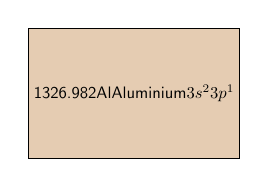
\begin{tikzpicture}[font=\sffamily, scale=0.6, transform shape]
   
  \tikzstyle{PostTranMetalFill} = [fill=brown!40]
  \tikzstyle{Element} = [draw=black, minimum width=2.75cm, minimum height=2.75cm, node distance=2.75cm]
  \tikzstyle{PostTranMetal} = [Element, PostTranMetalFill]
  \tikzstyle{PeriodLabel} = [font={\sffamily\LARGE}, node distance=2.0cm]
  \tikzstyle{CoreLabel} = [font={\sffamily\LARGE}, node distance=0.75cm]
  \tikzstyle{CoreLabelLaAc} = [font={\sffamily\LARGE}, node distance=2.0cm]
  \tikzstyle{CoreLegend} = [font={\sffamily\LARGE}, node distance=2.25cm]
  \tikzstyle{GroupLabel} = [font={\sffamily\LARGE}, minimum width=2.75cm, node distance=2.0cm]
  \tikzstyle{TitleLabel} = [font={\sffamily\Huge\bfseries}]

  \node[name=Al, PostTranMetal] {\NaturalElementTextFormat{13}{26.982}{Al}{Aluminium}{$3s^{2}3p^{1}$}};
  
\end{tikzpicture}
\end{center}

%\end{document}
 
\begin{description}
	\item[Symbole :] Al
	\item[Famille :] métaux de transitions
	\item[Numéro atomique \emph{Z} :] 13 protons
	\item[Nombre d'électrons :] 13 protons
	\item[Nombre de neutrons \emph{N} :] 14 neutrons pour l'isotope le plus abondant
	\item[Nombre de masse \emph{A} :] 27 nucléons
	\item[Masse molaire \emph{M} :] $M=\SI{26.981386}{\gram\per\mole}$ %appel de l'environnement de programmation des unités et des listes de nombres
	\item[Formule électronique/quantique :] $1s^{2}2s^{2}2p^{6}3s^{2}3p^{1}$ %appel de l'environnement de programmation des formules mathématiques
\end{description}

\pagebreak

\subsection{Configuration électronique}

\begin{figure}[h] %insertion d'une figure avec imposition de l'emplacement vertical (Here!) avec annotation et légende
	\begin{annotate}
		{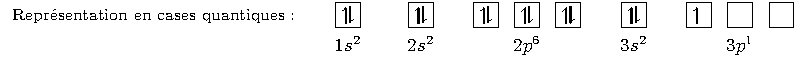
\includegraphics[scale=1]{tab_aluminium_configuration_electronique.pdf}}{0.1} %appel de la figure à annoter avec l'échelle des flèches et la grille de repères
		%\helpgrid[gray]  %grille d'aide pour le placement des objets (fonctionne aussi avec \DrawGrid{(-xmin,-ymin)}{(xmax,ymax)}

		\callout{-15,-10}{\cstep\label{pas:1}}{-11,-4} %flèche avec numéro référencé
		\callout{-6,-10}{\cstep\label{pas:2}}{-7.8,-2.6} %flèche avec numéro référencé
		\callout{8,-10}{\cstep\label{pas:3}}{13,2}
		\callout{3,-10}{\cstep\label{pas:4}}{3,-4}
		\callout{30,-10}{\cstep\label{pas:5}}{37,0.5}
		\draw [decorate,decoration={brace, raise=0.2cm}] (11.8,4.7) -- (30.1,4.7)
			node[above=0.2cm,pos=0.5] {\cstep\label{pas:6}};
		\draw [decorate,decoration={brace, raise=0.2cm}] (36.8,4.7) -- (66.2,4.7)
			node[above=0.2cm,pos=0.5] {\cstep\label{pas:7}};
	\end{annotate} 
\end{figure}

\begin{minipage}{\linewidth} %usage d'un environnement mini-page pour éviter les décalage au début de la première colonne quand l'élément n'est pas du texte simple
	\begin{multicols}{2} %répartition du texte dans l'environnement en deux colonnes
		\circref{pas:1}couche électronique $n=K$\\ %légende automatique
		\circref{pas:2}nombre d'électrons présents dans la sous-couche électronique $\ell=s$ de la couche électronique $n=K$\\
		\circref{pas:3}électron dans le sens de rotation du spin $m_{S}=-\frac{1}{2}$\\
		\circref{pas:4}sous-couche électronique $\ell=s$ de la couche électronique $n=L$\\
		\circref{pas:5}paire d'électrons de la sous-couche $\ell=s$ de la couche électronique électronique $n=M$ différenciés par le signe du nombre quantique du spin $S$
		\columnbreak\\ %passage à la deuxième colonne
		\circref{pas:6}cases quantiques désignant les nombres quantiques magnétiques du spin $M_S$ des électrons de la sous-couche $\ell=p$ de la couche électronique électronique $n=L$\\
		\circref{pas:7}dernière couche électronique $n=M$ (couche de valence)
	\end{multicols}
\end{minipage}

\subsection{Représentations graphiques}

\begin{center}
\begin{figure}[h] %insertion d'une figure avec imposition de l'emplacement vertical (Here!) avec annotation et légende
\startcstep %remet les compteurs des légendes en pastille à zéro
	\begin{minipage}{.69\linewidth}
		\begin{annotate}
			{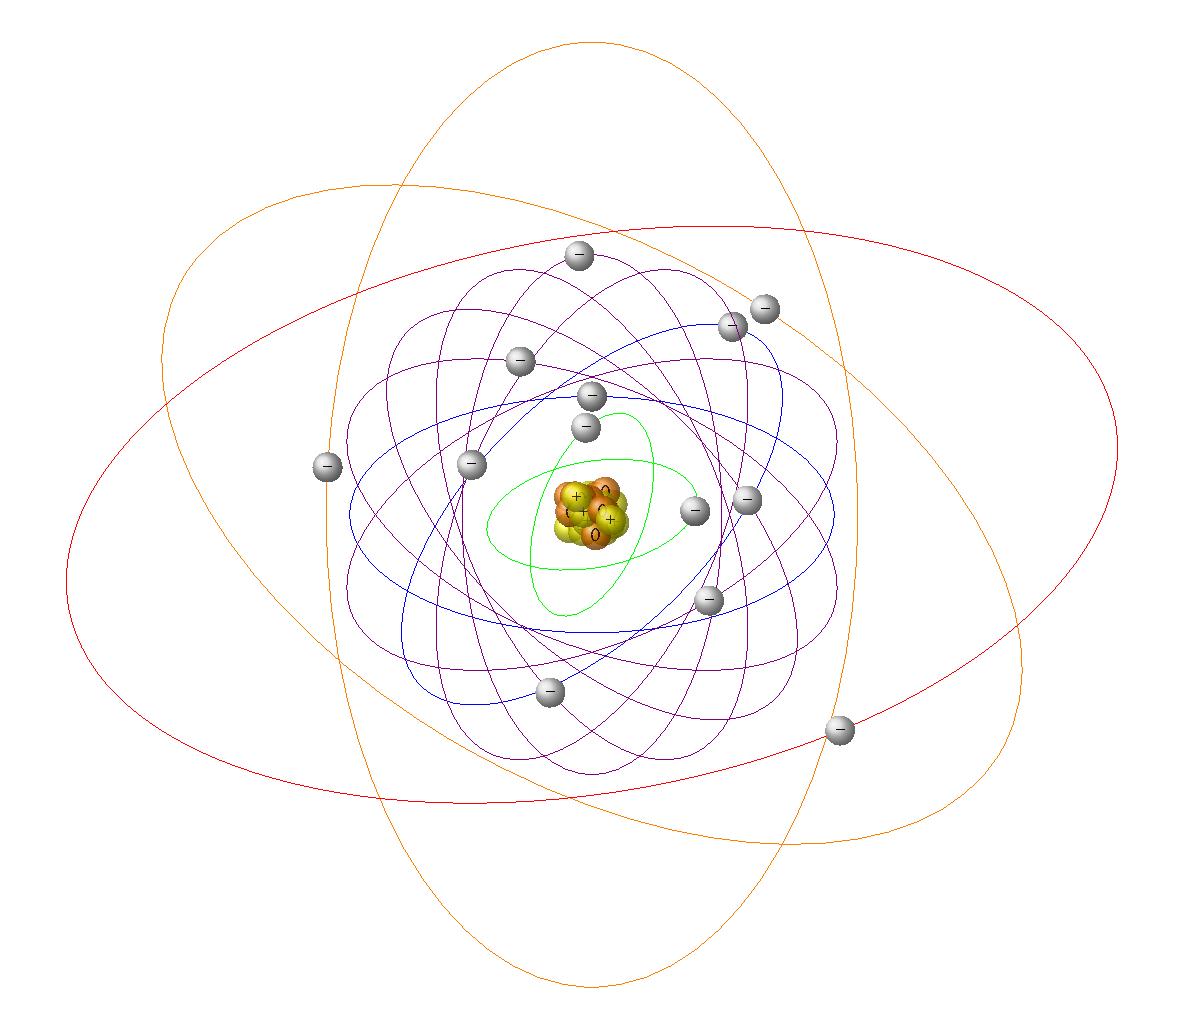
\includegraphics[scale=.6]{fig_aluminium_modelisation.pdf}}{0.5} %appel de la figure à annoter avec l'échelle des flèches et la grille de repères
			%\DrawGrid{(-12,-12)}{(12,12)} %grille d'aide pour le placement des objets

			\callout{7,8}{\cstep\label{pas:1}}{6,5.45}
			\callout{3,10}{\cstep\label{pas:2}}{1.9,9} %flèche avec numéro référencé
			\callout{7,-5}{\cstep\label{pas:3}}{5.3,-4.5}
			\callout{3,7}{\cstep\label{pas:4}}{3.5,4.5}
			\callout{7,-1.5}{\cstep\label{pas:5}}{5,-1.5}
			\callout{-7,-2.4}{\cstep\label{pas:6}}{-3.9,-2.4}
			\callout{-7,8}{\cstep\label{pas:7}}{-1.3,0.7}
			\callout{7,3}{\cstep\label{pas:8}}{0.6,0.6}
		\end{annotate} 
	\end{minipage}
\hfill
	\begin{minipage}{.28\linewidth}
\circref{pas:1}couche électronique M\\sous-couche p (bande de conduction)\\
\circref{pas:2}couche électronique M\\sous-couche s (valence) \\
\circref{pas:3}électron libre\\
\circref{pas:4}électron de valence\\
\circref{pas:5}couche électronique K\\sous-couche p\\
\circref{pas:6}couche électronique K\\sous-couche s\\
\circref{pas:7}couche électronique L\\sous-couche s\\
\circref{pas:8}noyau atomique
	\end{minipage}
	\caption{Modélisation détaillée (animation à la \superref{fig:aluminium_modelisation_animee})}
	\label{fig:aluminium_modelisation}
\end{figure}
\end{center}

\begin{center}
\begin{figure}[h] %insertion d'une figure avec imposition de l'emplacement vertical (Here!)
	\begin{subfigure}[b]{.46\linewidth} %appel de l'environnement pour la première de deux figures côte-à-côte
	\centering %figure centrée horizontalement
	\Lewis{0.2.4.,Al}
	\subcaption{Lewis}
	\label{fig:aluminium_lewis}
	\end{subfigure}
\hfill %impose l'écartement entre les deux figures
	\begin{subfigure}[b]{.46\linewidth} %appel de l'environnement pour la deuxième de deux figures côte-à-côte
		\begin{tikzpicture}
			\setbohr{distribution-method=quantum, insert-missing=true, } %représentation de Bohr
			\bohr{}{Al}
		\end{tikzpicture}
		\subcaption[b]{Rutherford-Bohr}
		\label{fig:aluminium_bohr}
	\end{subfigure}
	\caption{Représentation atomique de Lewis et de Bohr}
\end{figure}
\end{center}

\`A l'état fondamental, l'atome d'aluminium possède trois électrons de valence sur sa dernière couche électronique $3s^{\Circled{2}}\overset{\overset{+}{~}}{~}3p^{\Circled{1}}$. %symbole + au-dessus


%\end{document}


	%--------------------------------------
%chap_2_chimie_conduction_electrique
%--------------------------------------

\begin{comment}

\documentclass[a4paper, 11pt, twoside, fleqn]{memoir}

\usepackage{AOCDTF}

%--------------------------------------
%CANEVAS
%--------------------------------------

\newcommand\BoxColor{\ifcase\thechapshift blue!30\or brown!30\or pink!30\or cyan!30\or green!30\or teal!30\or purple!30\or red!30\or olive!30\or orange!30\or lime!30\or gray!\or magenta!30\else yellow!30\fi} %définition de la couleur des marqueurs de chapitre

\newcounter{chapshift} %compteur de chapitre du marqueur de chapitre
\addtocounter{chapshift}{-1}
	
\newif\ifFrame %instruction conditionnelle pour les couleurs des pages
\Frametrue

\pagestyle{plain}

% the main command; the mandatory argument sets the color of the vertical box
\newcommand\ChapFrame{%
\AddEverypageHook{%
\ifFrame
\ifthenelse{\isodd{\value{page}}}
  {\backgroundsetup{contents={%
  \begin{tikzpicture}[overlay,remember picture]
  \node[
  	rounded corners=3pt,
    fill=\BoxColor,
    inner sep=0pt,
    rectangle,
    text width=1.5cm,
    text height=5.5cm,
    align=center,
    anchor=north west
  ] 
  at ($ (current page.north west) + (-0cm,-2*\thechapshift cm) $) %nombre négatif = espacement des marqueurs entre les différents chapitres (à régler en fin de rédaction) (4.5cm vaut un espacement équivalement à la hauteur du marqueur, une page peut en contenir 6 avec cet espacement-la mais il est le plus équilibré)
    {\rotatebox{90}{\hspace*{.5cm}%
      \parbox[c][1.2cm][t]{5cm}{%
        \raggedright\textcolor{black}{\sffamily\textbf{\leftmark}}}}};
  \end{tikzpicture}}}
  }
  {\backgroundsetup{contents={%
  \begin{tikzpicture}[overlay,remember picture]
  \node[
  	rounded corners=3pt,
    fill=\BoxColor,
    inner sep=0pt,
    rectangle,
    text width=1.5cm,
    text height=5.5cm,
    align=center,
    anchor=north east
  ] 
  at ($ (current page.north east) + (-0cm,-2*\thechapshift cm) $) %nombre négatif = espacement des marqueurs entre les différents chapitres (à régler en fin de rédaction) (4.5cm vaut un espacement équivalement à la hauteur du marqueur, une page peut en contenir 6 avec cet espacement-la mais il est le plus équilibré)
    {\rotatebox{90}{\hspace*{.5cm}%
      \parbox[c][1.2cm][t]{5cm}{%
        \raggedright\textcolor{black}{\sffamily\textbf{\leftmark}}}}};
  \end{tikzpicture}}}%
  }
  \BgMaterial%
  \fi%
}%
  \stepcounter{chapshift}
}

\renewcommand\chaptermark[1]{\markboth{\thechapter.~#1}{}} %redéfinition du marqueur de chapitre pour ne contenir que le titre du chapitre

%utiliser les environnement \begin{comment} \end{comment} pour mettre en commentaire le préambule une fois la programmation appelée dans le fichier maître

%--------------------------------------
%corps du document
%--------------------------------------

\begin{document} %corps du document
	\openleft %début de chapitre à gauche
	\Frametrue %défini la booléenne Frame comme vrai -> marqueurs de chapitre

\end{comment}


\chapter{Chimie de la conduction électrique}
\ChapFrame %appel du marqueur de chapitre

\section{Dernière couche électronique}

\subsection{\'Electron-volt}

Les couches électroniques $K, L, M\ldots$ répartissent les électrons autour du noyau atomique :
\begin{itemize}
\item Plus un électron est proche du noyau atomique, plus l'énergie nécessaire pour arracher l'électron du champ électrique du noyau sera grande\,;
\item \'Energie quantifiée en \emph{électron-volt} \si{\electronvolt}.
\end{itemize}
Un \emph{électron-volt} est la mesure physique de l'énergie cinétique d'un électron accéléré sous l'action d'une \emph{différence de potentiel} d'$\SI{1}{\volt}$. Il est égal à : 

\begin{formule}{Valeur expérimentale de l'\electronvolt}{valeur_experimentale_electronvolt}
	\begin{align} 
		U &= \frac{W}{Q} \\
		\electronvolt &= \sqrt{\frac{2h\alpha}{\mu\clight}}\frac{W}{Q} \\
		&=\SI{1,602176634e-19}{\joule} \nonumber
	\end{align}

\begin{numvariables}
U						& différence de potentiel					& volt						& \volt								& \volt  				& \si{\kilogram\square\meter\per\cubic\second\per\ampere} \\
W						& énergie											& joule						& \joule								& \joule				& \si{kg.m^{2}/s^{2}} \\
Q						& charge électrique							& coulomb					& \coulomb						& \coulomb		& \si{\ampere\second} \\
\electronvolt 		& électron-volt 									& joule 					& \si\joule 							& \electronvolt	& \SI{1,602176634e-19}{\joule} \\
h 						& constante de Planck 						& joule seconde 		& \si{\joule\second	}			& h					& \SI{6,62607015e-34}{\joule\second} \\
\alpha				& constante de structure fine 				& sans dimension 		&										& \alpha			& \num{7,2973525564e-3} \\
\mu					& perméabilité magnétique du vide	& henry par mètre		& \si{\henry\per\meter}		& \mu				& \SI{4\pi e-7}{\henry\per\meter} \\
\clight				& vitesse de la lumière dans le vide	& mètre par seconde & \si{\meter\per\second}	& \clight			& \SI{2,99792458e8}{\meter\per\second}	
\end{numvariables}
\end{formule}



%\end{document}



	%--------------------------------------
	%style des annexes
	%--------------------------------------

	\Framefalse %défini la booléenne Frame comme false -> pas de marqueurs de chapitre
	\appendix %appel des annexes
	\appendixpage

	%--------------------------------------
	%inclusion des chapitres
	%--------------------------------------

	%utiliser les environnement \begin{comment} \end{comment} pour mettre en commentaire le préambule une fois la programmation appelée dans le document maître (!ne pas oublier de mettre en commentaire \end{document}!)

%--------------------------------------
%chap_A_addendeum_chimie_atomique
%--------------------------------------

\begin{comment}

\documentclass[a4paper, 11pt, twoside]{memoir}

\usepackage{AOCDTF}

%--------------------------------------
%CANEVAS
%--------------------------------------

\newcommand\BoxColor{\ifcase\thechapshift blue!30\or brown!30\or pink!30\or cyan!30\or green!30\or teal!30\or purple!30\or red!30\or olive!30\or orange!30\or lime!30\or gray!\or magenta!30\else yellow!30\fi} %définition de la couleur des marqueurs de chapitre

\newcounter{chapshift} %compteur de chapitre du marqueur de chapitre
\addtocounter{chapshift}{-1}
	
\newif\ifFrame %instruction conditionnelle pour les couleurs des pages
\Frametrue

\pagestyle{plain}

% the main command; the mandatory argument sets the color of the vertical box
\newcommand\ChapFrame{%
\AddEverypageHook{%
\ifFrame
\ifthenelse{\isodd{\value{page}}}
  {\backgroundsetup{contents={%
  \begin{tikzpicture}[overlay,remember picture]
  \node[
  	rounded corners=3pt,
    fill=\BoxColor,
    inner sep=0pt,
    rectangle,
    text width=1.5cm,
    text height=5.5cm,
    align=center,
    anchor=north west
  ] 
  at ($ (current page.north west) + (-0cm,-2*\thechapshift cm) $) %nombre négatif = espacement des marqueurs entre les différents chapitres (à régler en fin de rédaction) (4.5cm vaut un espacement équivalement à la hauteur du marqueur, une page peut en contenir 6 avec cet espacement-la mais il est le plus équilibré)
    {\rotatebox{90}{\hspace*{.5cm}%
      \parbox[c][1.2cm][t]{5cm}{%
        \raggedright\textcolor{black}{\sffamily\textbf{\leftmark}}}}};
  \end{tikzpicture}}}
  }
  {\backgroundsetup{contents={%
  \begin{tikzpicture}[overlay,remember picture]
  \node[
  	rounded corners=3pt,
    fill=\BoxColor,
    inner sep=0pt,
    rectangle,
    text width=1.5cm,
    text height=5.5cm,
    align=center,
    anchor=north east
  ] 
  at ($ (current page.north east) + (-0cm,-2*\thechapshift cm) $) %nombre négatif = espacement des marqueurs entre les différents chapitres (à régler en fin de rédaction) (4.5cm vaut un espacement équivalement à la hauteur du marqueur, une page peut en contenir 6 avec cet espacement-la mais il est le plus équilibré)
    {\rotatebox{90}{\hspace*{.5cm}%
      \parbox[c][1.2cm][t]{5cm}{%
        \raggedright\textcolor{black}{\sffamily\textbf{\leftmark}}}}};
  \end{tikzpicture}}}%
  }
  \BgMaterial%
  \fi%
}%
  \stepcounter{chapshift}
}

\renewcommand\chaptermark[1]{\markboth{\thechapter.~#1}{}} %redéfinition du marqueur de chapitre pour ne contenir que le titre du chapitre %à personnaliser selon le nombre de chapitre dans le cours

%--------------------------------------
%corps du document
%--------------------------------------

\begin{document} %corps du document
	\openleft %début de chapitre à gauche

\end{comment}

\chapter{Addendum de chimie atomique}
\label{ann:addendum_chimie_atomique}

Cet annexe regroupe tous les tableaux et figures mentionnés dans le \superref{chap:chimie_atomique} qui contiennent un nombre importants de données. Il n'est pas nécessaire de les retenir par c\oe{}ur mais ces informations constituent un support appréciable pour toute précision concernant ce chapitre.

%--------------------------------------
%PRE-REQUIS
%--------------------------------------

%utiliser les environnement \begin{comment} \end{comment} pour mettre en commentaire le préambule une fois la programmation appelée dans le document maître (!ne pas oublier de mettre en commentaire \end{document}!)

\documentclass[a4paper, 11pt, twoside, fleqn]{memoir}

\usepackage{AOCDTF}

%--------------------------------------
%CANEVAS
%--------------------------------------

\newcommand\BoxColor{\ifcase\thechapshift blue!30\or brown!30\or pink!30\or cyan!30\or green!30\or teal!30\or purple!30\or red!30\or olive!30\or orange!30\or lime!30\or gray!\or magenta!30\else yellow!30\fi} %définition de la couleur des marqueurs de chapitre

\newcounter{chapshift} %compteur de chapitre du marqueur de chapitre
\addtocounter{chapshift}{-1}
	
\newif\ifFrame %instruction conditionnelle pour les couleurs des pages
\Frametrue

\pagestyle{plain}

% the main command; the mandatory argument sets the color of the vertical box
\newcommand\ChapFrame{%
\AddEverypageHook{%
\ifFrame
\ifthenelse{\isodd{\value{page}}}
  {\backgroundsetup{contents={%
  \begin{tikzpicture}[overlay,remember picture]
  \node[
  	rounded corners=3pt,
    fill=\BoxColor,
    inner sep=0pt,
    rectangle,
    text width=1.5cm,
    text height=5.5cm,
    align=center,
    anchor=north west
  ] 
  at ($ (current page.north west) + (-0cm,-2*\thechapshift cm) $) %nombre négatif = espacement des marqueurs entre les différents chapitres (à régler en fin de rédaction) (4.5cm vaut un espacement équivalement à la hauteur du marqueur, une page peut en contenir 6 avec cet espacement-la mais il est le plus équilibré)
    {\rotatebox{90}{\hspace*{.5cm}%
      \parbox[c][1.2cm][t]{5cm}{%
        \raggedright\textcolor{black}{\sffamily\textbf{\leftmark}}}}};
  \end{tikzpicture}}}
  }
  {\backgroundsetup{contents={%
  \begin{tikzpicture}[overlay,remember picture]
  \node[
  	rounded corners=3pt,
    fill=\BoxColor,
    inner sep=0pt,
    rectangle,
    text width=1.5cm,
    text height=5.5cm,
    align=center,
    anchor=north east
  ] 
  at ($ (current page.north east) + (-0cm,-2*\thechapshift cm) $) %nombre négatif = espacement des marqueurs entre les différents chapitres (à régler en fin de rédaction) (4.5cm vaut un espacement équivalement à la hauteur du marqueur, une page peut en contenir 6 avec cet espacement-la mais il est le plus équilibré)
    {\rotatebox{90}{\hspace*{.5cm}%
      \parbox[c][1.2cm][t]{5cm}{%
        \raggedright\textcolor{black}{\sffamily\textbf{\leftmark}}}}};
  \end{tikzpicture}}}%
  }
  \BgMaterial%
  \fi%
}%
  \stepcounter{chapshift}
}

\renewcommand\chaptermark[1]{\markboth{\thechapter.~#1}{}} %redéfinition du marqueur de chapitre pour ne contenir que le titre du chapitre %à personnaliser selon le nombre de chapitre dans le cours

%--------------------------------------
%corps du document
%--------------------------------------

\begin{document} %corps du document
	\openleft %début de chapitre à gauche


\begin{table}[!h]
\begin{center}
\caption{Distribution des électrons dans les orbitales atomiques par sous-couche électronique\label{tab:exception_hund}\supercite{Wiki:TPE}}

\begin{threeparttable} %note dans tableau
\begin{tabularx}{\textwidth}{r c l X l @{\hspace{2cm}}X} \\ %tableau de plusieurs à 5 colonnes
\toprule %filet de haut de tableau
\multicolumn{3}{c}{\thead{\'Elément chimique}} & \thead[l]{Famille} & \multicolumn{2}{l}{\thead[l]{Configuration électronique}} \\
\midrule
$24$ 	& Cr 		& Chrome 			& Métal de transition 		& [Ar] 		& $\mathbf{4s^1 3d^5}$ \\
$28$ 	& Ni		& Nickel 			& Métal de transition 		& [Ar] 		& $\mathbf{4s^1 3d^9}$ \tnote{(*)} \\
$29$ 	& Cu		& Cuivre 			& Métal de transition 		& [Ar] 		& $\mathbf{4s^1 3d^{10}}$ \\
$41$ 	& Nb 	&Niobium 			& Métal de transition 		& [Kr] 		& $\mathbf{5s^1 4d^4}$ \\
$42$ 	& Mo 	& Molybdène 	& Métal de transition 		& [Kr] 		& $\mathbf{5s^1 4d^5}$ \\
$44$ 	&Ru 		& Ruthénium 	& Métal de transition 		& [Kr] 		& $\mathbf{5s^1 4d^7}$ \\
$45$		& Rh 	& Rhodium 		& Métal de transition	 	& [Kr] 		& $\mathbf{5s^1 4d^8}$ \\
$46$ 	& Pd 		& Palladium 		& Métal de transition 		& [Kr] 		& $\mathbf{4d^{10}}$ \\
$47$ 	& Ag 	& Argent 			& Métal de transition 		& [Kr] 		& $\mathbf{5s^1 4d^{10}}$ \\
$57$	 	& La 		& Lanthane 		& Lanthanide 				& [Xe] 		& $6s^2 \mathbf{5d^1}$ \\
$58$ 	& Ce 		& Cérium 			& Lanthanide 				& [Xe] 		& $6s^2 \mathbf{4f^1 5d^1}$ \\
$64$	 	& Gd 	& Gadolinium 	& Lanthanide 				& [Xe] 		& $6s^2 \mathbf{4f^7 5d^1}$ \\
$78$ 	& Pt 		& Platine 			& Métal de transition 		& [Xe] 		& $\mathbf{6s^1} 4f^14 \mathbf{5d^9}$ \\
$79$ 	& Au 	& Or 					& Métal de transition 		& [Xe] 		& $\mathbf{6s^1} 4f^{14} \mathbf{5d^{10}}$ \\
$89$  	& Ac 		& Actinium 		& Actinide 					& [Rn] 		& $7s^2 \mathbf{6d^1}$ \\
$90$ 	& 	Th 	& Thorium 		& Actinide 					& [Rn] 		& $7s^2 \mathbf{6d^2} $ \\
$91$ 	& Pa 		& Protactinium	& Actinide 					& [Rn] 		& $7s^2 \mathbf{5f^2 6d^1}$ \\
$92$		& U 		& Uranium 		& Actinide 					& [Rn] 		& $7s^2 \mathbf{5f^3 6d^1}$ \\
$96$ 	& Cm 	& Curium 			& Actinide 					& [Rn] 		& $7s^2 \mathbf{5f^7 6d^1}$ \\
$103$	& Lr 		& Lawrencium 	& Actinide 					& [Rn] 		& $7s^2 \mathbf{5f^{14} 7p^1}$ \\

\bottomrule

\end{tabularx}
\begin{tablenotes}
    \item[(*)] Le nickel présente deux configurations électroniques :
    \begin{compactitemize}
    		\item Une configuration régulière [Ar] $4s^2 3d^8$ présentant le niveau d'énergie le plus bas expérimentalement\,;
    		\item Une configuration irrégulière [Ar] $4s^1 3d^9$ présentant le niveau d'énergie moyen le plus bas. C'est cette configuration qui sera utilisée dans les calculs. 
	\end{compactitemize}
\end{tablenotes}
\end{threeparttable}
\end{center}
\end{table}

\end{document}

\begin{landscape}
	\begin{figure}
	\caption{Tableau périodique des éléments chimiques}
	\label{tab:tableau_periodique}
		\begin{center}
			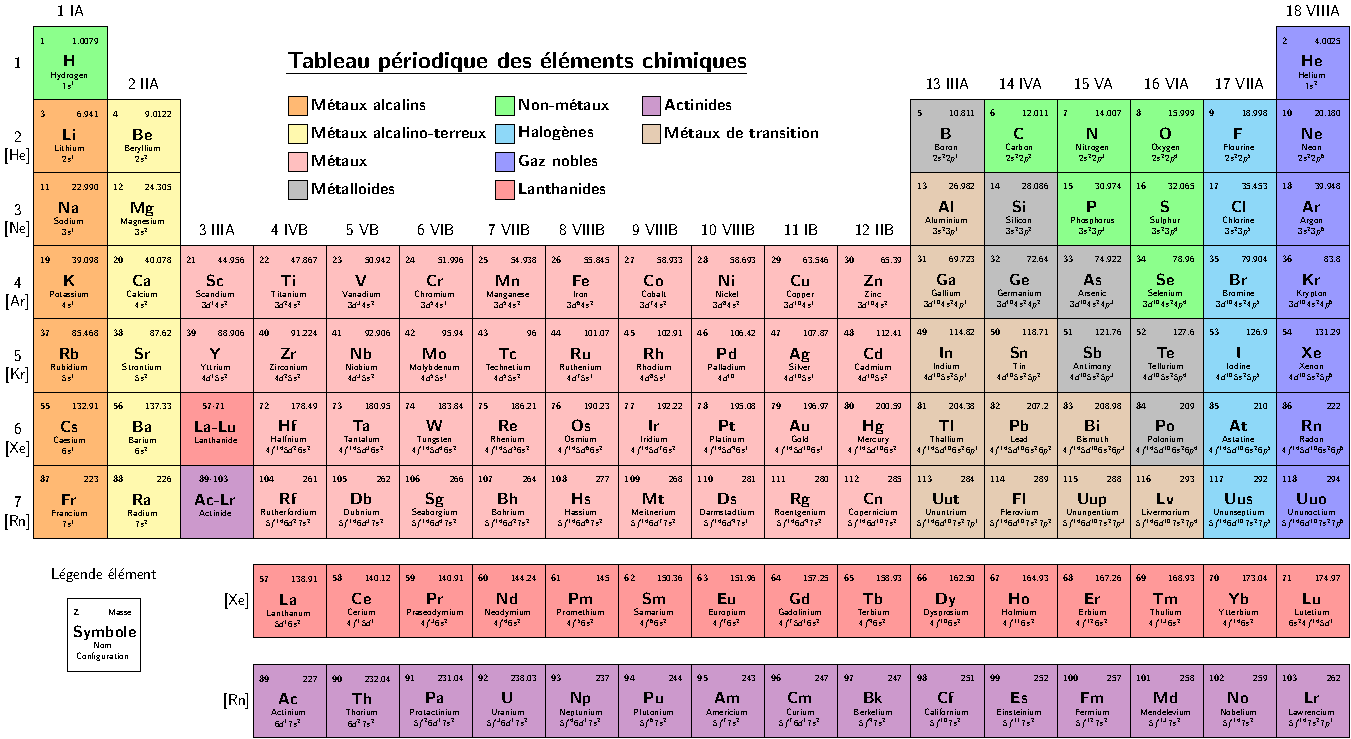
\includegraphics[scale=1.15]{tab_tableau_periodique.pdf} 
		\end{center}
	\end{figure}
\end{landscape}

%utiliser les environnement \begin{comment} \end{comment} pour mettre en commentaire le préambule une fois la programmation appelée dans le document maître (!ne pas oublier de mettre en commentaire \end{document}!)

\begin{comment}

\documentclass[a4paper, 11pt, twoside, fleqn]{memoir}

\usepackage{AOCDTF}

%--------------------------------------
%CANEVAS
%--------------------------------------

\newcommand\BoxColor{\ifcase\thechapshift blue!30\or brown!30\or pink!30\or cyan!30\or green!30\or teal!30\or purple!30\or red!30\or olive!30\or orange!30\or lime!30\or gray!\or magenta!30\else yellow!30\fi} %définition de la couleur des marqueurs de chapitre

\newcounter{chapshift} %compteur de chapitre du marqueur de chapitre
\addtocounter{chapshift}{-1}
	
\newif\ifFrame %instruction conditionnelle pour les couleurs des pages
\Frametrue

\pagestyle{plain}

% the main command; the mandatory argument sets the color of the vertical box
\newcommand\ChapFrame{%
\AddEverypageHook{%
\ifFrame
\ifthenelse{\isodd{\value{page}}}
  {\backgroundsetup{contents={%
  \begin{tikzpicture}[overlay,remember picture]
  \node[
  	rounded corners=3pt,
    fill=\BoxColor,
    inner sep=0pt,
    rectangle,
    text width=1.5cm,
    text height=5.5cm,
    align=center,
    anchor=north west
  ] 
  at ($ (current page.north west) + (-0cm,-2*\thechapshift cm) $) %nombre négatif = espacement des marqueurs entre les différents chapitres (à régler en fin de rédaction) (4.5cm vaut un espacement équivalement à la hauteur du marqueur, une page peut en contenir 6 avec cet espacement-la mais il est le plus équilibré)
    {\rotatebox{90}{\hspace*{.5cm}%
      \parbox[c][1.2cm][t]{5cm}{%
        \raggedright\textcolor{black}{\sffamily\textbf{\leftmark}}}}};
  \end{tikzpicture}}}
  }
  {\backgroundsetup{contents={%
  \begin{tikzpicture}[overlay,remember picture]
  \node[
  	rounded corners=3pt,
    fill=\BoxColor,
    inner sep=0pt,
    rectangle,
    text width=1.5cm,
    text height=5.5cm,
    align=center,
    anchor=north east
  ] 
  at ($ (current page.north east) + (-0cm,-2*\thechapshift cm) $) %nombre négatif = espacement des marqueurs entre les différents chapitres (à régler en fin de rédaction) (4.5cm vaut un espacement équivalement à la hauteur du marqueur, une page peut en contenir 6 avec cet espacement-la mais il est le plus équilibré)
    {\rotatebox{90}{\hspace*{.5cm}%
      \parbox[c][1.2cm][t]{5cm}{%
        \raggedright\textcolor{black}{\sffamily\textbf{\leftmark}}}}};
  \end{tikzpicture}}}%
  }
  \BgMaterial%
  \fi%
}%
  \stepcounter{chapshift}
}

\renewcommand\chaptermark[1]{\markboth{\thechapter.~#1}{}} %redéfinition du marqueur de chapitre pour ne contenir que le titre du chapitre %à personnaliser selon le nombre de chapitre dans le cours

%--------------------------------------
%corps du document
%--------------------------------------

\begin{document} %corps du document
	\openleft %début de chapitre à gauche

\end{comment}


\begin{landscape}
\begin{xltabular}{\linewidth}{C C C c c c c c c c}
\caption{Orbitales réelles d'un atome hydrogénoïde par triplet de nombres quantiques ($n, \ell, m_{\ell}$)\label{tab:geometrie_orbitale}\supercite{Wiki:OA}} 
\\
\toprule

\multicolumn{2}{c}{\thead{Nombre quantique}} & \multirow[c]{2}{*}{\thead{Sous-couche}} & \multicolumn{7}{c}{\thead{Module $\lvert M_\ell \rvert$ du nombre quantique magnétique}} \\

\cmidrule(lr){1-2} \cmidrule(lr){4-10} %filet de milieu de tableau centré sur les colonnes mentionnées

\thead{Principal} & \thead{Azimutal} & & \thead{$0$} & \multicolumn{2}{c}{\thead{$1$}} & \multicolumn{2}{c}{\thead{$2$}} & \multicolumn{2}{c}{\thead{$3$}} \\

\midrule %filet de milieu de tableau

\endfirsthead %en-tête de la première page du tableau  

\toprule

\multicolumn{2}{c}{\thead{Nombre quantique}} & \multirow[c]{2}{*}{\thead{Sous-couche}} & \multicolumn{7}{c}{\thead{Module $\lvert M_\ell \rvert$ du nombre quantique magnétique}} \\

\cmidrule(lr){1-2} \cmidrule(lr){4-10} %filet de milieu de tableau centré sur les colonnes mentionnées

\thead{Principal} & \thead{Azimutal} & & \thead{$0$} & \multicolumn{2}{c}{\thead{$1$}} & \multicolumn{2}{c}{\thead{$2$}} & \multicolumn{2}{c}{\thead{$3$}} \\

\midrule %filet de milieu de tableau

\endhead %en-tête de la première page du tableau
	\addlinespace
	\midrule %filet de milieu de tableau
	\multicolumn{10}{r}{\small\textit{Page suivante}}
\endfoot %pied de page de toutes les pages du tableau
\endlastfoot %pied de page de la dernièredu tableau

\multirow[t]{2}{*}{$n=1$} & \multirow[t]{2}{*}{$\ell=0$} & \multirow[t]{2}{*}{$1s$} & 
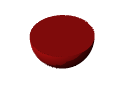
\includegraphics[width=1.6cm]{tableau_geometrie_orbitale_modelisation/S1M0.png} 

& & & & & & \\

& & & \makecell[c]{$1s$} & & & & & &  \\ %centrer la cellule individuellement horizontalement 

\midrule %filet de milieu de tableau

\multirow[t]{4}{*}{$n=2$} & \multirow[t]{2}{*}{$\ell=0$} & \multirow[t]{2}{*}{$2s$} & 
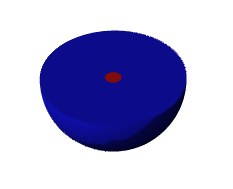
\includegraphics[width=1.6cm]{tableau_geometrie_orbitale_modelisation/S2M0.png} 
& & & & & & \\

& & & \makecell[c]{$2s$} & & & & & &  \\ %centrer la cellule individuellement 

\addlinespace

& \multirow[t]{2}{*}{$\ell=1$} & \multirow[t]{2}{*}{$2p$} & 
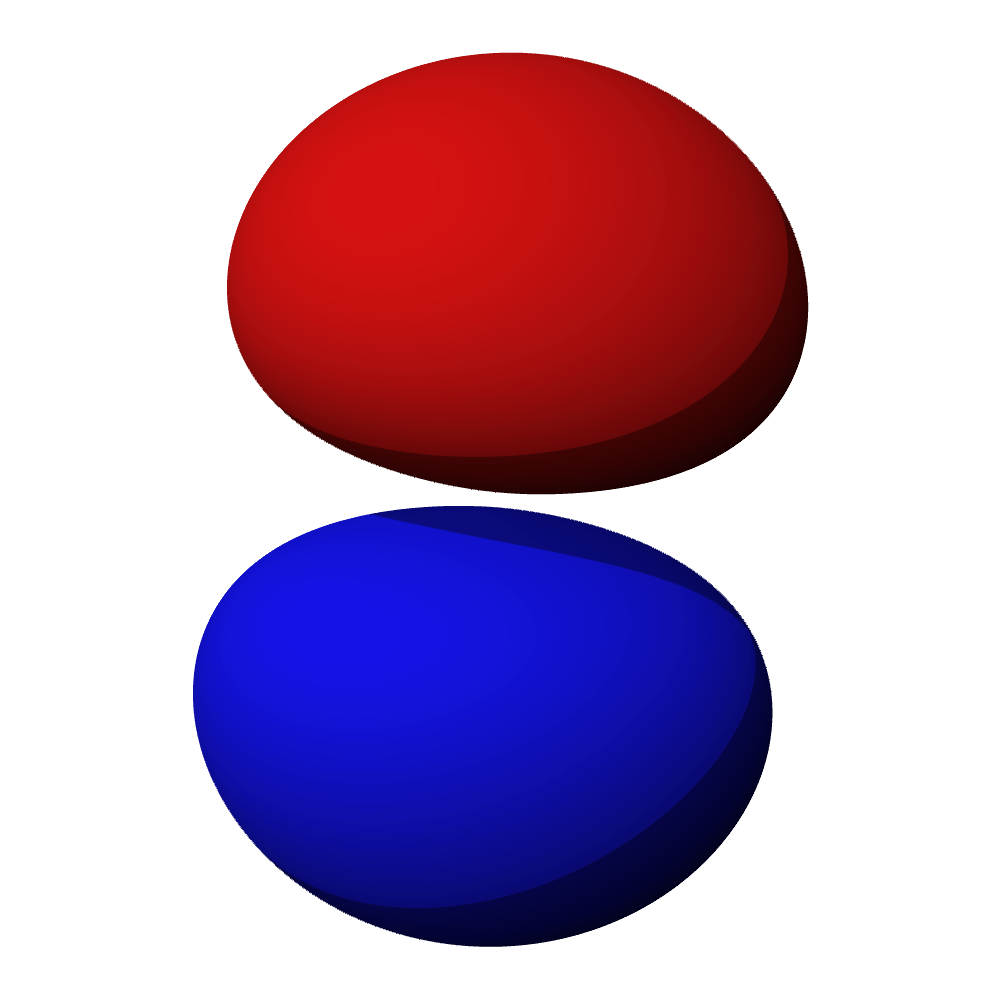
\includegraphics[width=1.6cm]{tableau_geometrie_orbitale_modelisation/Pz_orbital.png} 
&
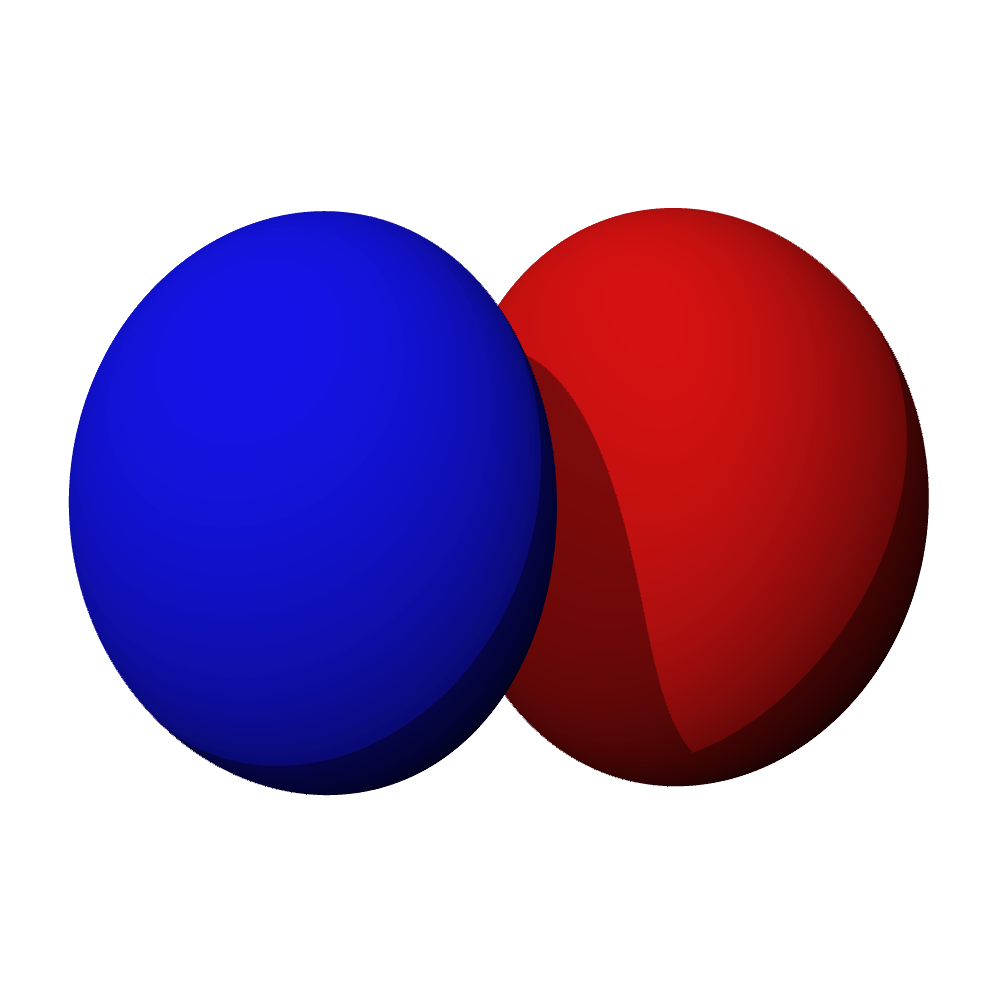
\includegraphics[width=1.6cm]{tableau_geometrie_orbitale_modelisation/Px_orbital.png}  
&
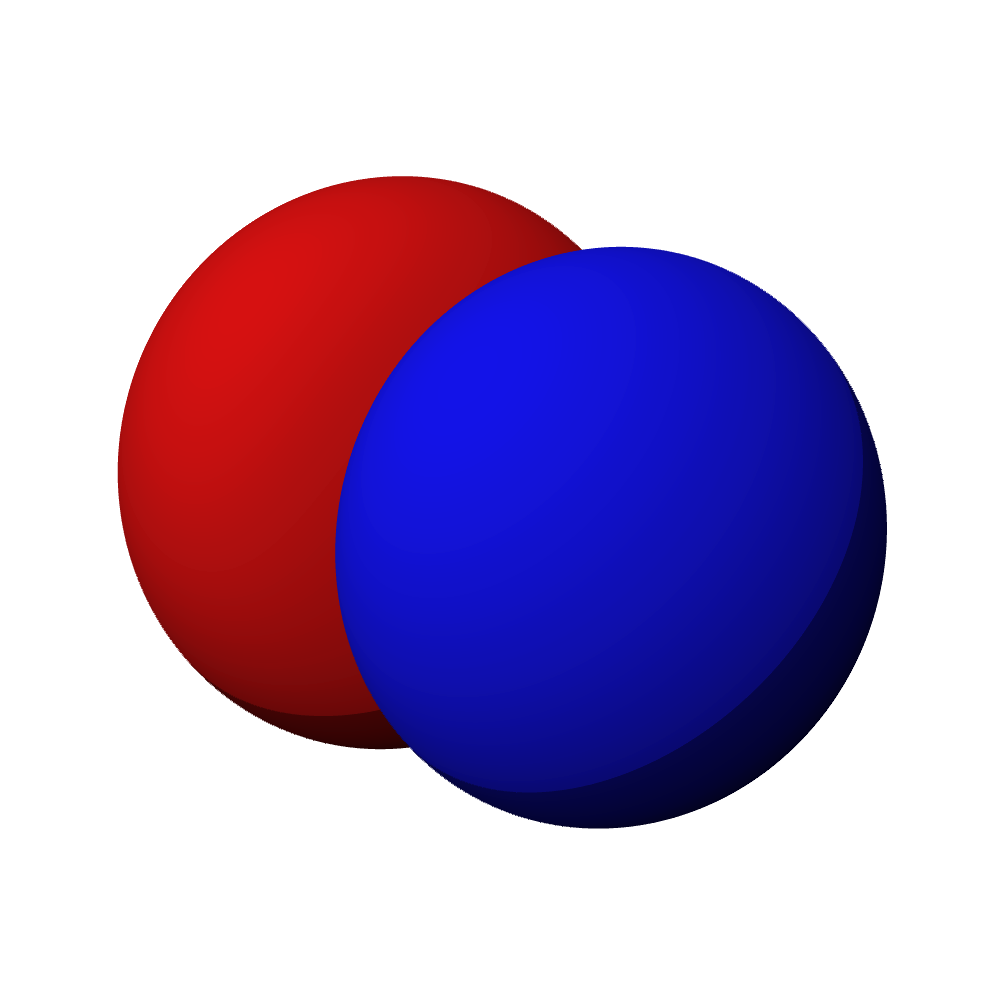
\includegraphics[width=1.6cm]{tableau_geometrie_orbitale_modelisation/Py_orbital.png} 
& & & & \\

& & & \makecell[c]{$2p_z$} & \makecell[c]{$2p_x$} & \makecell[c]{$2p_y$} & & & &  \\ %centrer la cellule individuellement 

\midrule %filet de milieu de tableau

\multirow[t]{6}{*}{$n=3$} & \multirow[t]{2}{*}{$\ell=0$} & \multirow[t]{2}{*}{$3s$} & 
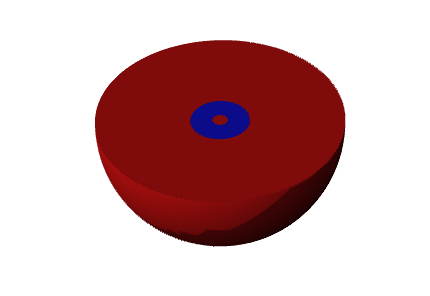
\includegraphics[width=1.6cm]{tableau_geometrie_orbitale_modelisation/S3M0.png} 
& & & & & & \\

& & & \makecell[c]{$3s$} & & & & & &  \\ %centrer la cellule individuellement 

\addlinespace

& \multirow[t]{2}{*}{$\ell=1$} & \multirow[t]{2}{*}{$3p$} & 
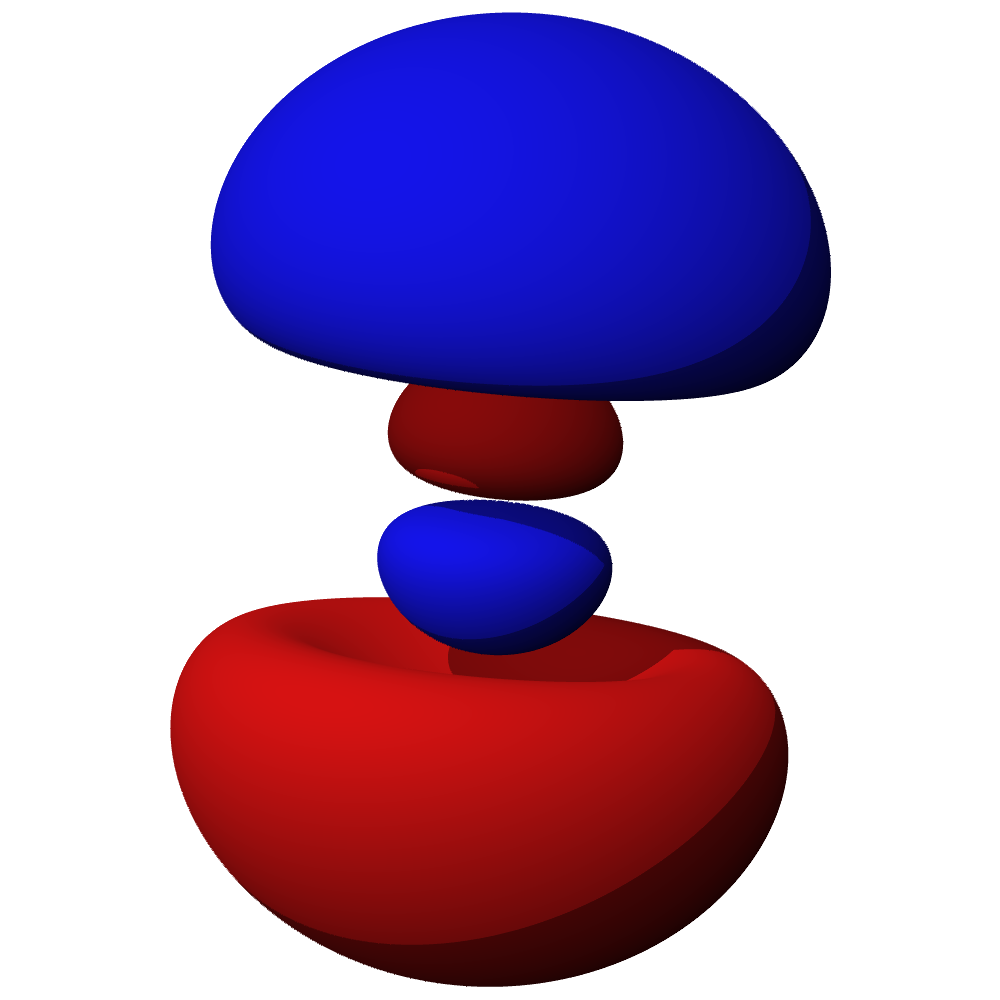
\includegraphics[width=1.6cm]{tableau_geometrie_orbitale_modelisation/P3z.png} 
&
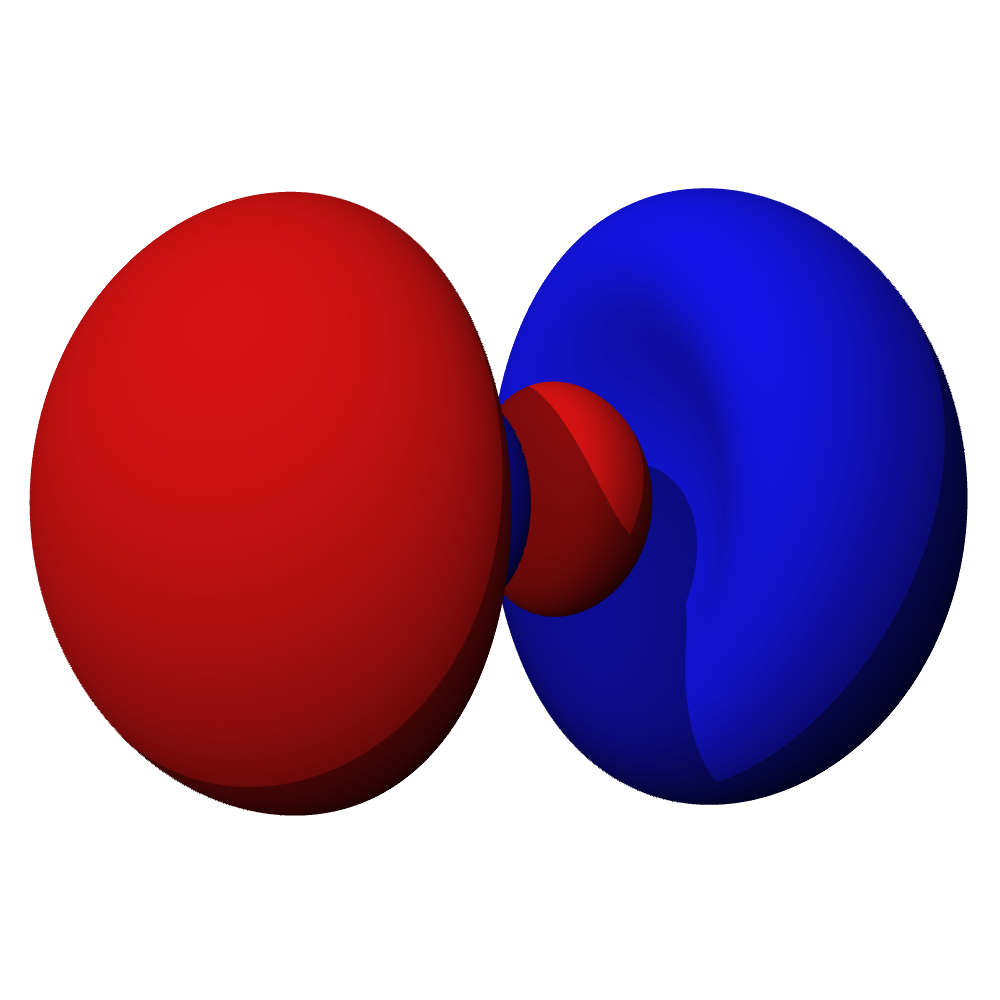
\includegraphics[width=1.6cm]{tableau_geometrie_orbitale_modelisation/P3x.png}  
&
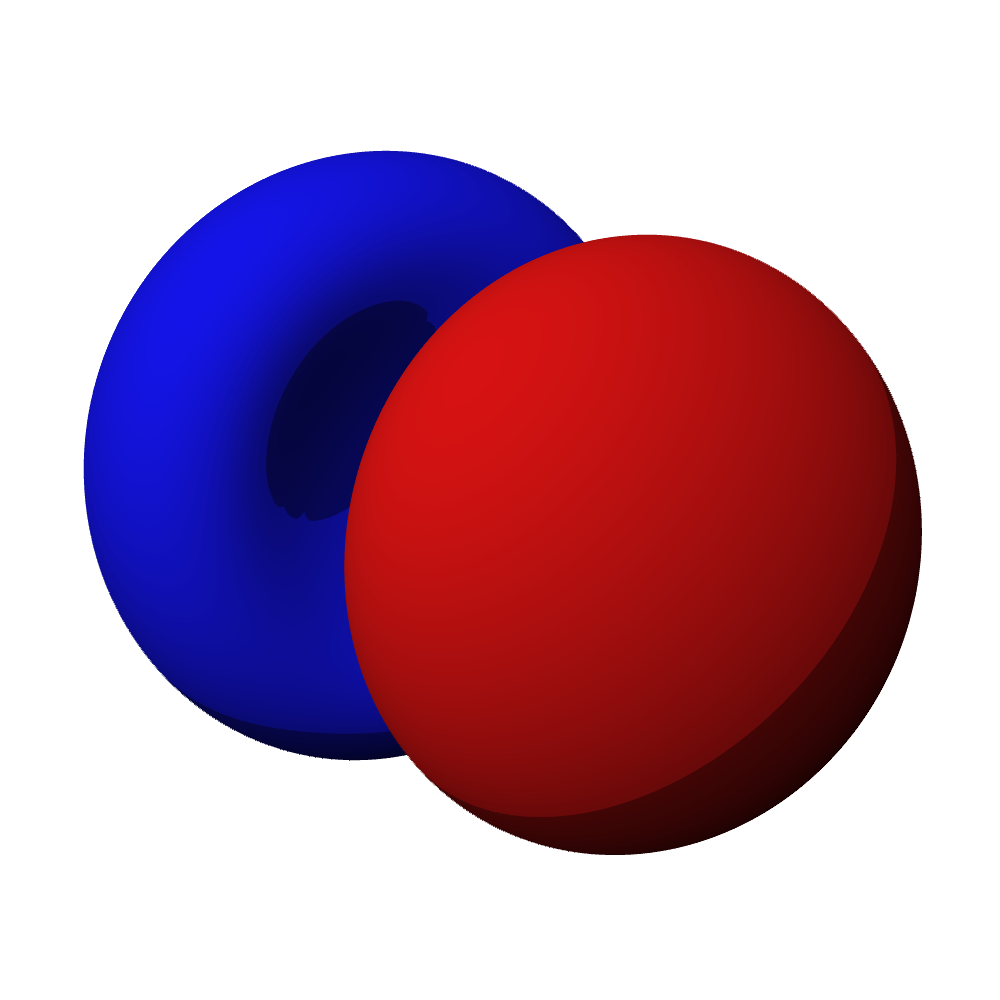
\includegraphics[width=1.6cm]{tableau_geometrie_orbitale_modelisation/P3y.png} 
& & & & \\

& & & \makecell[c]{$3p_z$} & \makecell[c]{$3p_x$} & \makecell[c]{$3p_y$} & & & &  \\ %centrer la cellule individuellement 

\addlinespace

 & \multirow[t]{2}{*}{$\ell=2$} & \multirow[t]{2}{*}{$3d$} & 
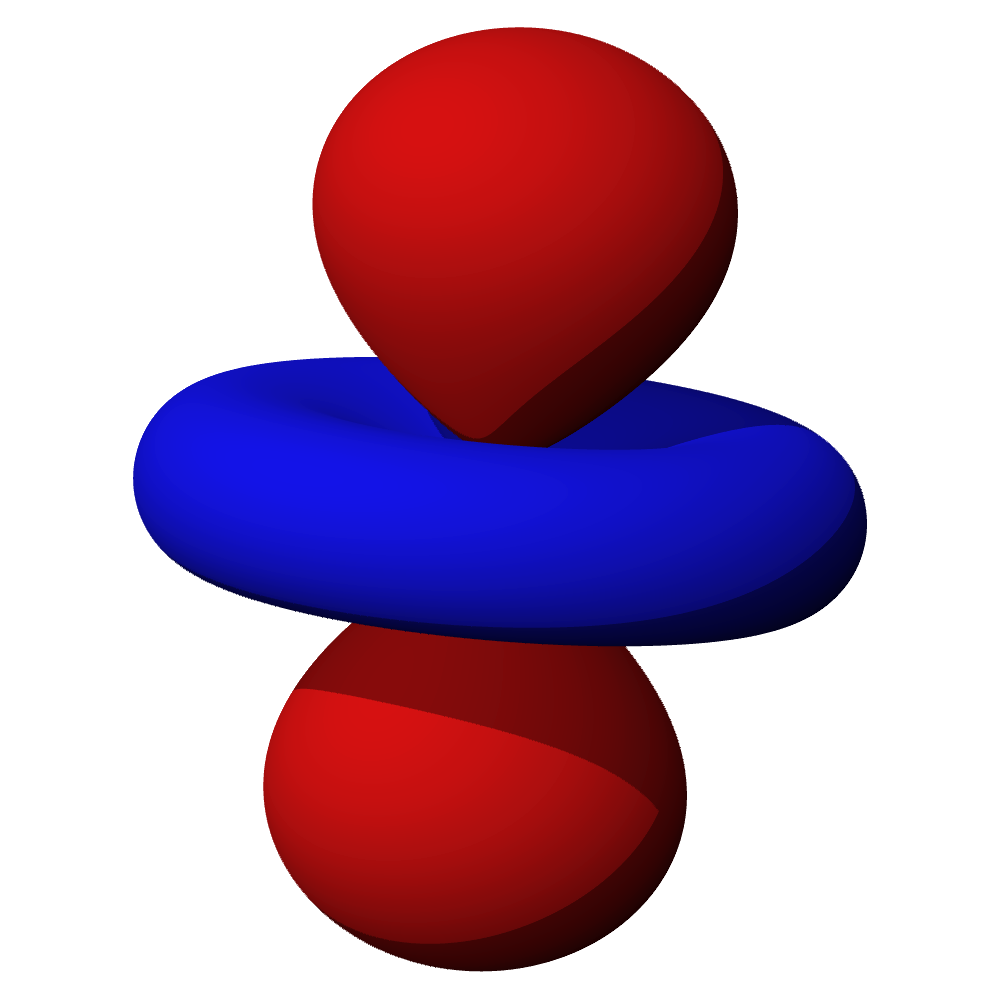
\includegraphics[width=1.6cm]{tableau_geometrie_orbitale_modelisation/Dz2_orbital.png} 
&
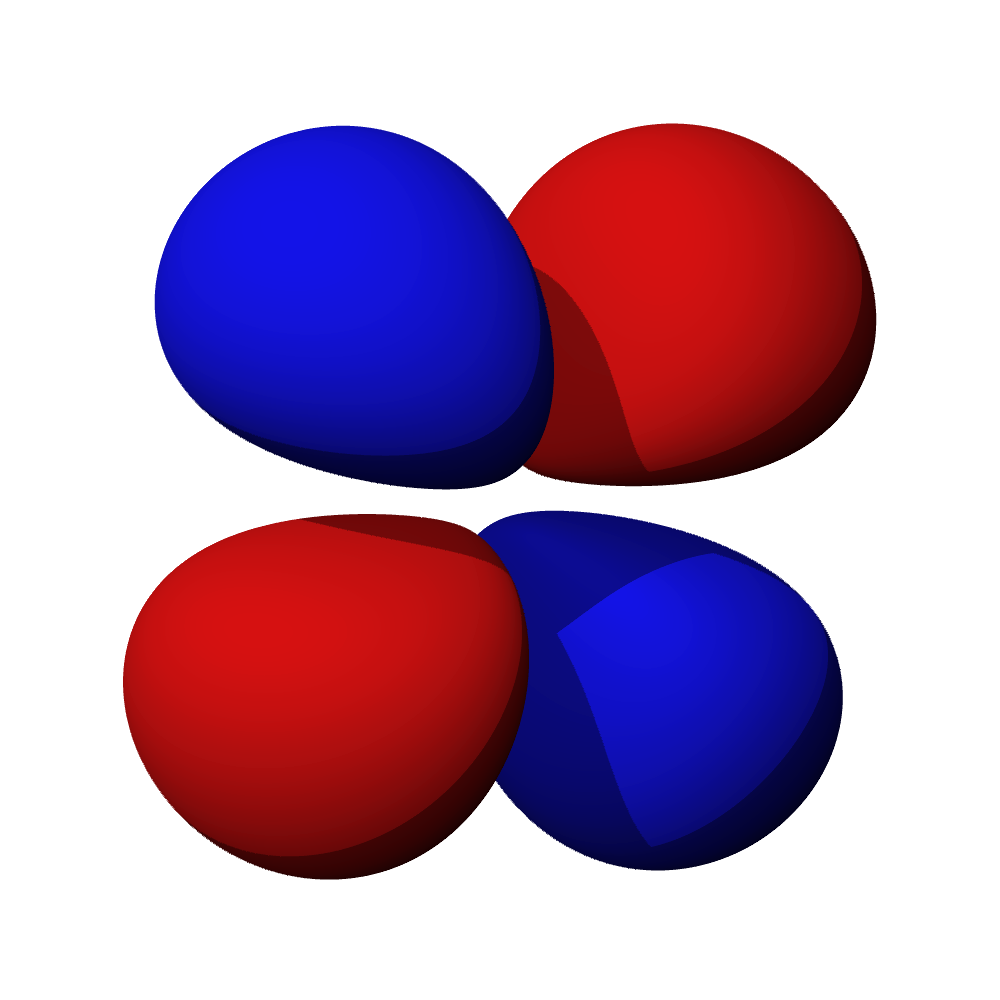
\includegraphics[width=1.6cm]{tableau_geometrie_orbitale_modelisation/Dxz_orbital.png}  
&
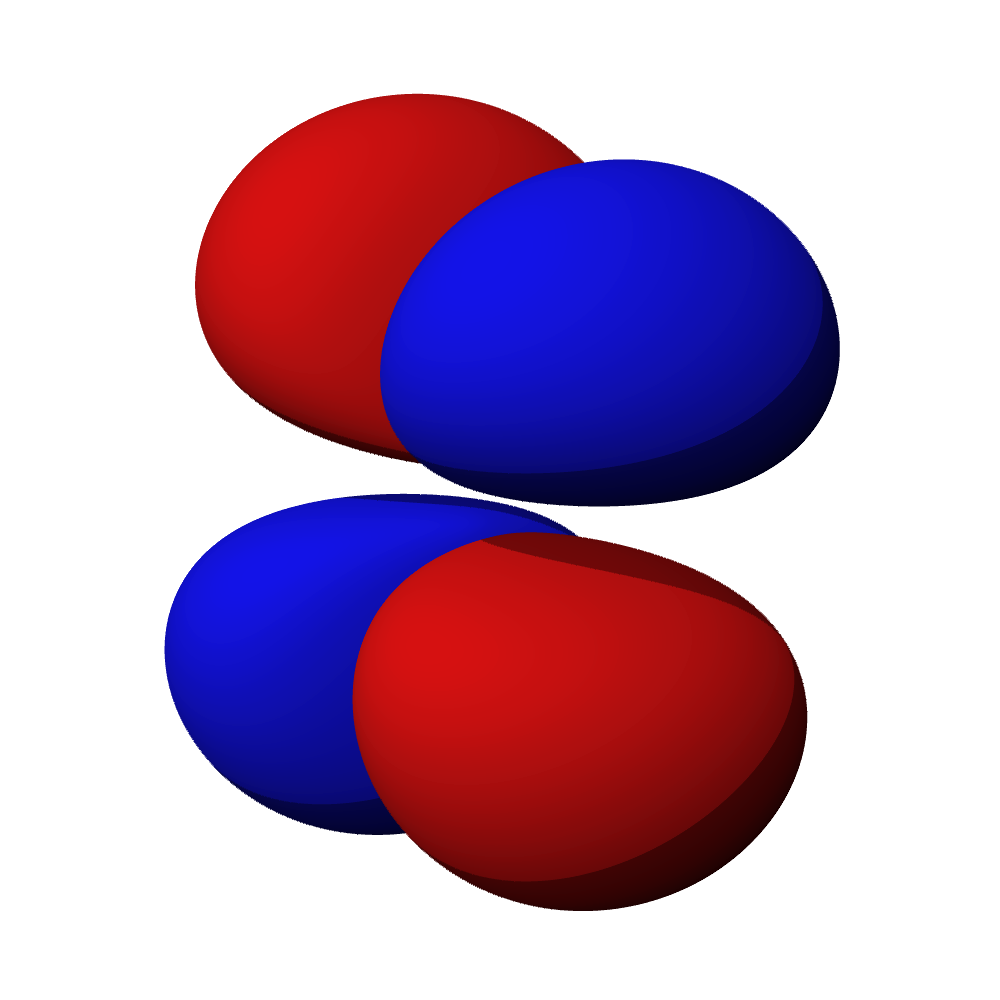
\includegraphics[width=1.6cm]{tableau_geometrie_orbitale_modelisation/Dyz_orbital.png} 
& 
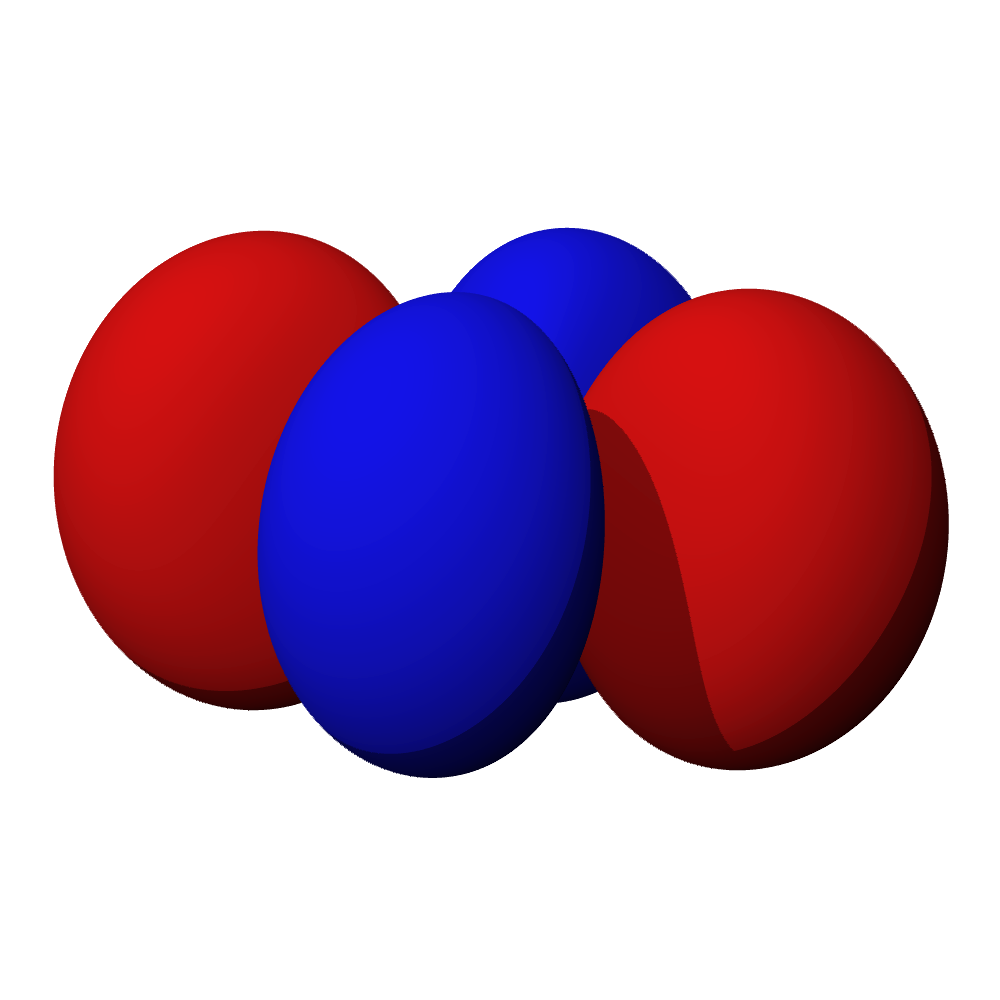
\includegraphics[width=1.6cm]{tableau_geometrie_orbitale_modelisation/Dxy_orbital.png} 
&
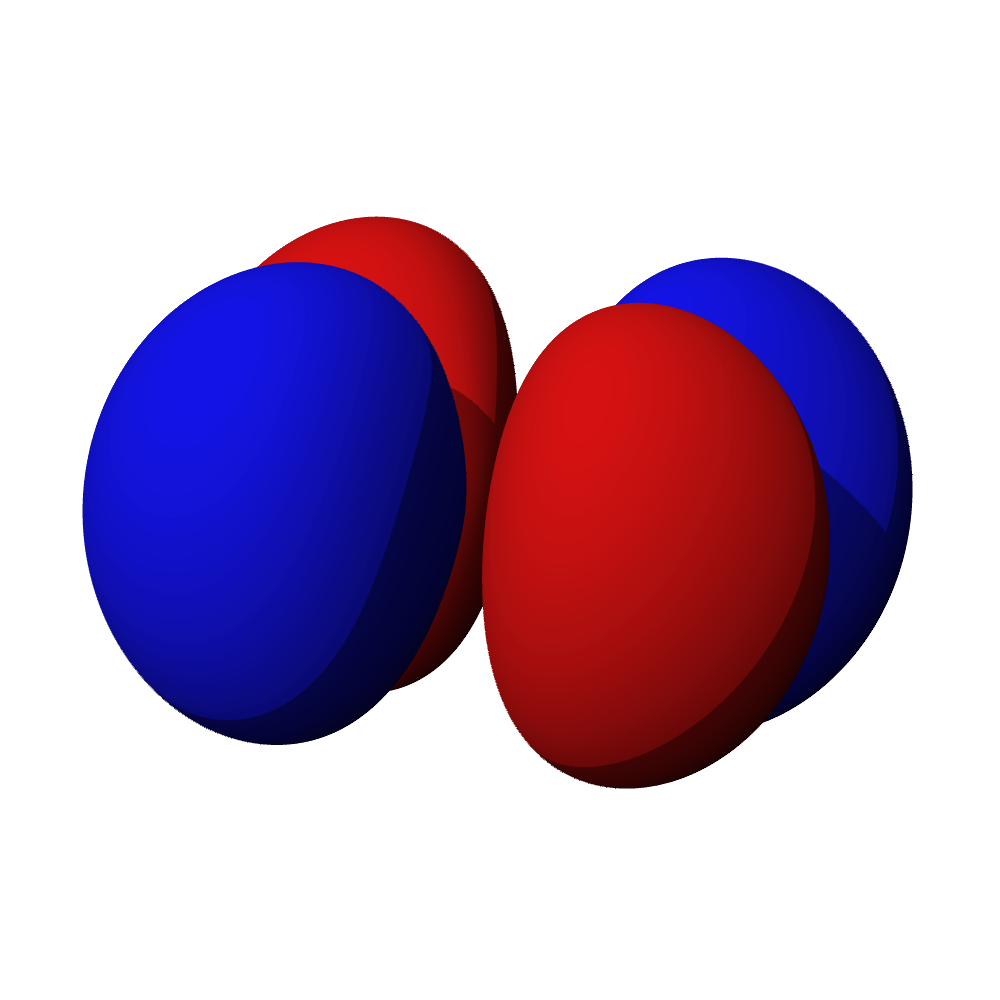
\includegraphics[width=1.6cm]{tableau_geometrie_orbitale_modelisation/Dx2-y2_orbital.png} 
& & \\
& & & \makecell[c]{$3d_{z^2}$} & \makecell[c]{$3d_{xz}$} & \makecell[c]{$3d_{yz}$} & \makecell[c]{$3d_{xy}$} & \makecell[c]{$3d_{x^{2}-y^{2}}$} & &  \\ %centrer la cellule individuellement 

\addlinespace

%\noalign{\break} %impose le saut de page au tableau tout en répartissant verticalement le tableau

\multirow[t]{8}{*}{$n=4$} & \multirow[t]{2}{*}{$\ell=0$} & \multirow[t]{2}{*}{$4s$} & 
\centering
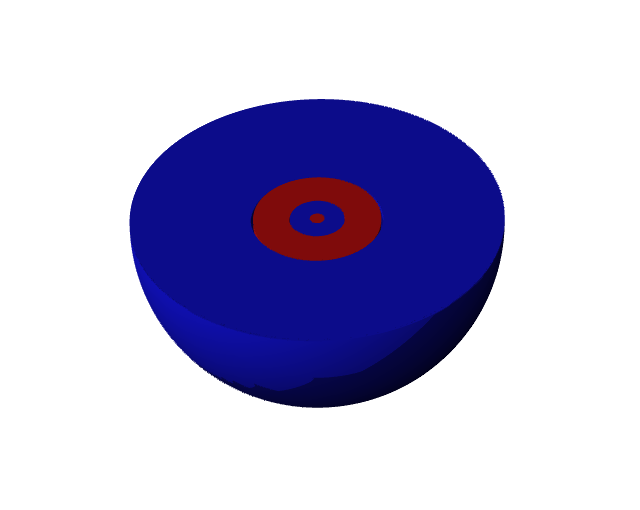
\includegraphics[width=1.6cm]{tableau_geometrie_orbitale_modelisation/S4M0.png} 
& & & & & & \\

& & & \makecell[c]{$3s$} & & & & & &  \\ %centrer la cellule individuellement 

\addlinespace

& \multirow[t]{2}{*}{$\ell=1$} & \multirow[t]{2}{*}{$4p$} & 
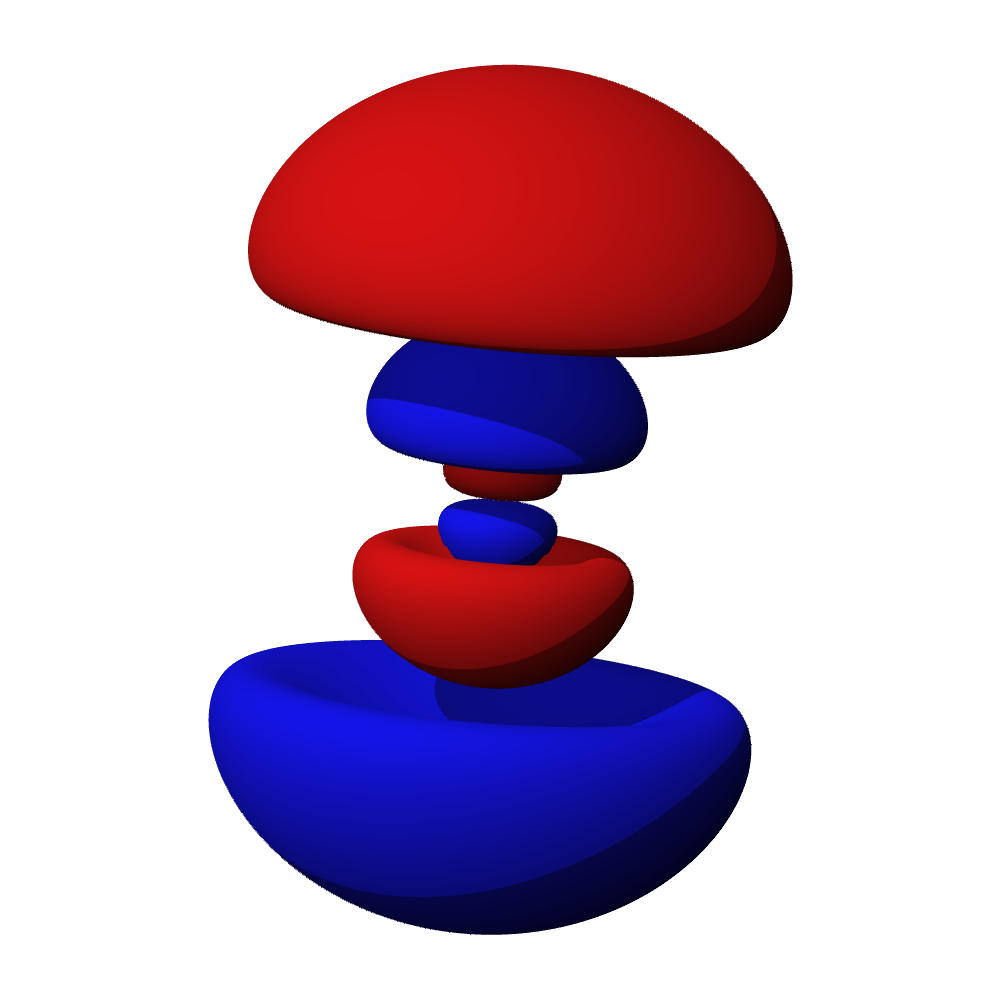
\includegraphics[width=1.6cm]{tableau_geometrie_orbitale_modelisation/P4z.png} 
&
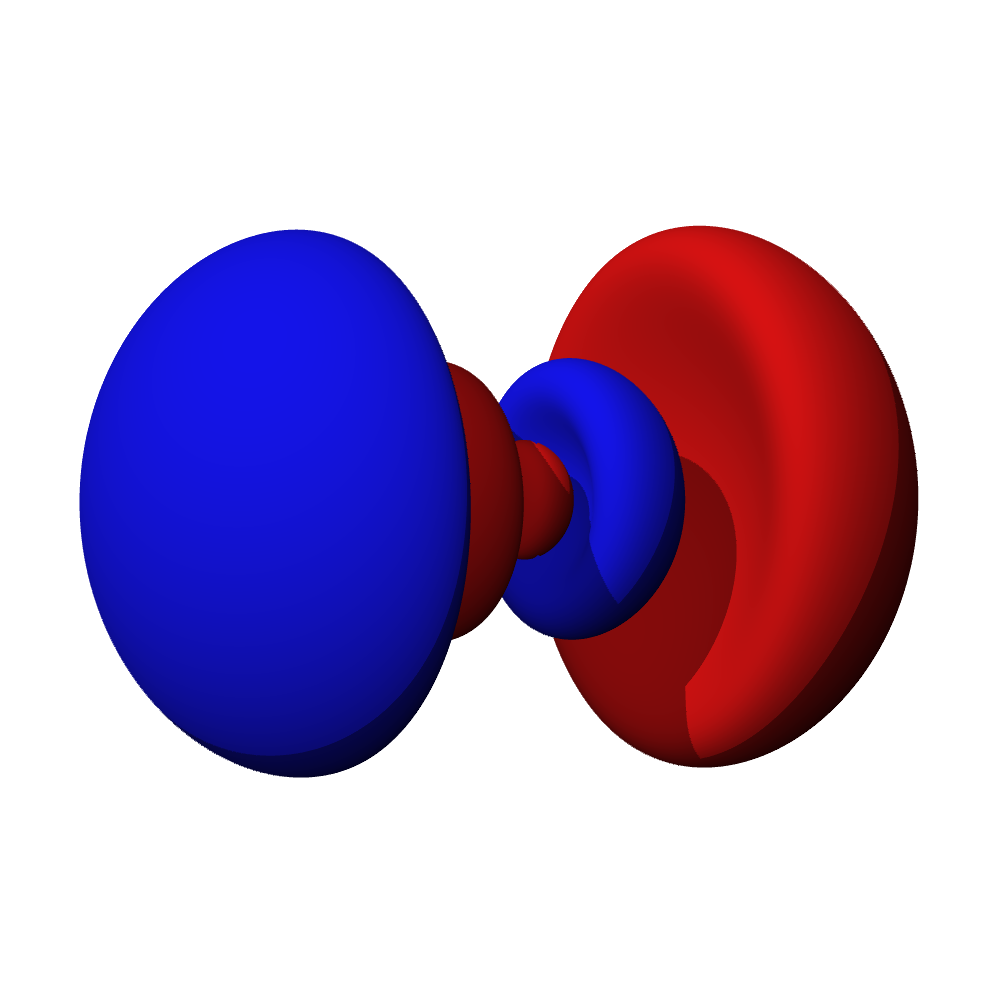
\includegraphics[width=1.6cm]{tableau_geometrie_orbitale_modelisation/P4x.png}  
&
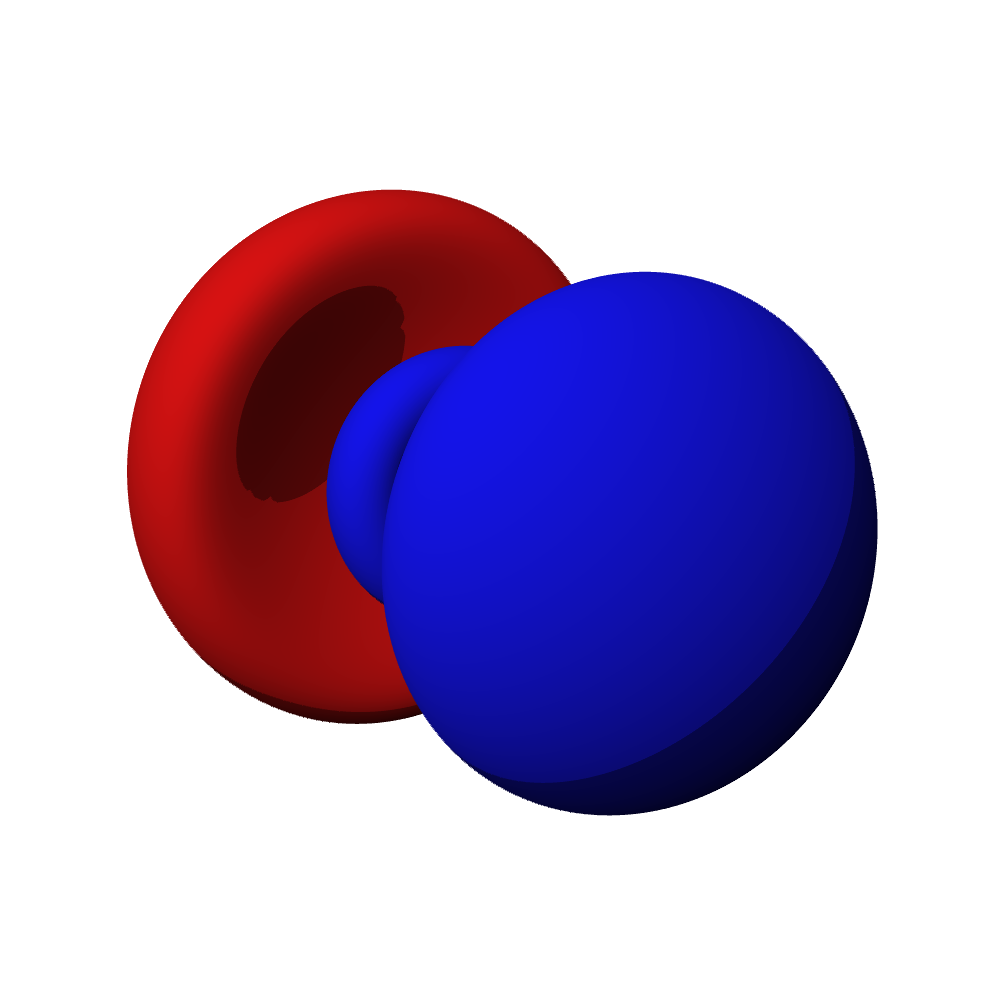
\includegraphics[width=1.6cm]{tableau_geometrie_orbitale_modelisation/P4y.png} 
& & & & \\

& & & \makecell[c]{$3p_z$} & \makecell[c]{$3p_x$} & \makecell[c]{$3p_y$} & & & &  \\ %centrer la cellule individuellement 

\addlinespace

& \multirow[t]{2}{*}{$\ell=2$} & \multirow[t]{2}{*}{$4d$} & 
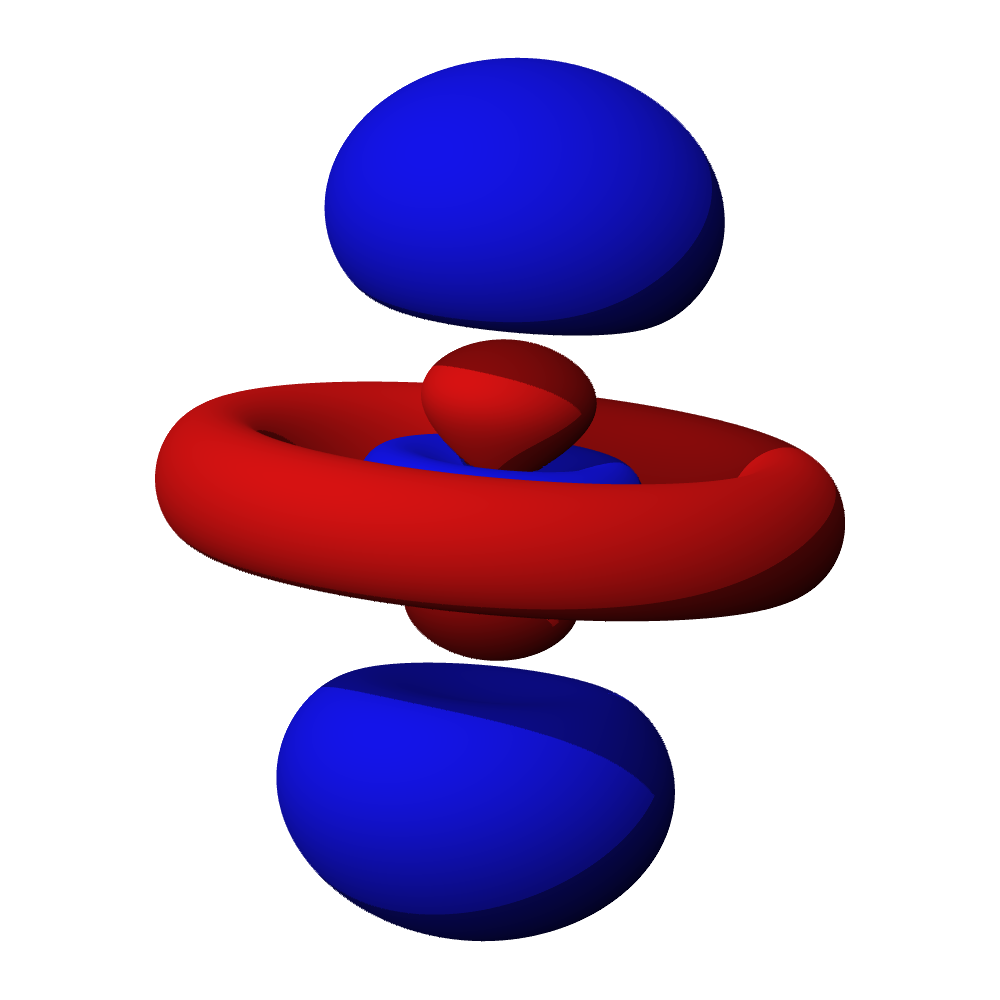
\includegraphics[width=1.6cm]{tableau_geometrie_orbitale_modelisation/D4z2.png} 
&
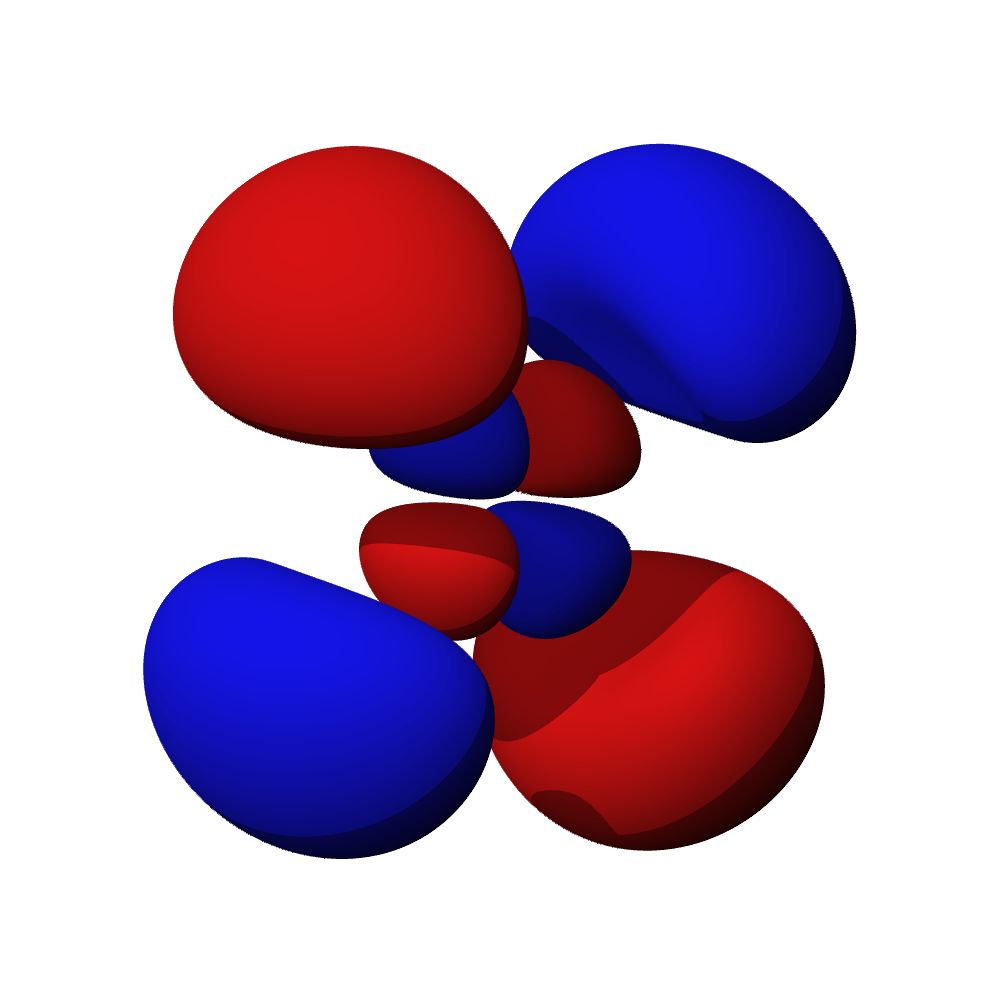
\includegraphics[width=1.6cm]{tableau_geometrie_orbitale_modelisation/D4xz.png}  
&
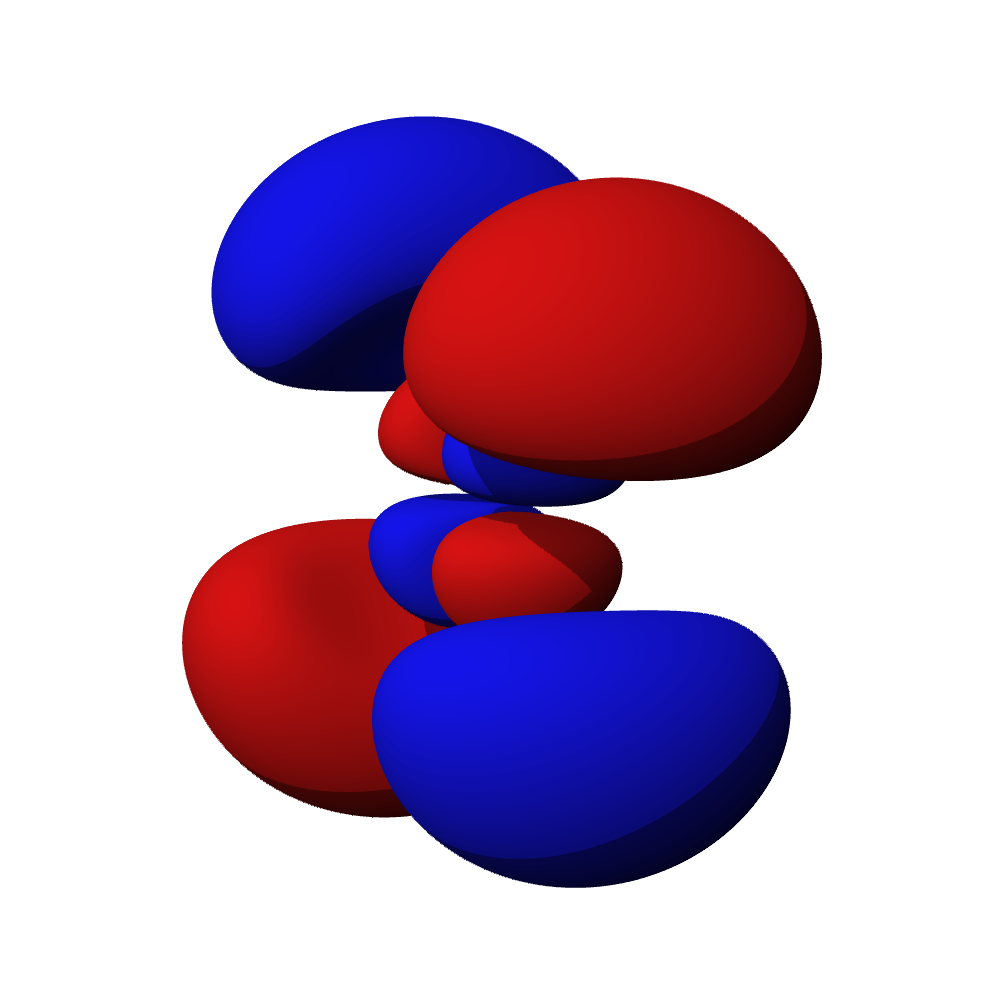
\includegraphics[width=1.6cm]{tableau_geometrie_orbitale_modelisation/D4yz.png} 
& 
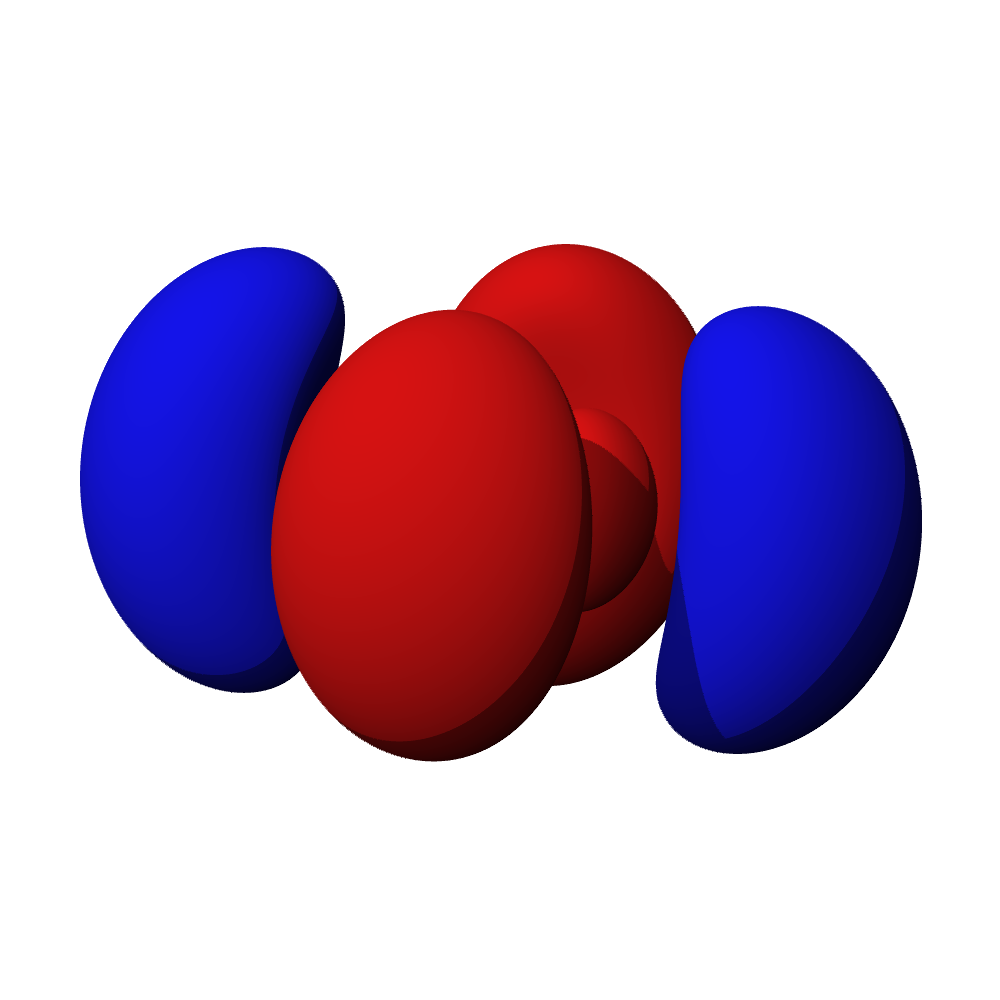
\includegraphics[width=1.6cm]{tableau_geometrie_orbitale_modelisation/D4xy.png} 
&
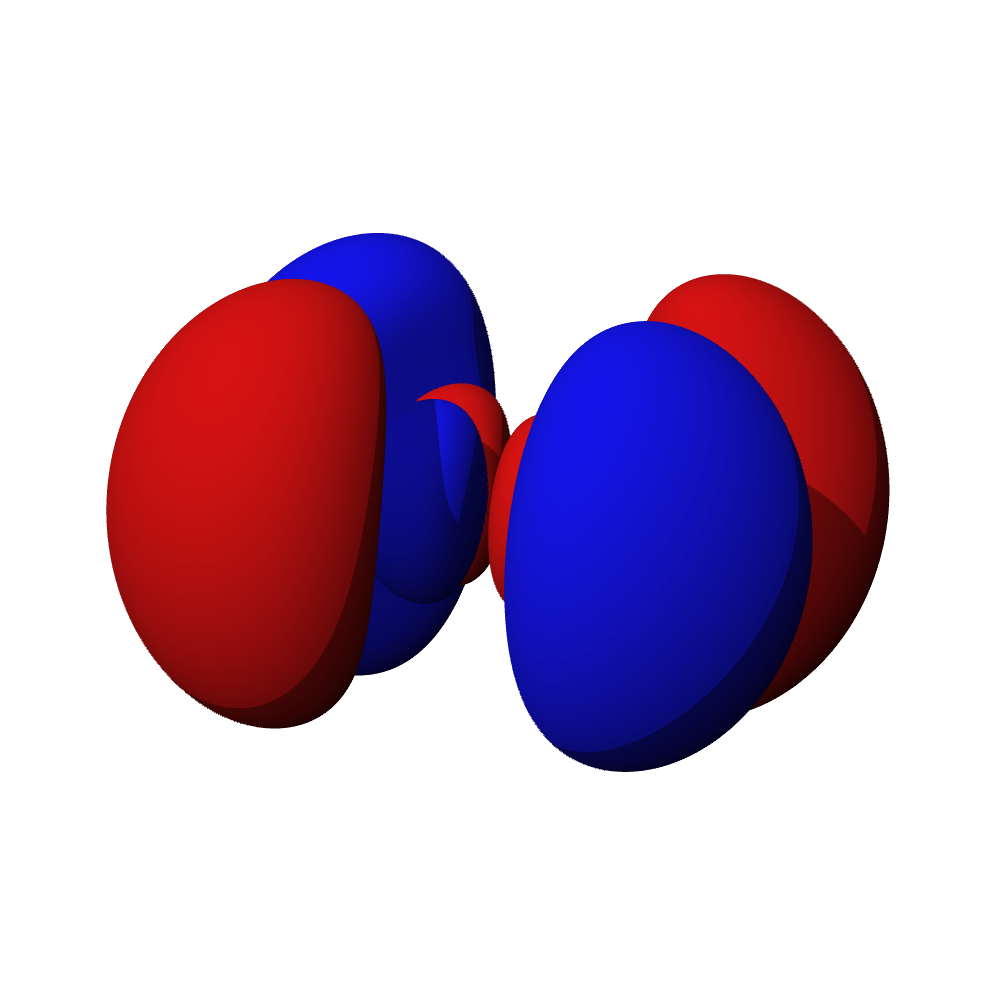
\includegraphics[width=1.6cm]{tableau_geometrie_orbitale_modelisation/D4x2-y2.png} 
& & \\

& & & \makecell[c]{$3d_{z^2}$} & \makecell[c]{$3d_{xz}$} & \makecell[c]{$3d_{yz}$} & \makecell[c]{$3d_{xy}$} & \makecell[c]{$3d_{x^{2}-y^{2}}$} & &  \\ %centrer la cellule individuellement 

\addlinespace

& \multirow[t]{2}{*}{$\ell=3$} & \multirow[t]{2}{*}{$4f$} & 
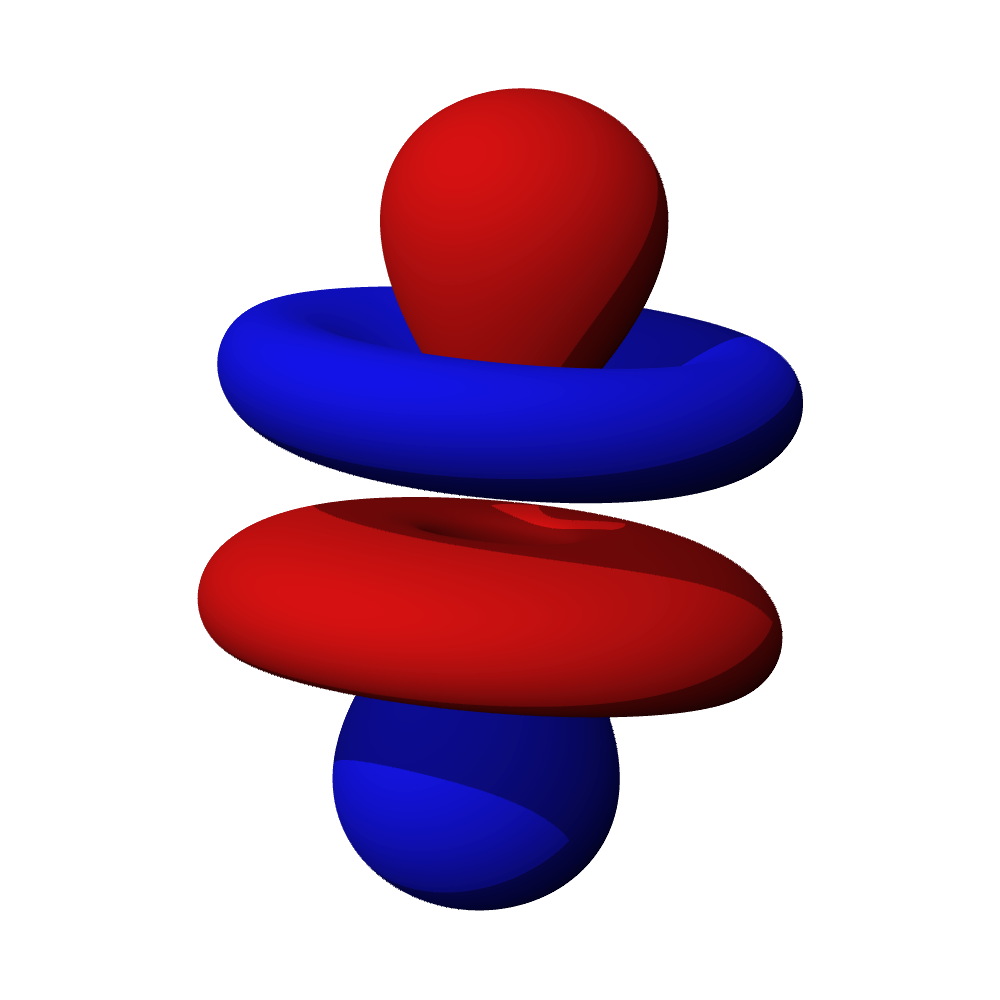
\includegraphics[width=1.6cm]{tableau_geometrie_orbitale_modelisation/Fz3_orbital.png} 
&
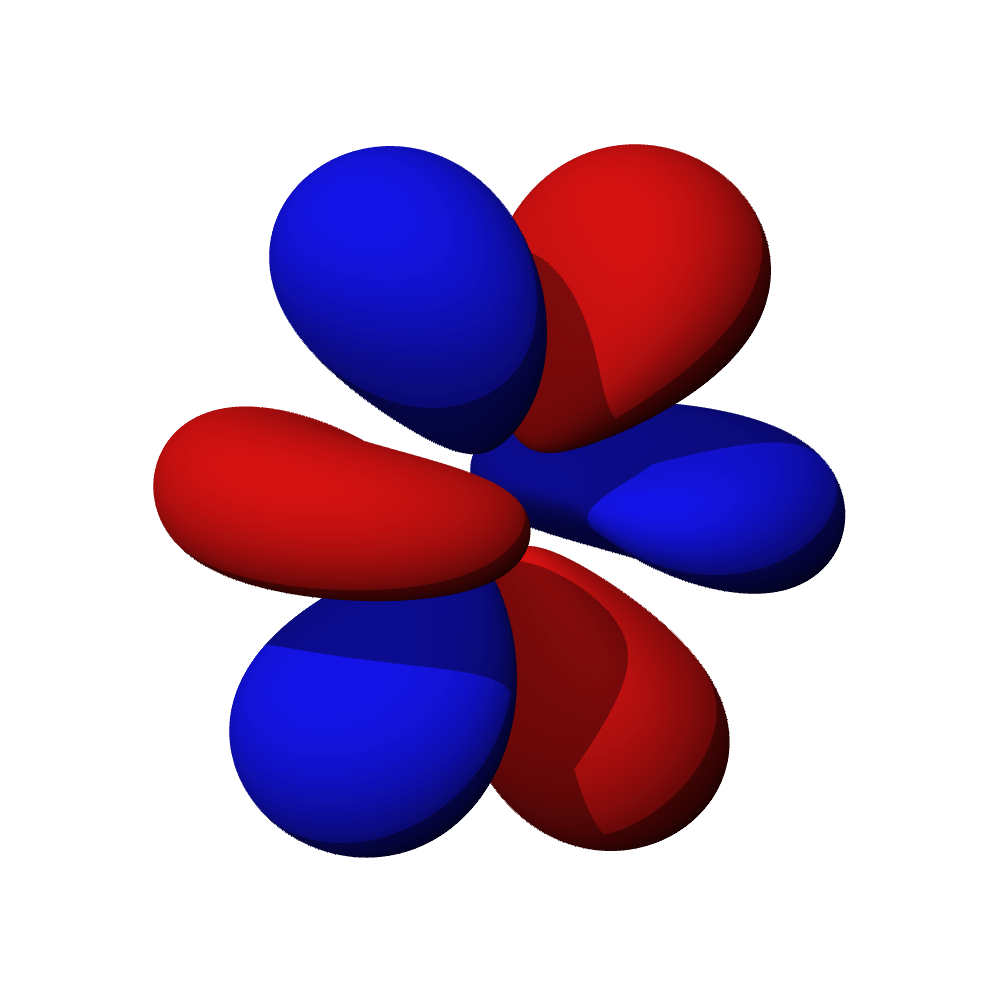
\includegraphics[width=1.6cm]{tableau_geometrie_orbitale_modelisation/Fxz2_orbital.png}  
&
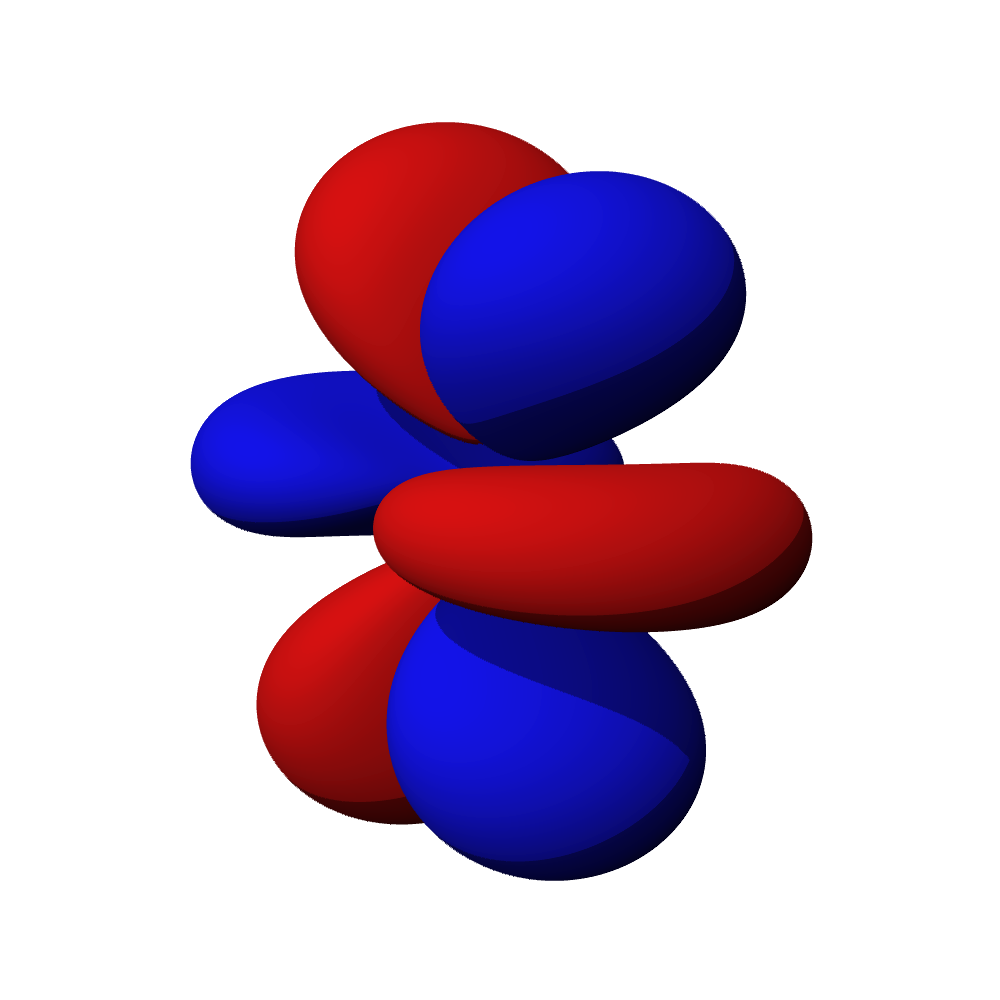
\includegraphics[width=1.6cm]{tableau_geometrie_orbitale_modelisation/Fyz2_orbital.png} 
& 
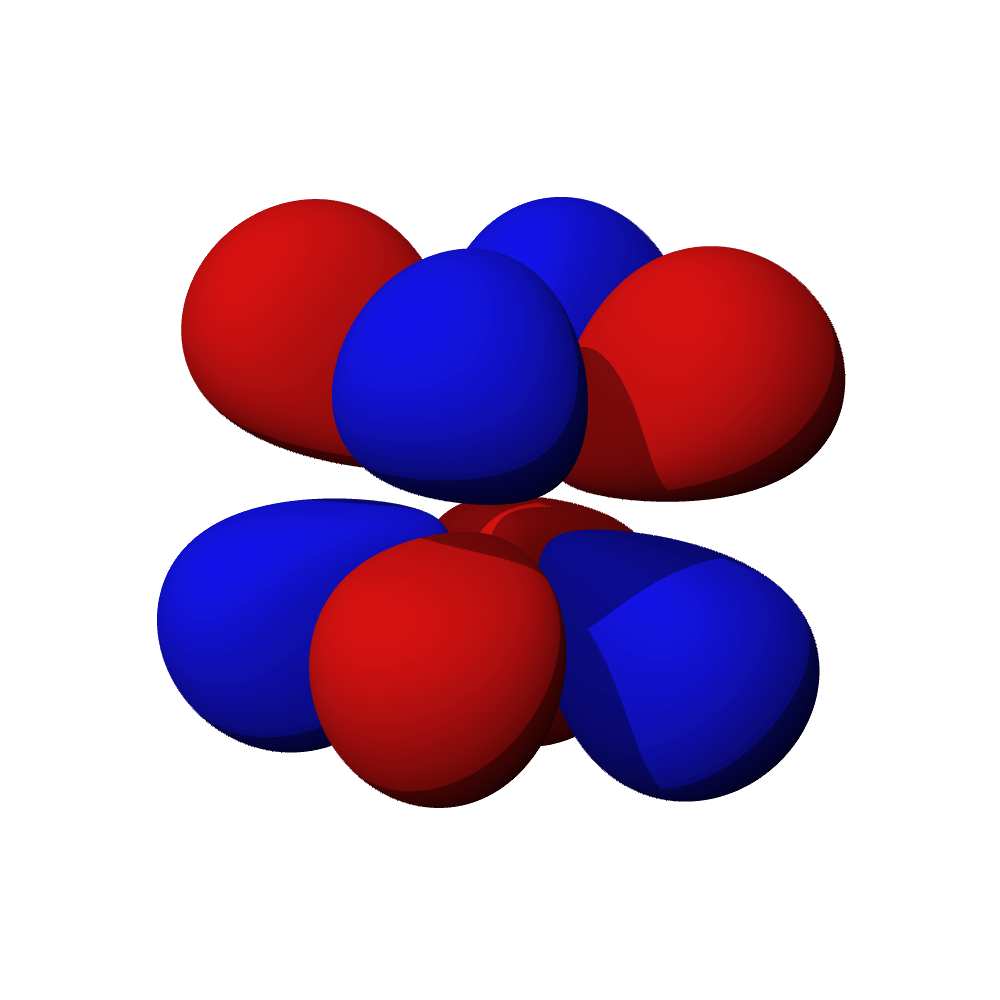
\includegraphics[width=1.6cm]{tableau_geometrie_orbitale_modelisation/Fxyz_orbital.png} 
&
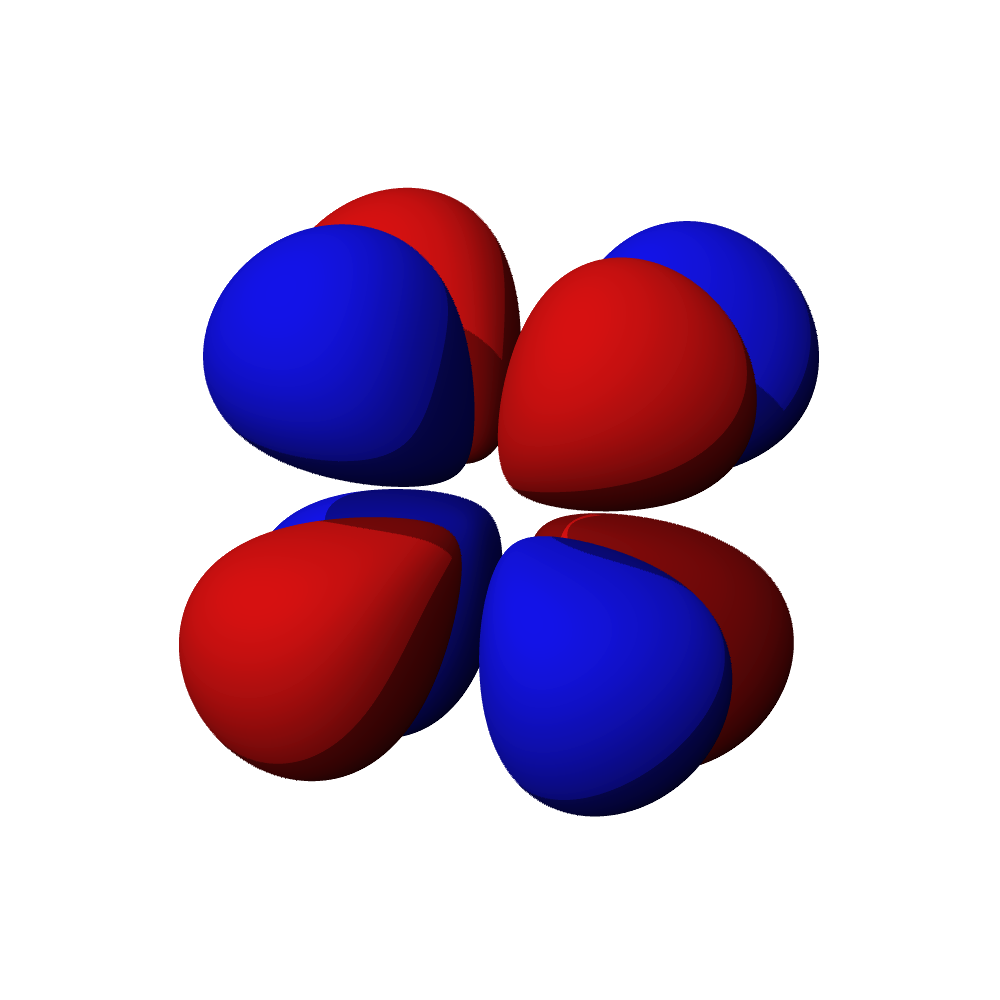
\includegraphics[width=1.6cm]{tableau_geometrie_orbitale_modelisation/Fz(x2-y2)_orbital.png} 
& 
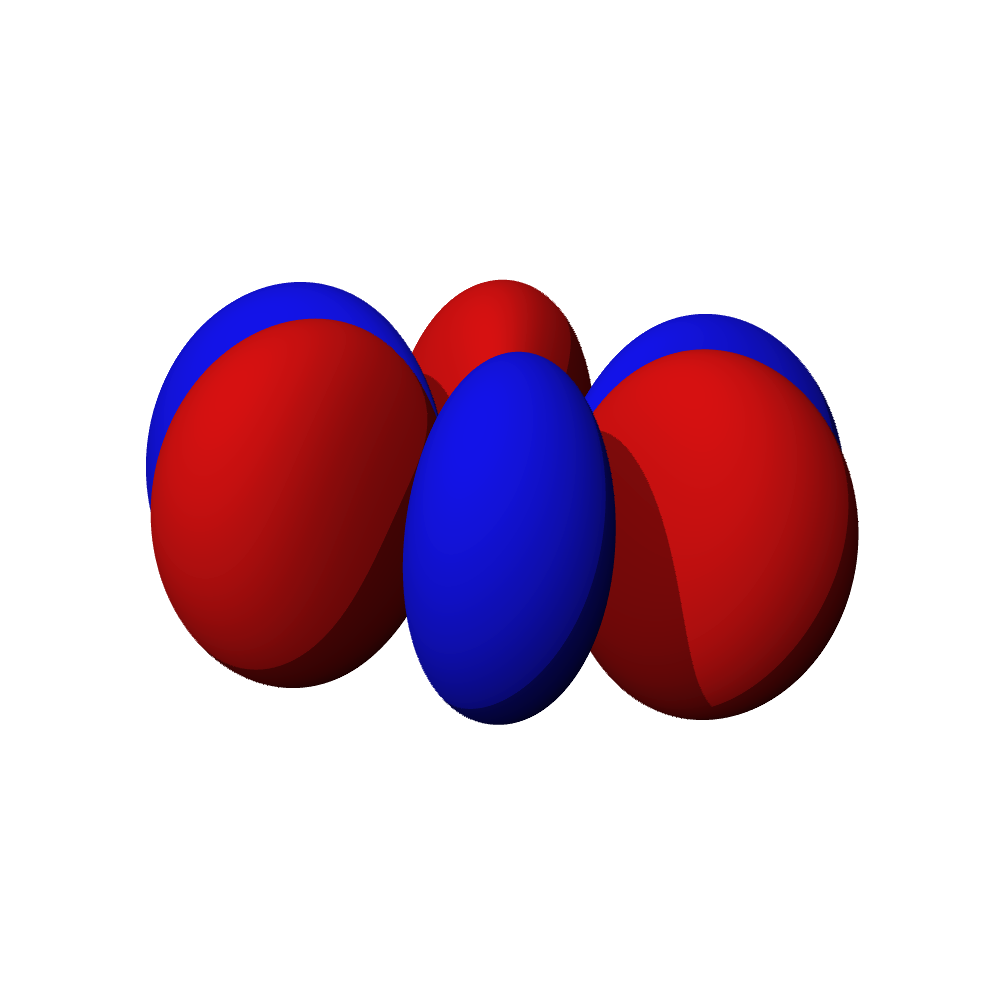
\includegraphics[width=1.6cm]{tableau_geometrie_orbitale_modelisation/Fx(x2-3y2)_orbital.png}
&
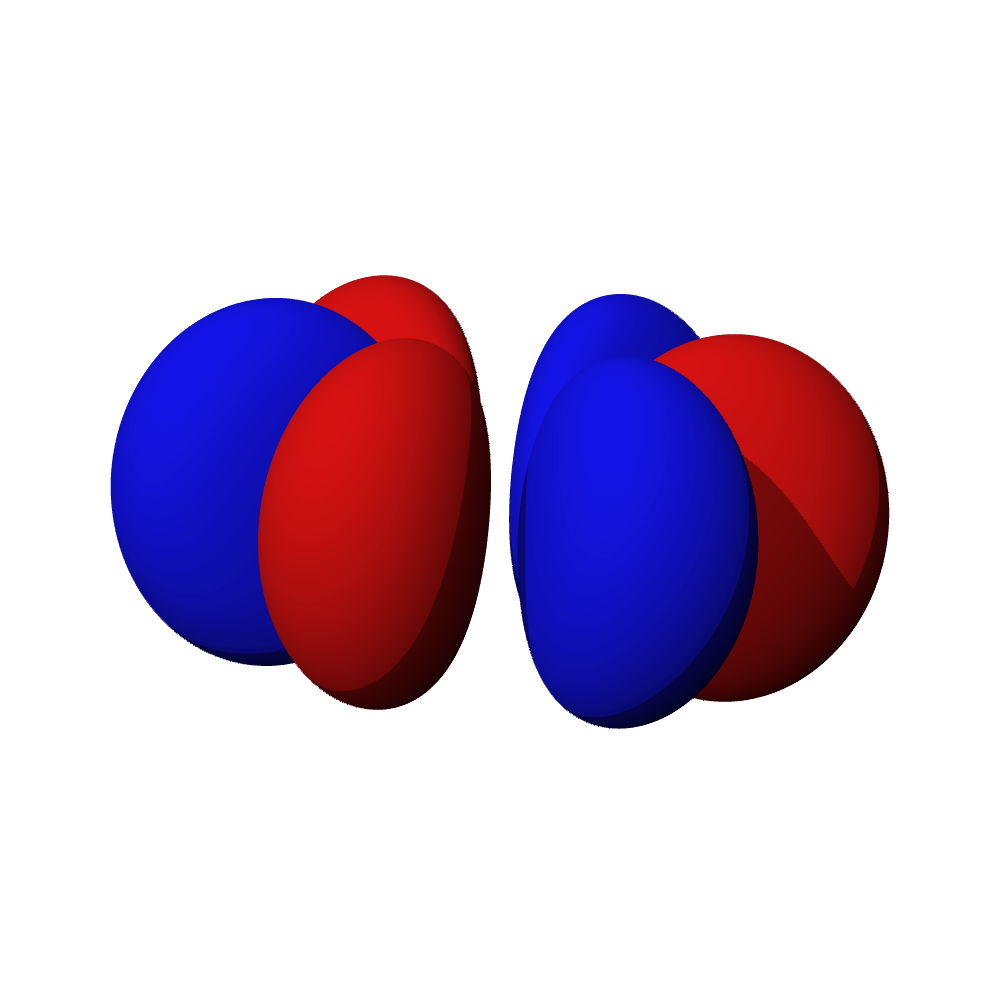
\includegraphics[width=1.6cm]{tableau_geometrie_orbitale_modelisation/Fy(3x2-y2)_orbital.png} \\

& & & \makecell[c]{$4f_{z^3}$} & \makecell[c]{$4f_{xz^2}$} & \makecell[c]{$4f_{yz^2}$} & \makecell[c]%
{$4f_{xyz}$} & \makecell[c]{$4f_{z(x^{2}-y^2)}$} & \makecell[c]{$4f_{x(x^{2}-y^2)}$} & \makecell[c]%
{$4f_{y(x^{2}-y^2)}$} \\ %centrer la cellule individuellement 

\midrule %filet de milieu de tableau

\multirow[t]{4}{*}{$n=5$} & \multirow[t]{2}{*}{$\ell=0$} & \multirow[t]{2}{*}{$5s$} & 
\centering
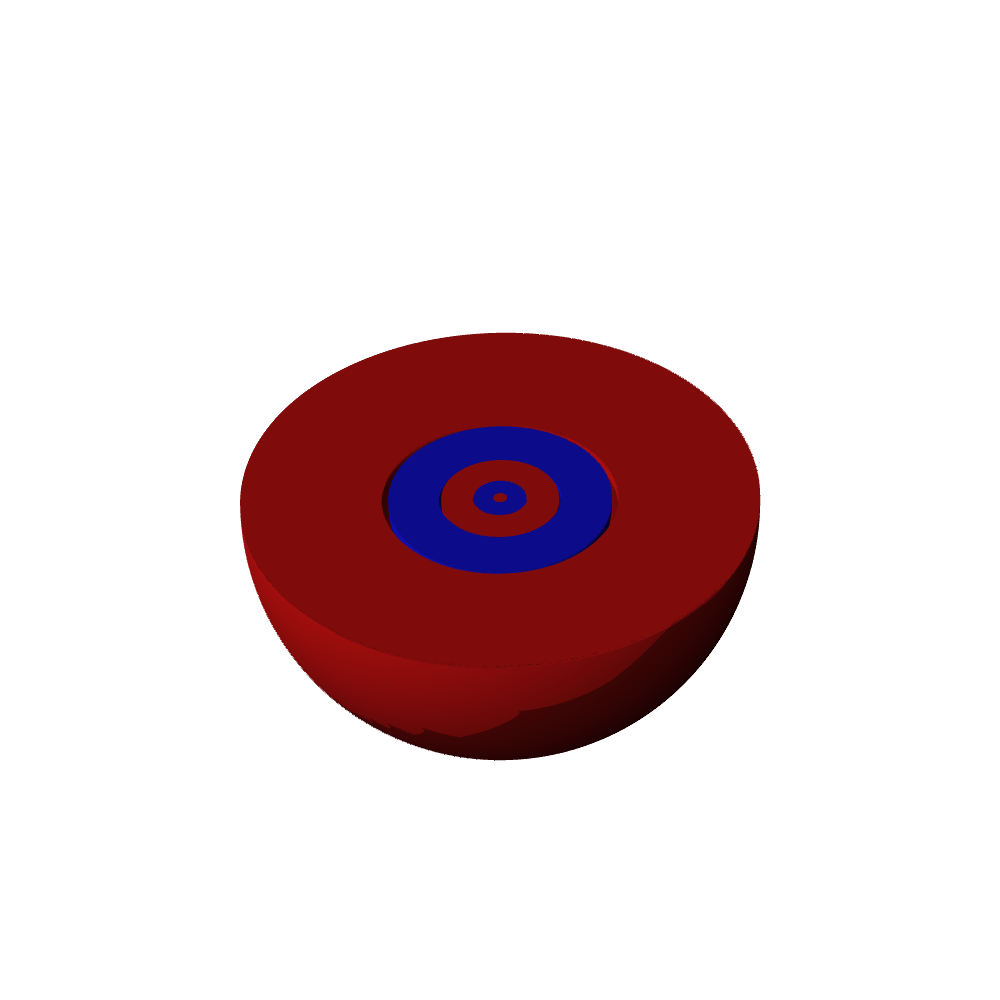
\includegraphics[width=1.6cm]{tableau_geometrie_orbitale_modelisation/S5M0.png} 
& & & & & & \\

& & & \makecell[c]{$5s$} & & & & & &  \\ %centrer la cellule individuellement 

\addlinespace

& \multirow[t]{2}{*}{$\ell=1$} & \multirow[t]{2}{*}{$5p$} & 
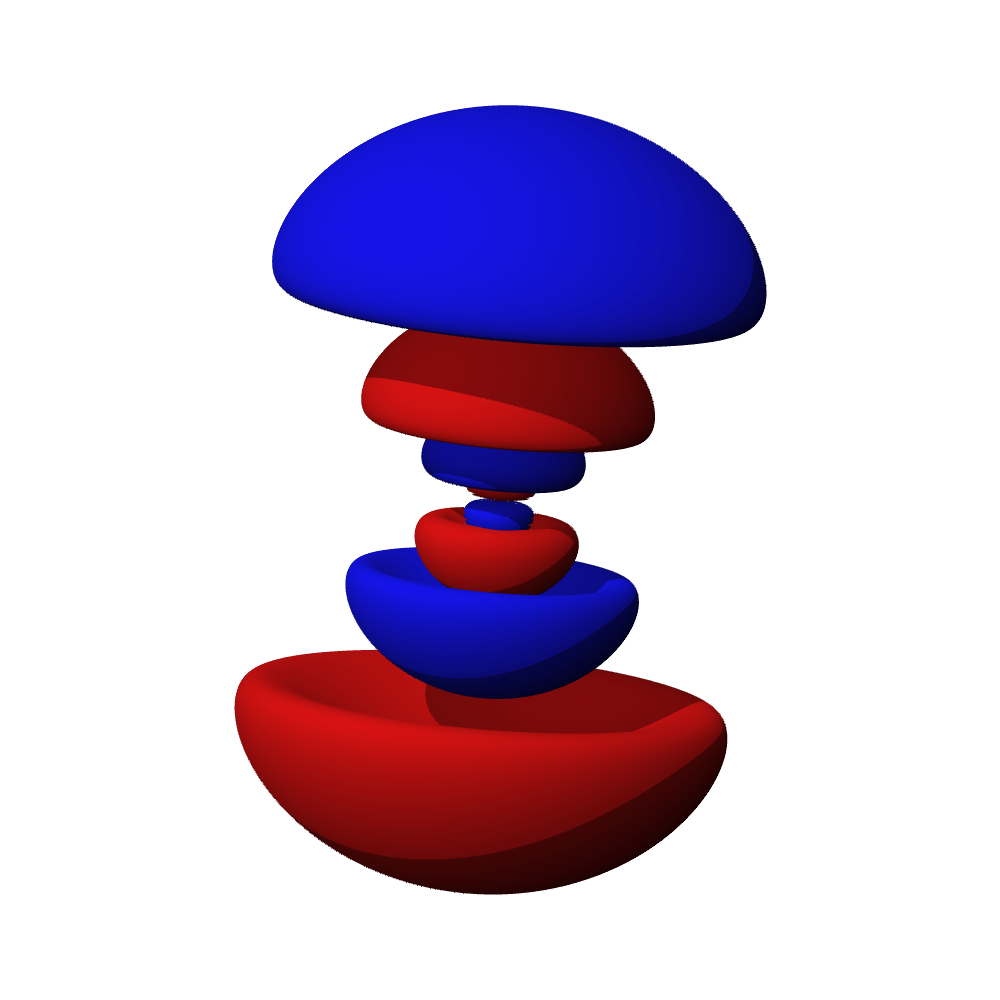
\includegraphics[width=1.6cm]{tableau_geometrie_orbitale_modelisation/P5z.png} 
&
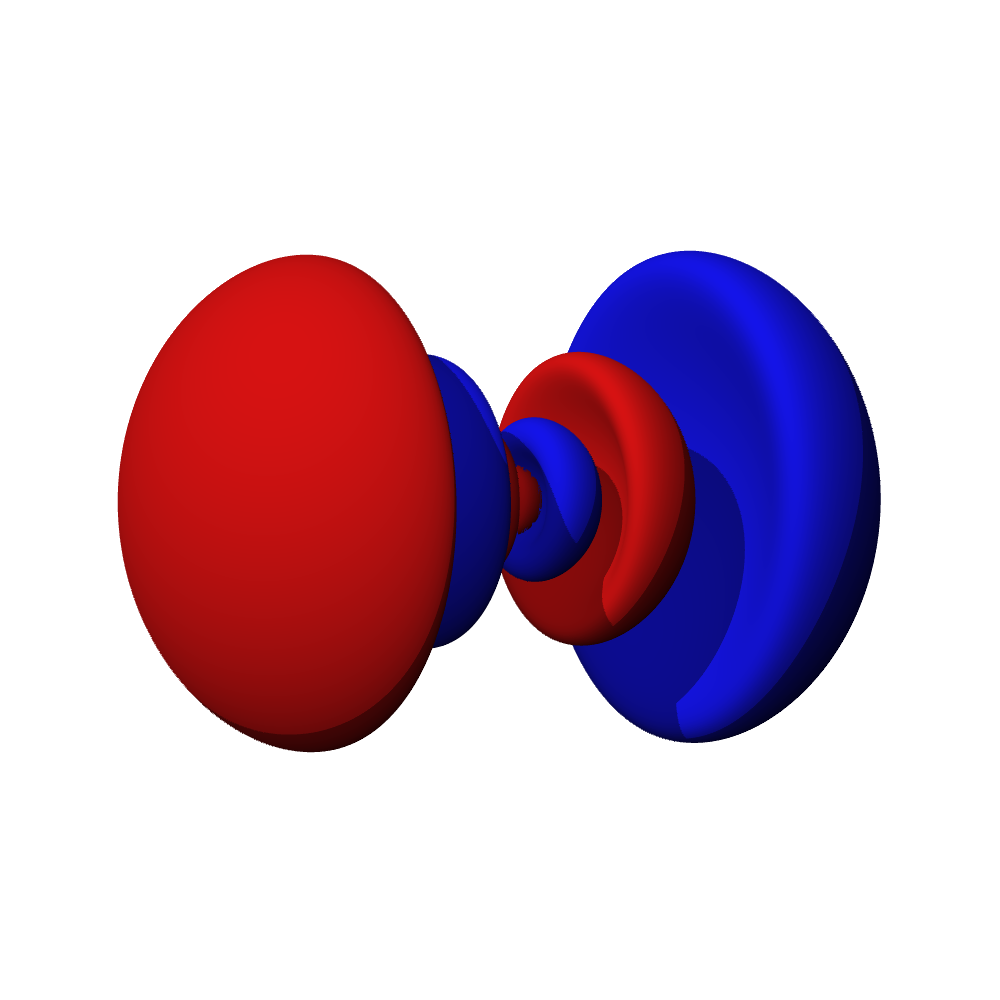
\includegraphics[width=1.6cm]{tableau_geometrie_orbitale_modelisation/P5x.png}  
&
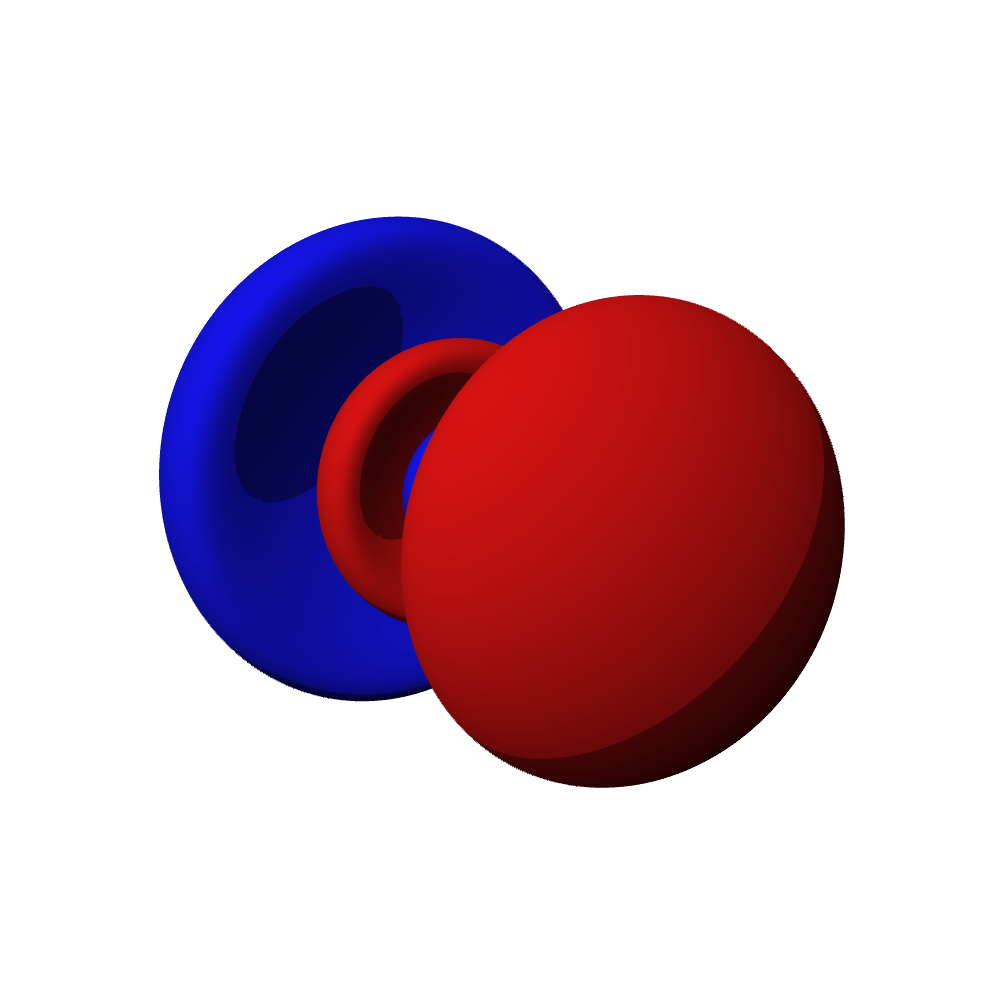
\includegraphics[width=1.6cm]{tableau_geometrie_orbitale_modelisation/P5y.png} 
& & & & \\

& & & \makecell[c]{$5p_z$} & \makecell[c]{$5p_x$} & \makecell[c]{$5p_y$} & & & &  \\ %centrer la cellule individuellement 

\addlinespace

\multirow[t]{2}{*}{$n=5$} & \multirow[t]{2}{*}{$\ell=2$} & \multirow[t]{2}{*}{$5d$} & 
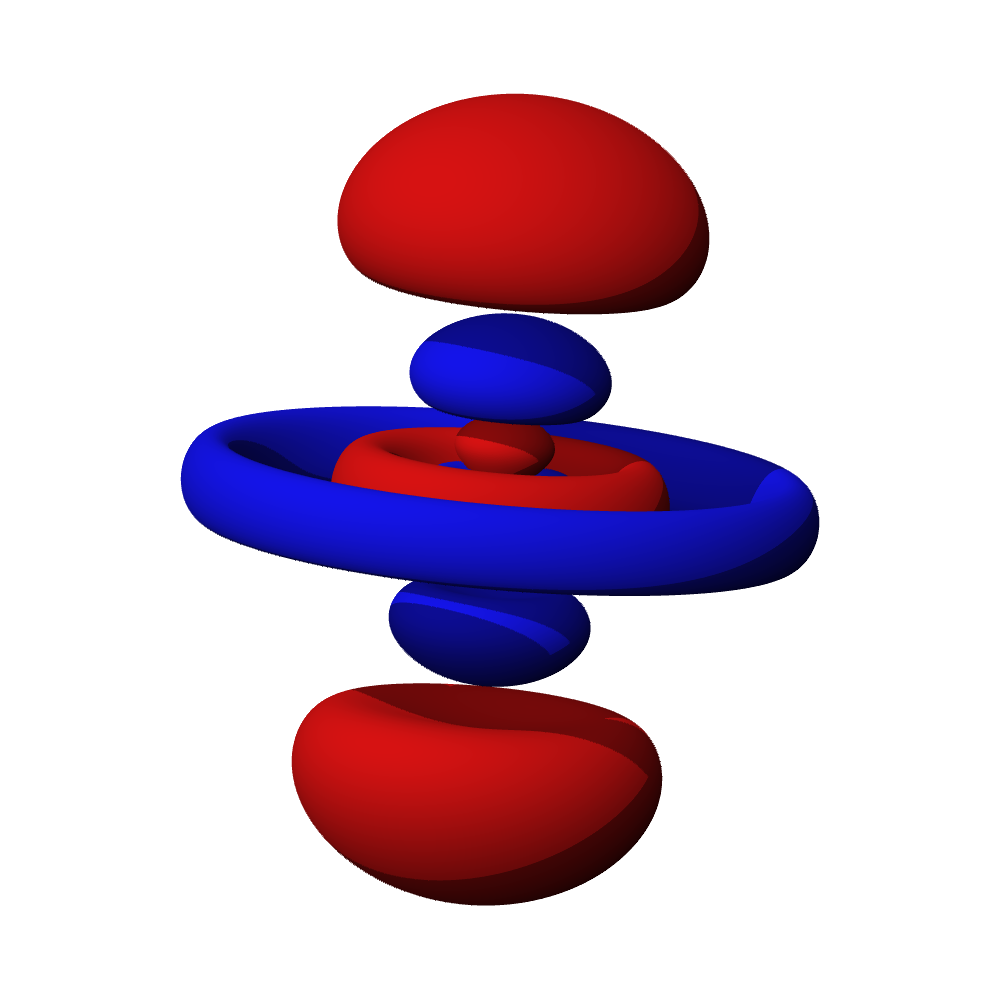
\includegraphics[width=1.6cm]{tableau_geometrie_orbitale_modelisation/D5z2.png} 
&
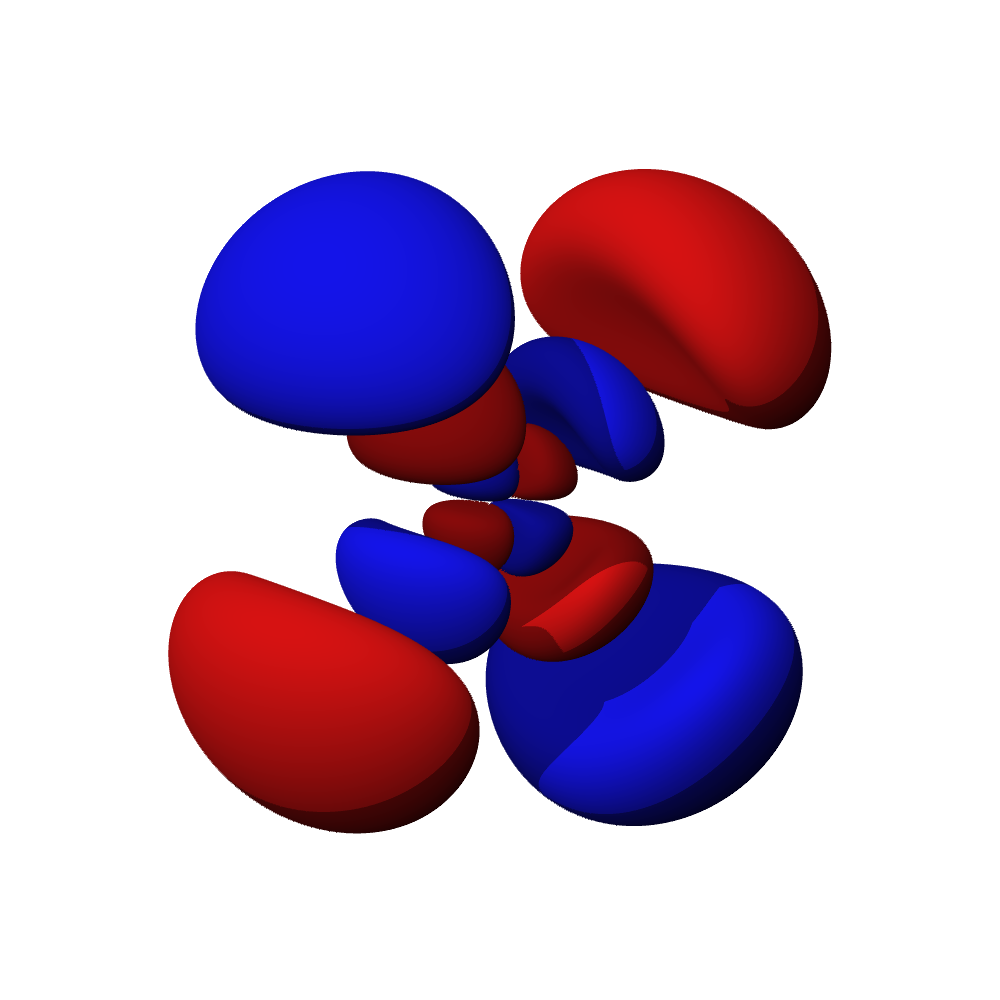
\includegraphics[width=1.6cm]{tableau_geometrie_orbitale_modelisation/D5xz.png}  
&
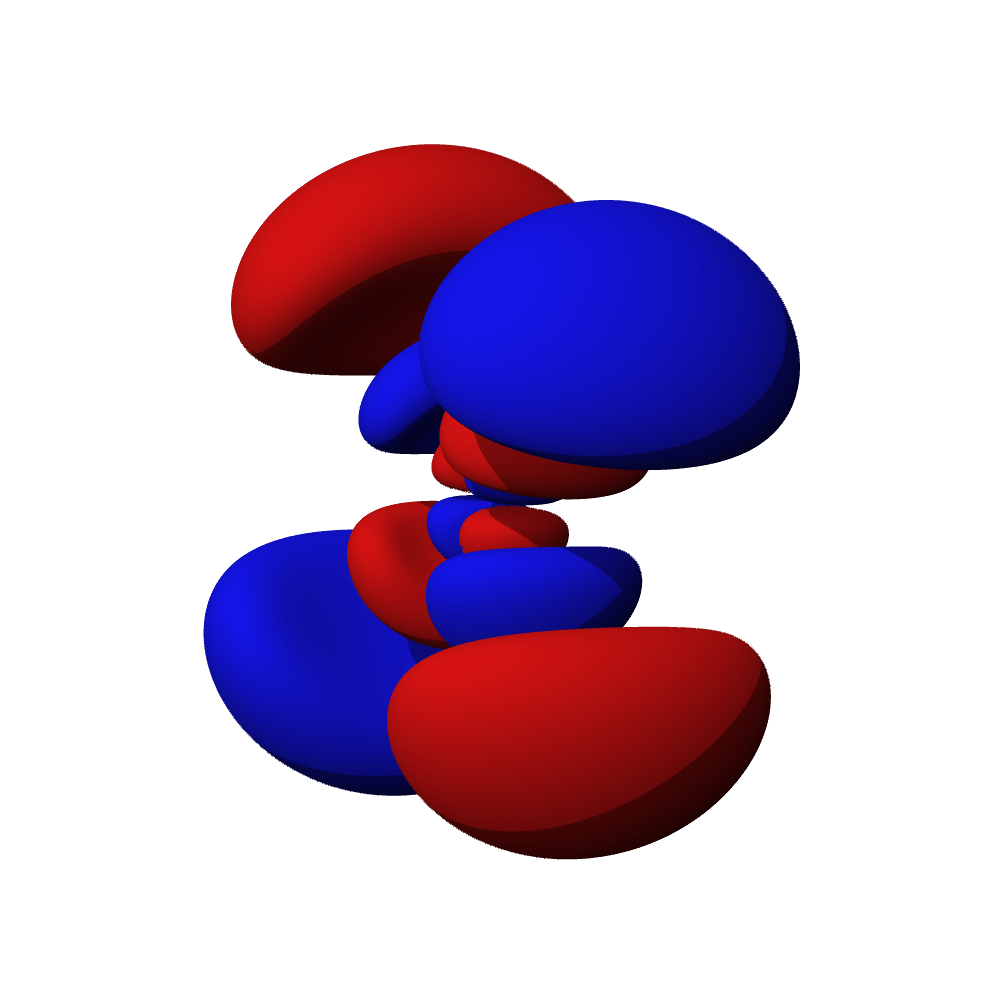
\includegraphics[width=1.6cm]{tableau_geometrie_orbitale_modelisation/D5yz.png} 
& 
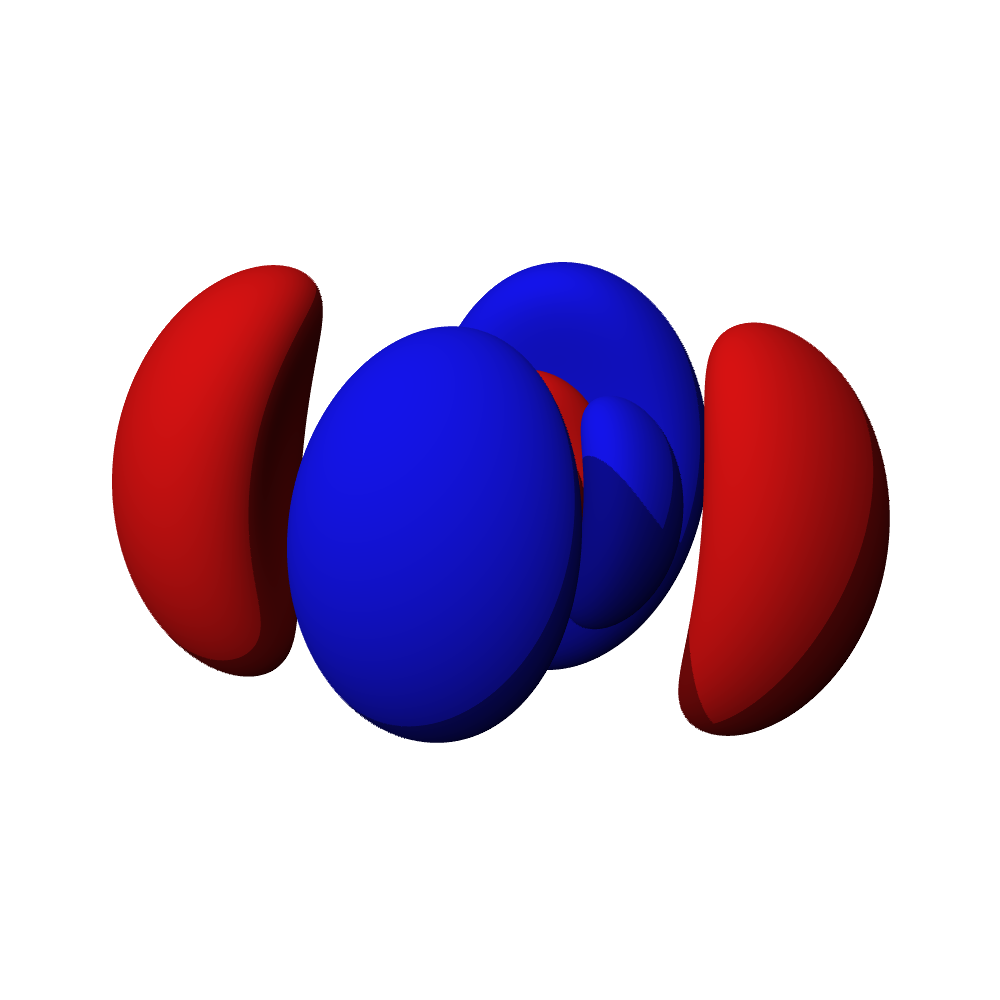
\includegraphics[width=1.6cm]{tableau_geometrie_orbitale_modelisation/D5xy.png} 
&
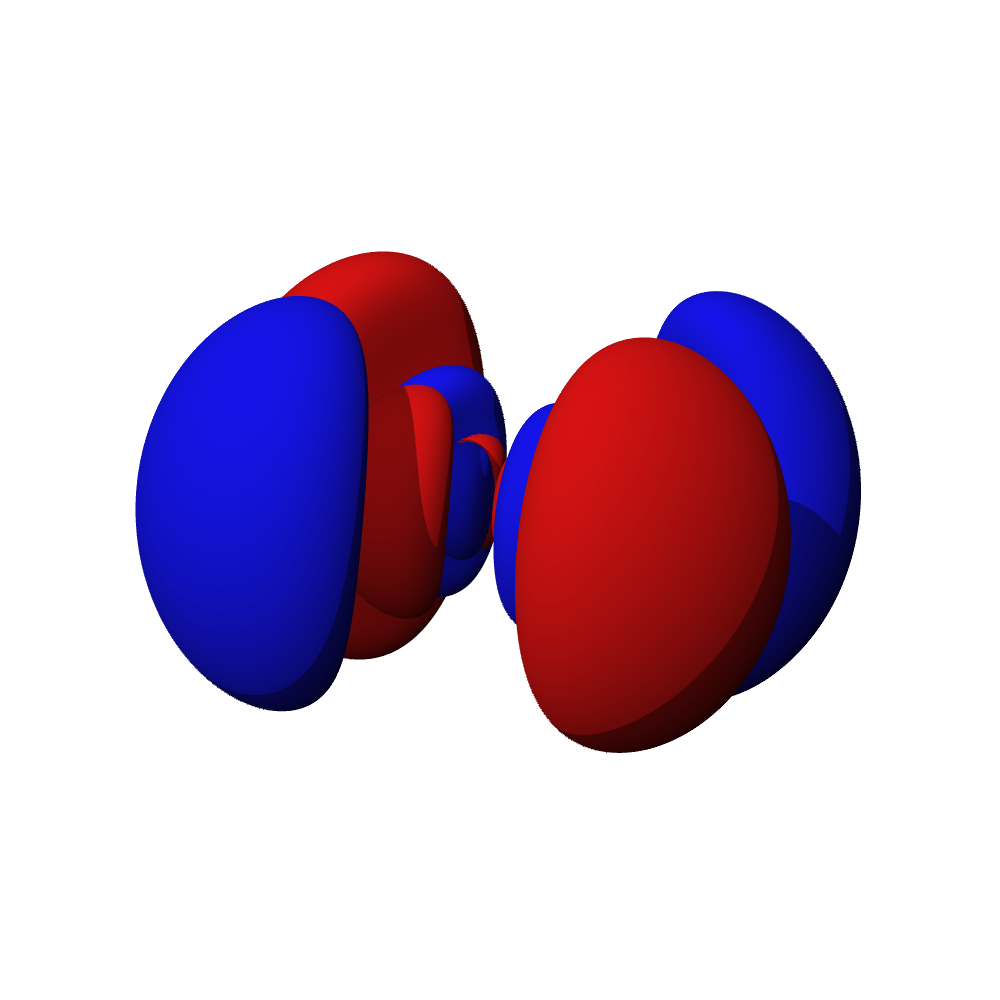
\includegraphics[width=1.6cm]{tableau_geometrie_orbitale_modelisation/D5x2-y2.png} 
& & \\
& & & \makecell[c]{$5d_{z^2}$} & \makecell[c]{$5d_{xz}$} & \makecell[c]{$5d_{yz}$} & \makecell[c]{$5d_{xy}$} & \makecell[c]{$5d_{x^{2}-y^{2}}$} & &  \\ %centrer la cellule individuellement 

\midrule

\multirow[t]{6}{*}{$n=6$} & \multirow[t]{2}{*}{$\ell=0$} & \multirow[t]{2}{*}{$6s$} & 
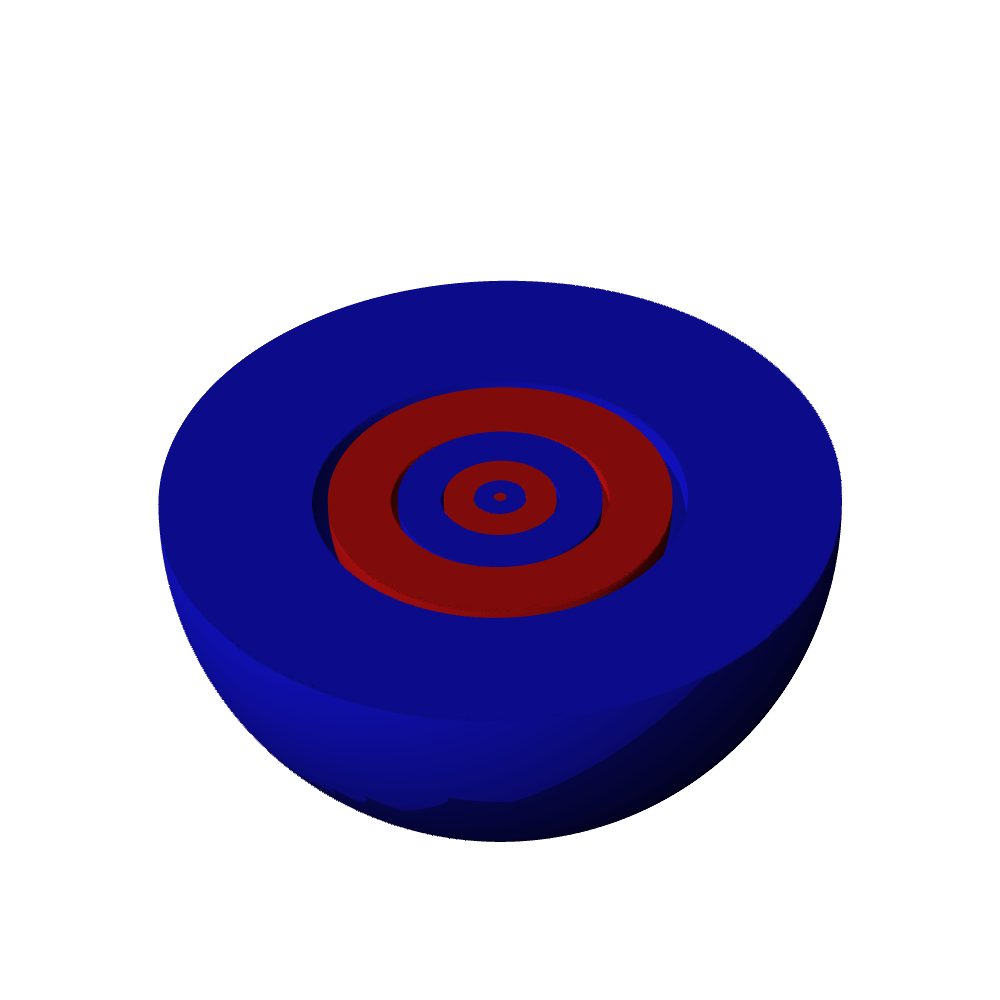
\includegraphics[width=1.6cm]{tableau_geometrie_orbitale_modelisation/S6M0.png} 
& & & & & & \\

& & & \makecell[c]{$6s$} & & & & & &  \\ %centrer la cellule individuellement 

\addlinespace

& \multirow[t]{2}{*}{$\ell=1$} & \multirow[t]{2}{*}{$6p$} & 
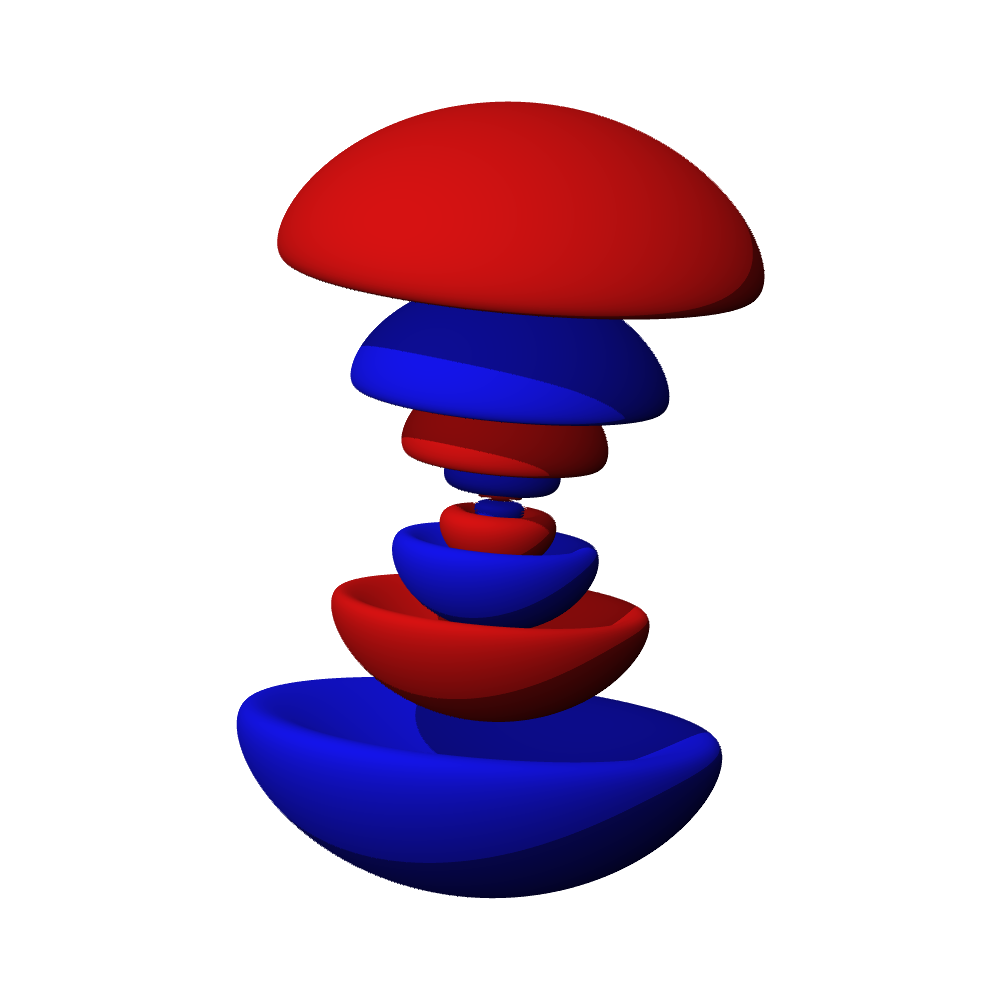
\includegraphics[width=1.6cm]{tableau_geometrie_orbitale_modelisation/P6z.png} 
&
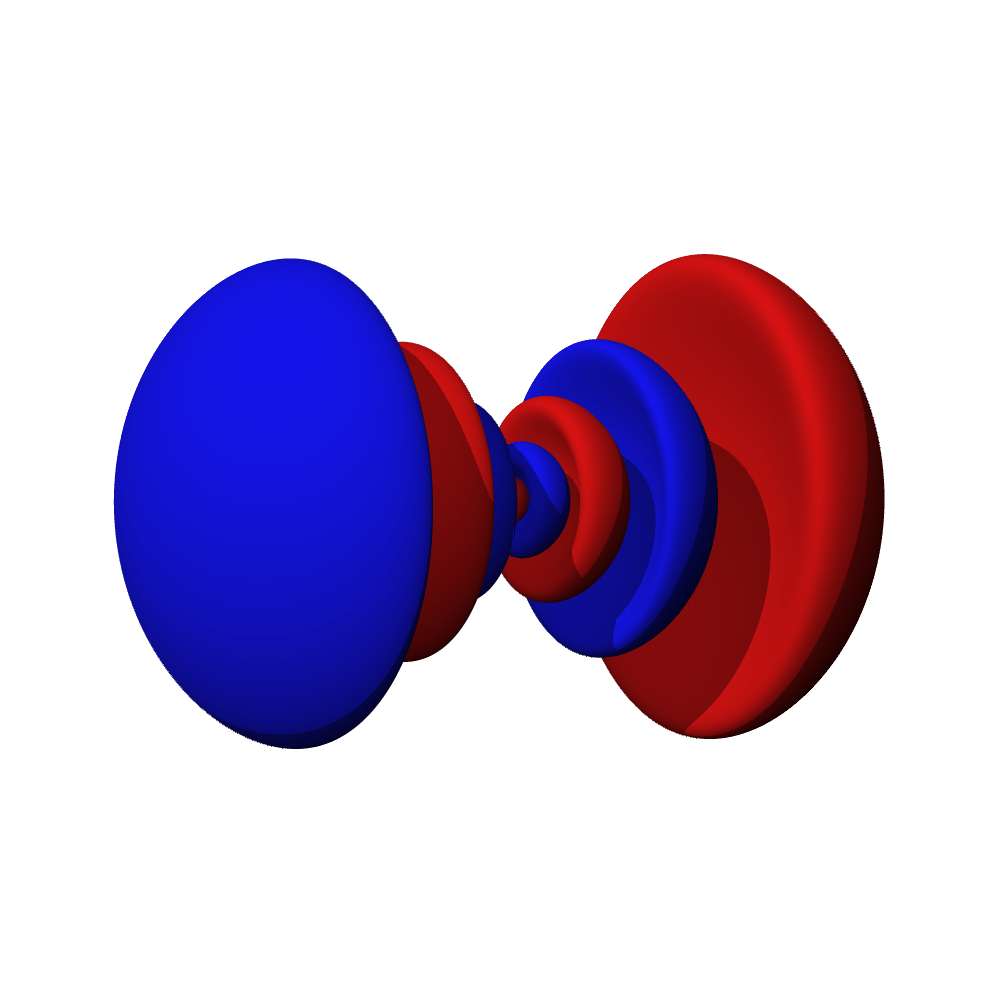
\includegraphics[width=1.6cm]{tableau_geometrie_orbitale_modelisation/P6x.png}  
&
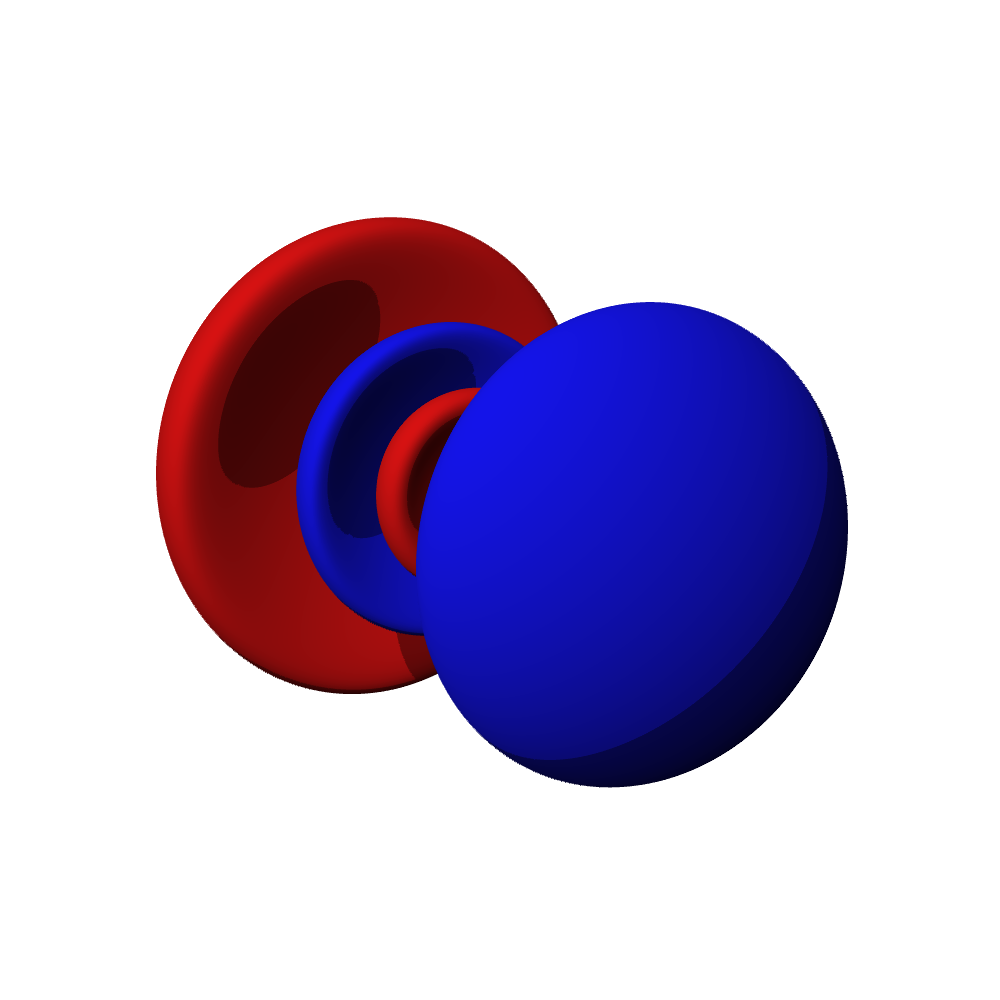
\includegraphics[width=1.6cm]{tableau_geometrie_orbitale_modelisation/P6y.png} 
& & & & \\

& & & \makecell[c]{$6p_z$} & \makecell[c]{$6p_x$} & \makecell[c]{$6p_y$} & & & &  \\ %centrer la cellule individuellement 

\addlinespace

 & \multirow[t]{2}{*}{$\ell=2$} & \multirow[t]{2}{*}{$6d$} & 
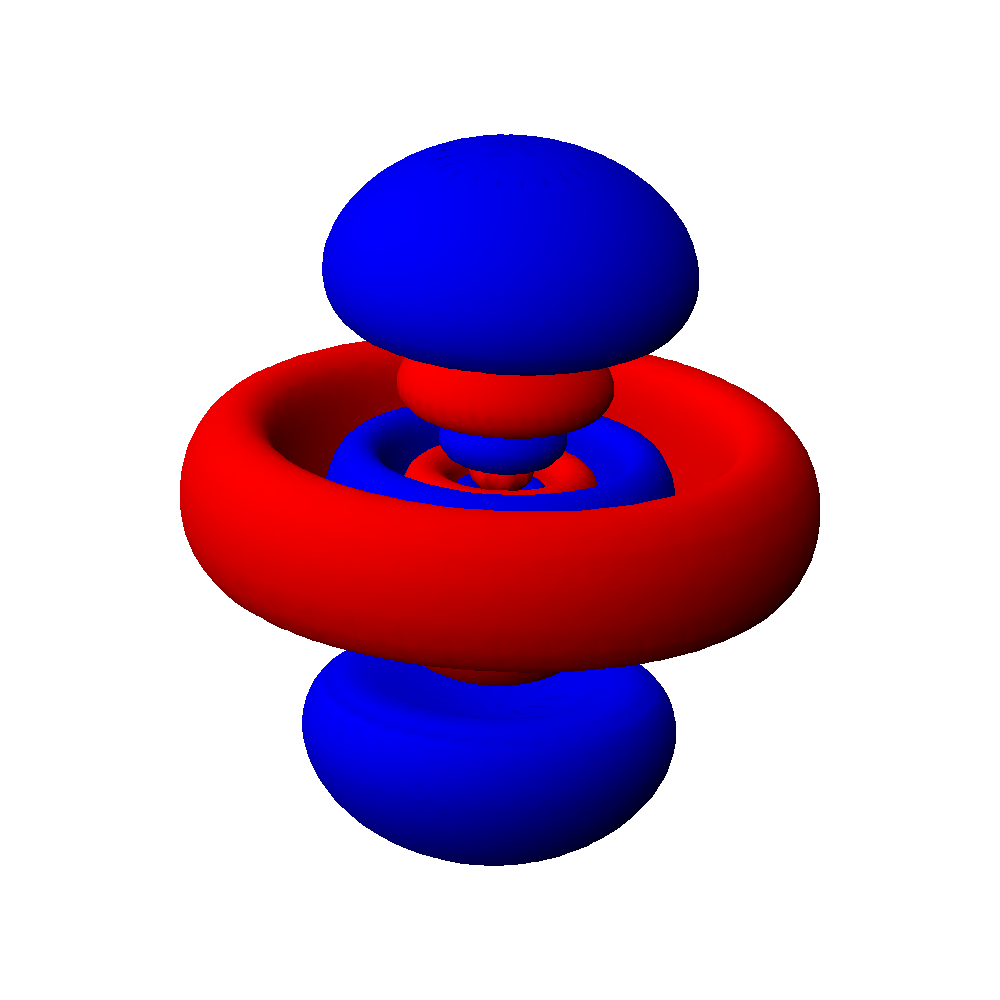
\includegraphics[width=1.6cm]{tableau_geometrie_orbitale_modelisation/D6z2.png} 
&
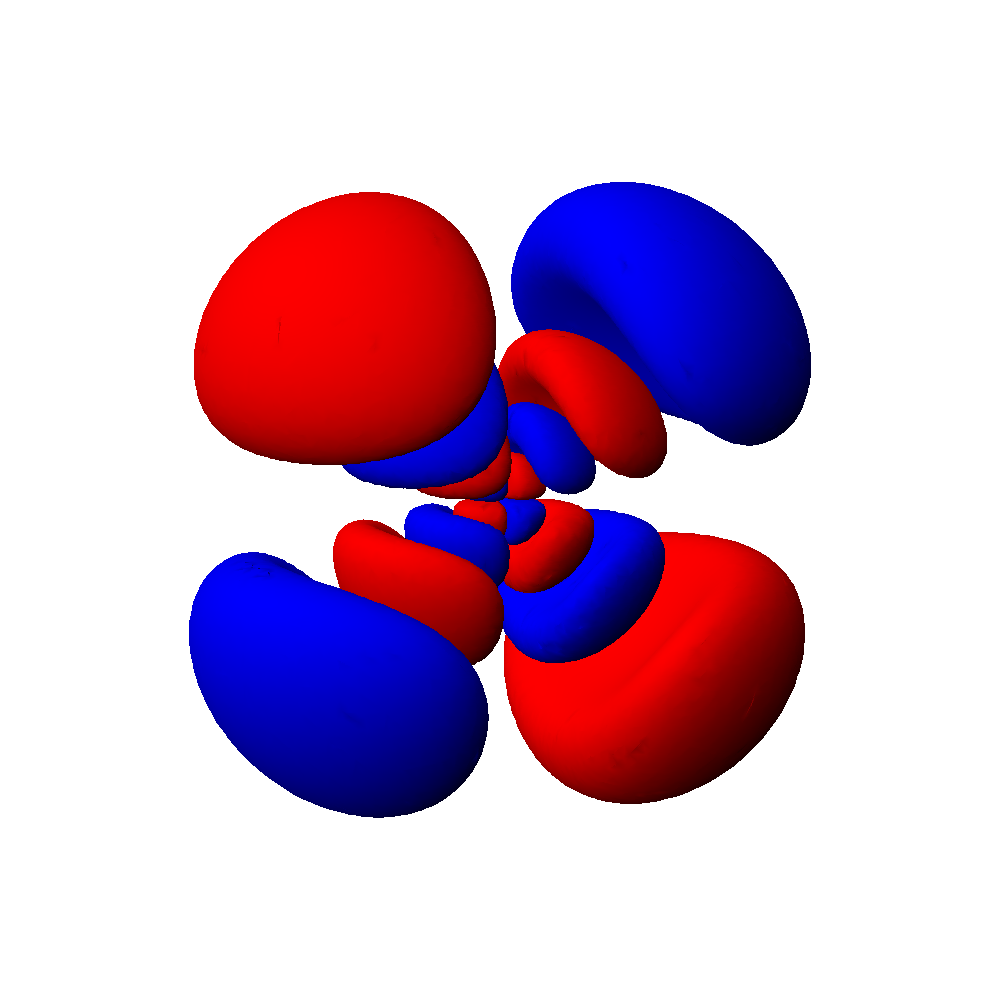
\includegraphics[width=1.6cm]{tableau_geometrie_orbitale_modelisation/D6xz.png}  
&
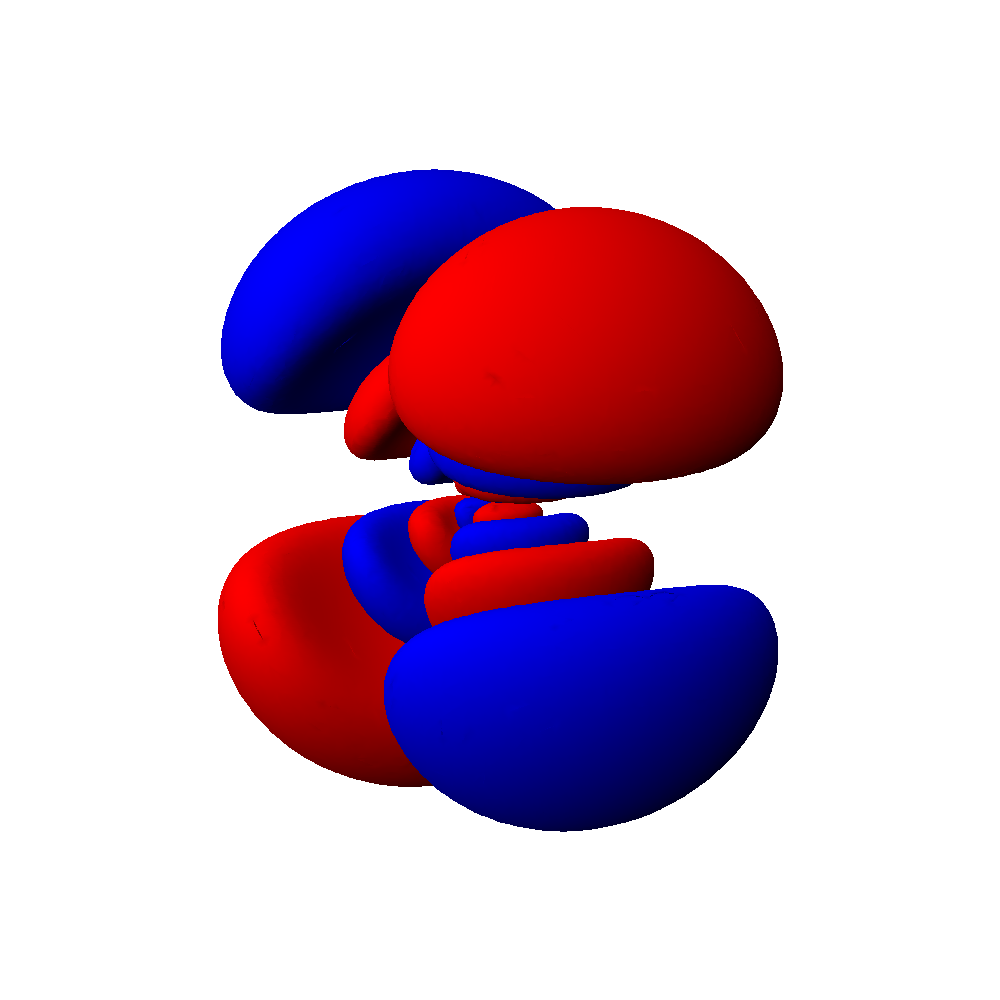
\includegraphics[width=1.6cm]{tableau_geometrie_orbitale_modelisation/D6yz.png} 
& 
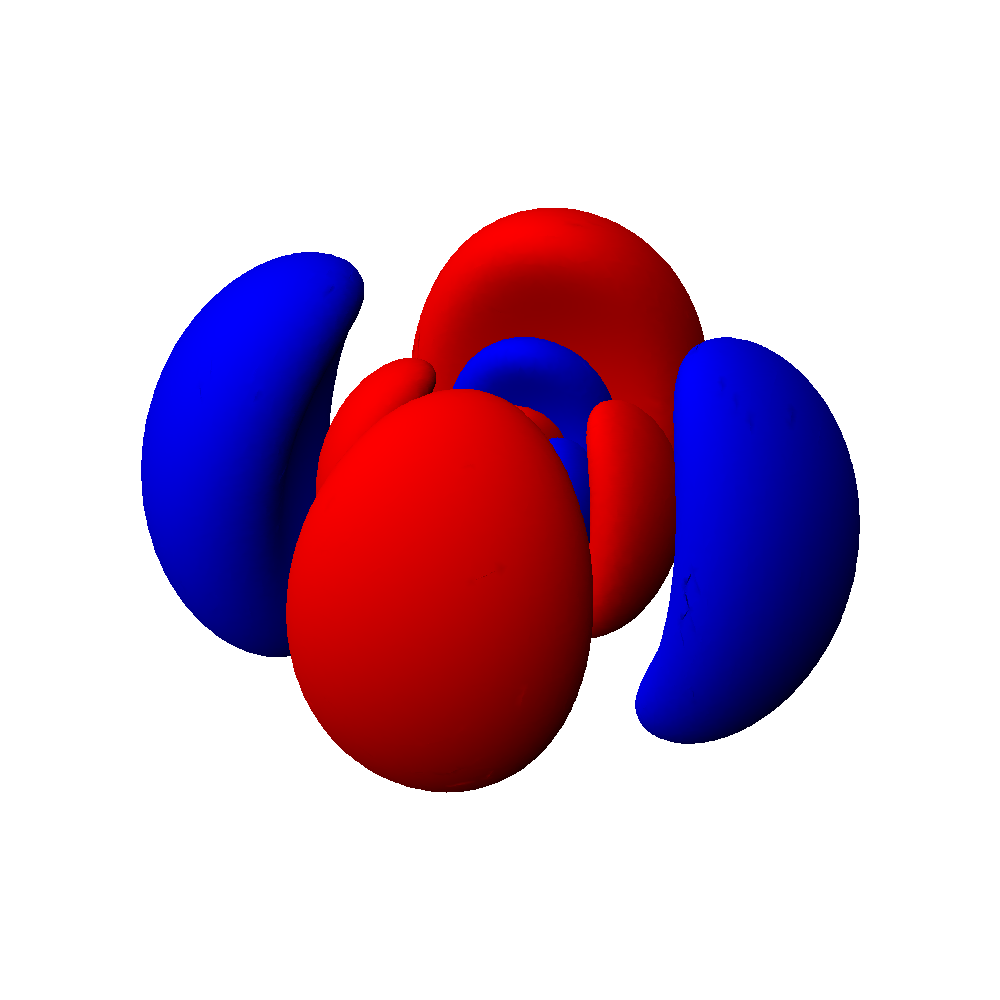
\includegraphics[width=1.6cm]{tableau_geometrie_orbitale_modelisation/D6xy.png} 
&
\includegraphics[width=1.6cm]{tableau_geometrie_orbitale_modelisation/D6x2-y2.png} 
& & \\
& & & \makecell[c]{$6d_{z^2}$} & \makecell[c]{$6d_{xz}$} & \makecell[c]{$6d_{yz}$} & \makecell[c]{$6d_{xy}$} & \makecell[c]{$6d_{x^{2}-y^{2}}$} & &  \\ %centrer la cellule individuellement 

\midrule

\multirow[t]{2}{*}{$n=7$} & \multirow[t]{2}{*}{$\ell=0$} & \multirow[t]{2}{*}{$7s$} & 
\includegraphics[width=1.6cm]{tableau_geometrie_orbitale_modelisation/S7M0.png} 
& & & & & & \\

& & & \makecell[c]{$7s$} & & & & & &  \\ %centrer la cellule individuellement 

\bottomrule

\end{xltabular}
\end{landscape}

%end{document}


\begin{figure}[!h]
		\centering
		\animategraphics[autoplay, loop, scale=0.8]{10}{fig_aluminium_modelisation_anime}{}{}
		\caption{Modélisation animée d'un atome d'aluminium avec ses différentes couches atomiques}
		\label{fig:aluminium_modelisation_animee}
\end{figure}

%\end{document}
	%--------------------------------------
%PRE-REQUIS
%--------------------------------------

%utiliser les environnement \begin{comment} \end{comment} pour mettre en commentaire le préambule une fois la programmation appelée dans le document maître (!ne pas oublier de mettre en commentaire \end{document}!)

\begin{comment}

\documentclass[a4paper, 11pt, twoside, fleqn]{memoir}

\usepackage{AOCDTF}

%--------------------------------------
%CANEVAS
%--------------------------------------

\newcommand\BoxColor{\ifcase\thechapshift blue!30\or brown!30\or pink!30\or cyan!30\or green!30\or teal!30\or purple!30\or red!30\or olive!30\or orange!30\or lime!30\or gray!\or magenta!30\else yellow!30\fi} %définition de la couleur des marqueurs de chapitre

\newcounter{chapshift} %compteur de chapitre du marqueur de chapitre
\addtocounter{chapshift}{-1}
	
\newif\ifFrame %instruction conditionnelle pour les couleurs des pages
\Frametrue

\pagestyle{plain}

% the main command; the mandatory argument sets the color of the vertical box
\newcommand\ChapFrame{%
\AddEverypageHook{%
\ifFrame
\ifthenelse{\isodd{\value{page}}}
  {\backgroundsetup{contents={%
  \begin{tikzpicture}[overlay,remember picture]
  \node[
  	rounded corners=3pt,
    fill=\BoxColor,
    inner sep=0pt,
    rectangle,
    text width=1.5cm,
    text height=5.5cm,
    align=center,
    anchor=north west
  ] 
  at ($ (current page.north west) + (-0cm,-2*\thechapshift cm) $) %nombre négatif = espacement des marqueurs entre les différents chapitres (à régler en fin de rédaction) (4.5cm vaut un espacement équivalement à la hauteur du marqueur, une page peut en contenir 6 avec cet espacement-la mais il est le plus équilibré)
    {\rotatebox{90}{\hspace*{.5cm}%
      \parbox[c][1.2cm][t]{5cm}{%
        \raggedright\textcolor{black}{\sffamily\textbf{\leftmark}}}}};
  \end{tikzpicture}}}
  }
  {\backgroundsetup{contents={%
  \begin{tikzpicture}[overlay,remember picture]
  \node[
  	rounded corners=3pt,
    fill=\BoxColor,
    inner sep=0pt,
    rectangle,
    text width=1.5cm,
    text height=5.5cm,
    align=center,
    anchor=north east
  ] 
  at ($ (current page.north east) + (-0cm,-2*\thechapshift cm) $) %nombre négatif = espacement des marqueurs entre les différents chapitres (à régler en fin de rédaction) (4.5cm vaut un espacement équivalement à la hauteur du marqueur, une page peut en contenir 6 avec cet espacement-la mais il est le plus équilibré)
    {\rotatebox{90}{\hspace*{.5cm}%
      \parbox[c][1.2cm][t]{5cm}{%
        \raggedright\textcolor{black}{\sffamily\textbf{\leftmark}}}}};
  \end{tikzpicture}}}%
  }
  \BgMaterial%
  \fi%
}%
  \stepcounter{chapshift}
}

\renewcommand\chaptermark[1]{\markboth{\thechapter.~#1}{}} %redéfinition du marqueur de chapitre pour ne contenir que le titre du chapitre %à personnaliser selon le nombre de chapitre dans le cours

%--------------------------------------
%corps du document
%--------------------------------------

\begin{document} %corps du document
	\openleft %début de chapitre à gauche

\end{comment}

\chapter{Unité de mesure et grandeurs physique}

\section{Généralités}

\subsection{Différences}

Cette annexe énumère les unités de mesures et de leur grandeurs physiques associées à connaître pour la maitrise des formules mathématiques en électrotechnique. Il convient de bien identifier ce qu'est une grandeur physique et une unité de mesure :
\begin{description}
\item[Unité de mesure] \'Etalon de mesure nécessaire pour la mesure d'une grandeur physique dont le fondement est l'exacte reproductibilité expérimentale de l'étalon\,;
\item[Grandeur physique] Toute propriété des sciences de la nature qui peut être mesurée ou calculées et dont les différentes valeurs s'expriment à l'aide d'une nombre réel ou complexe. Une grandeur physique peut s'exprimer sans unité de mesure, ce sont des \emph{grandeurs sans dimension}. Mais l'inverse n'est pas vraie, toute unité de mesure est associée une grandeur physique.\\
La notion générale de grandeur physique peut être divisées en des notions plus précises, indiquée au moyen d'indices ou d'un symbole usuel différent.
\item[Dimension] Expression de la dépendance d'une grandeur par rapport aux grandeurs de base d'un système de grandeurs sous la forme d'un produit de puissance de facteurs correspondant aux grandeurs de base, en omettant tout facteur numérique.
\end{description}
Les tableaux situés en \superref{subsec:systeme_international} sont issus des normes ISO 80000-xx\supercite{ISO:80000-2013}, les normes internationales régissant le Système International de grandeurs (\emph{International System of Quantities}, ISQ), qui font également le lien avec le Système International d'unités (SI).

\subsection{Quelques règles de rédaction}

\begin{description}
	\item[Symboles des grandeurs] Les symboles usuels des grandeurs prennent généralement la forme d'une seule lettre (alphabet grec ou latin), toujours en italique, et peuvent être précisés par des indices.
	\item [Indice] Un indice permet de différencier des grandeurs présentant le même symbole usuel ou, pour une même grandeur, différentes applications de celle-ci.
		\begin{itemize}
			\item Symbole d'une grandeur physique ou d'une variable mathématique\,;
			\item Mots ou nombres fixes.
		\end{itemize}
	\item[Symboles des unités] Les symboles des unités prennent généralement la forme d'une seule lettre (alphabet grec ou latin), toujours en caractère droit, ce qui permet de les différencier des symboles des grandeurs.\\
Une unité composée d'une multiplication de deux unités ou plus peut être indiquée de deux manières :
		\begin{gather*}
			\newton\cdot\metre \\ 
			\newton\metre
		\end{gather*}
Il convient de faire attention lorsque le symbole d'une unité est le même que celui d'un préfixe.
\end{description}

\subsection{Terminologie}

\begin{description}
\item[Coefficient] Dans une équation type $A=k \cdot B$, $k$ est le coefficient/facteur et $A$ est une grandeur proportionnelle à $B$. Usage du terme \emph{coefficient} (ou \emph{module}) lorsque les grandeurs $A$ et $B$ présentent des \emph{dimensions} différentes.
\item[Facteur] Dans une équation type $A=k \cdot B$, $k$ est le coefficient/facteur et $A$ est une grandeur proportionnelle à $B$. Usage du terme \emph{facteur} lorsque les grandeurs $A$ et $B$ sont de même \emph{dimension}.
\item[Paramètre] Combinaison de grandeurs qui apparaissent sous une telle forme dans les équations, pouvant être considérée comme constituant de nouvelles grandeurs.
\item[Nombre] Combinaison de grandeurs sans dimension.
\item[Rapport] Quotient sans dimension de deux grandeurs.
\item[Constante] Grandeur qui présente la même valeur en toutes circonstances.
\item[Massique] Adjectif apposé à une grandeur caractérisant le quotient de cette grandeur par la masse.
\item[Volumique] Adjectif apposé à une grandeur caractérisant le quotient de cette grandeur par le volume.
\item[Surfacique] Adjectif apposé à une grandeur caractérisant le quotient de cette grandeur par l'aire.
\item[Densité] Adjectif apposé à une grandeur exprimant un flux ou un courant, qui caractérise le quotient de cette grandeur par l'aire.
\item[Linéique] Adjectif apposé à une grandeur caractérisant le quotient de cette grandeur par la longueur.
\item[Molaire] Adjectif apposé à une grandeur caractérisant le quotient de cette grandeur par la quantité de matière.
\item[Concentration] Adjectif apposé à une grandeur, spécifiquement dans le cas d'un mélange, caractérisant le quotient de cette grandeur par le volume total.
\end{description}

\subsection{Alphabet}

\begin{table}[h!]
\caption{Alphabet grec}
\begin{tabularx}{\textwidth}[t]{l C C C C l C C C C}
\cmidrule[\heavyrulewidth](lr){1-5} \cmidrule[\heavyrulewidth](lr){6-10}
\thead{Nom} 		& \multicolumn{2}{c}{\thead{Caractère\\romain}} 	& \multicolumn{2}{c}{\thead{Caractère\\italique}} & \thead{Nom} 		& \multicolumn{2}{c}{\thead{Caractère\\romain}} 	& \multicolumn{2}{c}{\thead{Caractère\\italique}} \\
\cmidrule[\lightrulewidth](lr){1-5} \cmidrule[\lightrulewidth](lr){6-10}
alpha 					& A						& $\alphaup$											& \textit{A}							& $\alpha$							& nu							& N						& $\nuup$												& \textit{N}							& $\nu$ \\
beta 						& B						& $\betaup$											& \textit{B}							& $\beta$  							& xi							& $\Xiup$				& $\xiup$												& $\mathit{\Xi}$					& $\xi$ \\
gamma 				& $\Gammaup$		& $\gammaup$										& $\mathit{\Gamma}$			& $\gamma$ 							& omicron					& O						& o														& \textit{O}							& \textit{o} \\
delta						& $\Deltaup$			& $\deltaup$											& $\mathit{\Delta}$				& $\delta$ 							& pi							& $\Piup$				& $\piup$, $\varpiup$								& $\mathit{\Pi}$					& $\pi$, $\varpi$ \\
epsilon					& E						& $\epsilonup$, $\varepsilonup$				& \textit{E}							& $\epsilon$, $\varepsilon$ 	& rhô						& P						& $\rhoup$, $\varrhoup$						& \textit{P}							& $\rho$, $\varrho$ \\
zêta						& Z						& $\zetaup$											& \textit{Z}							& $\zeta$ 								& sigma					& $\Sigmaup$		& $\sigmaup$										& $\mathit{\Sigma}$				& $\sigma$ \\
êta						& H						& $\etaup$											& \textit{H}							& $\eta$								& tau						& T						& $\tauup$											& \textit{T}							& $\tau$ \\
thêta						& $\Thetaup$		& $\thetaup$, $\varthetaup$					& $\mathit{\Theta}$				& $\theta$, $\vartheta$	 		& upsilon					& Y						& $\upsilonup$										& \textit{Y}							& $\upsilon$ \\
iota						& I						& $\iotaup$											& \textit{I}							& $\iota$ 								& phi						& $\Phiup$			& $\phiup$											& $\mathit{\Phi}$					& $\phi$ \\
kappa					& K						& $\kappaup$, $\varkappaup$				& \textit{K}							& $\kappa$, $\varkappa$ 		& khi						& X						& $\chiup$												& \textit{X}							& $\chi$ \\
lambda					& $\Lambdaup$		& $\lambdaup$										& $\mathit{\Lambda}$			& $\lambda$							& psi						& $\Psiup$				& $\psiup$												& $\mathit{\Psi}$					& $\psi$ \\
mu						& M						& $\muup$											& \textit{M}							& $\mu$								& oméga					& $\Omegaup$		& $\omegaup$										& $\mathit{\Omega}$			& $\Omega$ \\
\cmidrule[\heavyrulewidth](lr){1-5} \cmidrule[\heavyrulewidth](lr){6-10}
\end{tabularx}
\end{table}


\subsection{Système International}
\label{subsec:systeme_international}

\subsubsection{Généralités}

Le Système International d'unités est un système cohérent d'unités dans l'\emph{ISQ}. Il est abrégé \emph{SI} dans toutes les langues et est formé de :
\begin{itemize}
\item Sept unités de base\,;
\item Des unités dérivées de ces unités de base.
\end{itemize}

\subsubsection{Unités SI et grandeurs}

\begin{table}[!h]
\caption{Unités SI et grandeurs correspondante de base\label{tab:unites_SI_base}}
\begin{tabularx}{\textwidth}{X R X R}
\toprule
\multicolumn{2}{c}{\thead{Grandeur de base de l'ISQ}} & \multicolumn{2}{c}{\thead{Unité SI de base}} \\
\cmidrule(lr){1-2} \cmidrule(lr){3-4} 
\thead[l]{Nom} & \thead[r]{Symbole usuel} & \thead[l]{Nom} & \thead[r]{Symbole} \\
\midrule 
Longueur 									& $L$ 			& mètre 			& \meter \\
Masse										& $M, m$ 		& kilogramme 	& \kilogram \\
Temps										& $T$			& seconde			& \second \\
Courant électrique 					& $I$				& ampère			& \ampere \\
Température thermodynamique	& $\Theta$	& kelvin				& \kelvin \\
Quantité de matière					& $N$			& mole				& \mole \\
Intensité lumineuse					& $J$				& candela			& \candela \\
\bottomrule
\end{tabularx}
\end{table}

\begin{table}[!h]
\caption{Préfixes des unités SI \label{tab:prefixes_unites_SI}}
\begin{tabularx}{\textwidth}{C X r C X r}
\cmidrule[\heavyrulewidth](lr){1-3} \cmidrule[\heavyrulewidth](lr){4-6} 

\multirow[c]{2}{*}{\thead{Facteur}} 	& \multicolumn{2}{c}{\thead{Préfixe}} 	& \multirow[c]{2}{*}{\thead{Facteur}} 	& \multicolumn{2}{c}{\thead{Préfixe}} \\

\cmidrule(lr){2-3} \cmidrule(lr){5-6} 

															& \thead[l]{Nom} 		& \thead[r]{Symbole}	& 									& \thead[l]{Nom} 		& \thead[r]{Symbole} \\
\cmidrule[\lightrulewidth](lr){1-3} \cmidrule[\lightrulewidth](lr){4-6} 
$10^{24}$											& yotta 						& Y		& $10^{-1}$											& déci 						& d  \\
$10^{21}$											& zetta 						& Z  		& $10^{-2}$											& centi 						& c  \\ 
$10^{18}$											& exa 						& E  		&															&								&	\\ 
$10^{15}$											& péta 						& P  		& $10^{-3}$											& milli 						& m  \\ 
															&								&			& $10^{-6}$											& micro 					& $\mu$  \\ 
$10^{12}$											& téra 						& T  		& $10^{-9}$											& nano 						& n  \\
$10^{9}$												& giga 						& G  		& $10^{-12}$										& pico 						& p  \\
$10^{6}$												& méga 					& M  		& 															&								& \\
$10^{3}$												& kilo 						& k 		& $10^{-15}$										& femto 					& f  \\
															&								&			& $10^{-18}$										& atto 						& a  \\
$10^{2}$												& hecto 					& h		& $10^{-21}$										& zepto 					& z \\
$10^{1}$												& déca	 					& da 		& $10^{-24}$										& yocto	 					& y \\
\cmidrule[\heavyrulewidth](lr){1-3} \cmidrule[\heavyrulewidth](lr){4-6} 
\end{tabularx}
\end{table}

\begin{xltabular}{\textwidth}{X r X O}
\caption{Unités SI dérivées avec des noms et des symboles spéciaux\label{tab:unites_SI_derivee}}\\
\toprule
\multicolumn{2}{c}{\thead{Grandeur dérivée de l'ISQ}} & \multicolumn{3}{c}{\thead{Unité SI dérivée}} \\
\cmidrule(lr){1-2} \cmidrule(lr){3-5}
\thead[l]{Nom} & \thead[r]{Symbole usuel} & \thead[l]{Nom} & \multicolumn{2}{c}{\thead[c]{Symbole \& Valeur}} \\
\midrule %filet de milieu de tableau
\endfirsthead %en-tête de la première page du tableau  
\multicolumn{5}{l}{\small\textit{Page précédente}} \\
\midrule %filet de milieu de tableau
\multicolumn{2}{c}{\thead{Grandeur dérivée de l'ISQ}} & \multicolumn{3}{c}{\thead{Unité SI dérivée}} \\
\cmidrule(lr){1-2} \cmidrule(lr){3-5}
\thead[l]{Nom} & \thead[r]{Symbole usuel} & \thead[l]{Nom} & \multicolumn{2}{l}{\thead[l]{Symbole \& Valeur}} \\
\midrule %filet de milieu de tableau
\endhead %en-tête de la première page du tableau  
\midrule %filet de milieu de tableau
\multicolumn{5}{r}{\small\textit{Page suivante}} \\
\endfoot %pied de page de toutes les pages du tableau
\bottomrule
\endlastfoot %pied de page de la dernièredu tableau
Angle plan											& $\alpha$ 						& radian 			& \radian 					& \si{\meter\per\meter} \\
Angle solide										& $\Omega$						& stéradian	 	&	\steradian		 		& 	\si{\square\meter\per\square\meter} \\
Fréquence 										& $f$									& hertz				&	\hertz 					&	\si{\per\second} \\
Force												& $F$								& newton			&	\newton					&  \si{\kilogram\meter\per\square\second} \\
Pression, contrainte							& $P$								& pascal			&	\pascal					& 	\si{\newton\per\square\meter} \\
\'Energie, travail								& $W$								& joule				& 	\joule					& 	\si{\kilo\gram\square\meter\per\square\second} \\
Puissance											& $P$								& watt				& 	\watt						&	\si{\joule\per\second} \\
Charge électrique								& $Q$								& coulomb			& 	\coulomb				&	\si{\ampere\second} \\
Différence de potentiel électrique		& $U, V$							& volt				& 	\volt						&	\si{\watt\per\ampere} \\
Capacité électrique							& $C$								& farad				& 	\farad					& \si{\coulomb\per\volt} \\
Résistance électrique							& $R$								& ohm				& 	\ohm						& \si{\volt\per\ampere} \\
Conductance électrique						& $G$								& siemens			&	\siemens				& \si{\per\ohm} \\
Flux magnétique								& $\Phi$							& weber			&	\weber					& \si{\volt\second} \\
Induction magnétique						& $\overrightarrow{B}$		& tesla				& \tesla						& \si{\weber\per\square\meter} \\
Inductance										& $L$								& henry				& \henry					& \si{\weber\per\ampere} \\
Température Celsius							& $T$								& celsius			& \celsius					& \kelvin - 273,15 \\
Flux lumineux									& $J$									& lumen			& \lumen					& \si{\candela\steradian} \\
\'Eclairement lumineux						& $E, E_v$							& lux					& \lux						& \si{\lumen\per\square\meter} \\
\end{xltabular}

\begin{table}[!h]
\caption{Unités en usage avec le SI\label{tab:unites_usage_SI}}
\begin{tabularx}{\textwidth}{X r X O}
\toprule
\multicolumn{2}{c}{\thead{Grandeur}} & \multicolumn{3}{c}{\thead{Unités}} \\
\cmidrule(lr){1-2} \cmidrule(lr){3-5} 
\thead[l]{Nom} & \thead[r]{Symbole usuel} & \thead[l]{Nom} & \multicolumn{2}{l}{\thead[l]{Symbole \& Valeur}} \\
\midrule
Temps											& $t$								 	& minute 			& \minute 				& \SI{60}{\second} \\
													& 											& heure				& \hour					& \SI{60}{\minute} \\
													&											&	jour				& \si{\day}			& \SI{24}{\hour} \\
\addlinespace
Angle plan										& $\alpha$							& degré				& \degree				& \sfrac{180}{\pi}\times\radian \\
													&											& minute			& \arcminute			& \sfrac{1}{60}\times\degree \\
													&											& seconde			& \arcsecond			& \sfrac{1}{60}\times\arcminute \\
\addlinespace
Volume											& $V$									& litre				& \litre, \liter			& \si{\cubic\deci\metre} \\
\addlinespace
Masse											& $M, m$								& tonne				& \tonne				& \SI{1000}{\kilo\gram} \\
\bottomrule
\end{tabularx}
\end{table}

\begin{table}[H]
\caption{Unités en usage avec le SI dont la valeur est obtenue expérimentalement\label{tab:unites_SI_experimentales}}
\begin{tabularx}{\textwidth}{X r X O}
\toprule
\multicolumn{2}{c}{\thead{Grandeur}} 		& \multicolumn{3}{c}{\thead{Unités}} \\
\cmidrule(lr){1-2} \cmidrule(lr){3-5} 
\thead[l]{Nom} & \thead[r]{Symbole\\usuel} 	& \thead[l]{Nom} 	& \multicolumn{2}{c}{\thead[c]{Symbole \& Valeur}} \\
\midrule
\'Energie 		& $W$ 			& électronvolt 					& \multicolumn{2}{p{8cm}}{\'Energie cinétique acquise par un électron en traversant une différence de potentiel de 1v dans le vide.} \\%
					& 					& 										& \electronvolt					& \SI{1,602176634e-19}{\joule} \\
\addlinespace
Masse			& $M, m$		& dalton							& \multicolumn{2}{p{8cm}}{$\sfrac{1}{12}$ de la masse d'un atome du nucléide \ce{^{12}C} au repos et à l'état fondamental.} \\%
					& 					& 										& \dalton							& \SI{1,660538782e-27}{\kilo\gram} \\
\addlinespace
Longueur		& $L$			& unité astronomique			& \multicolumn{2}{p{8cm}}{Valeur conventionnelle approximativement égale à la valeur moyenne de la distance entre le Soleil et la Terre.} \\%
					& 					& 										& \astronomicalunit			& \SI{1,49597870691e11}{\metre} \\
\bottomrule
\end{tabularx}
\end{table}

\section{Mathématique}

Les tableaux suivants sont extraits de l'ouvrage \citetitle{BourgeoisCogniel2005}, ils référencent les notations mathématiques utilisées en électrotechnique.

\begin{table}[!h]
\caption{Signes mathématiques\label{tab:signes_mathematiques}}
\begin{minipage}[t]{0.49\linewidth}
\begin{tabularx}{\textwidth}[t]{j j X}
\toprule
\multicolumn{1}{c}{\thead{Signe}} 		& \multicolumn{1}{c}{\thead{Utilisation}}		& \multicolumn{1}{c}{\thead{\'Enoncé}}	\\
\midrule
=																& a=b																& $a$ égal $b$ \\	
\neq															& a\neq b															& $a$ est différent de $b$	\\
\triangleq													& a\triangleq b													& $a$ correspond à $b$	\\
\simeq														& a\simeq b														& $a$ est approximativement égal à $b$	\\
<																& a < b																& $a$ est strictement inférieur à $b$	\\
>																& a > b																& $a$ est strictement supérieur à $b$		\\
\leq															& a\leq b															& $a$ est inférieur ou égal à $b$	\\
\geq															& a\geq b															& $a$ est supérieur ou égal à $b$	\\
\ll																& a\ll b																& $a$ est très inférieur ou égal à $b$	\\
\gg															& a\gg b															& $a$ est très supérieur ou égal à $b$	\\
\addlinespace
\infty															&																		& infini	\\
\addlinespace
\pm															& a\pm b															& $a$ plus ou moins $b$	\\
\in																& x\in A																& $x$ appartient à $a$	\\
\notin														& x\notin A 														& $x$ n'appartient pas à $a$	\\
\bottomrule
\end{tabularx}
\end{minipage}
\hfill
\begin{minipage}[t]{0.49\linewidth}
\begin{tabularx}{\textwidth}[t]{j j X}
\toprule
\multicolumn{1}{c}{\thead{Signe}} 		& \multicolumn{1}{c}{\thead{Utilisation}}		& \multicolumn{1}{c}{\thead{\'Enoncé}}	\\
\midrule
+					& a+b														& $a$ plus $b$ \\
-					& a-b															& $a$ moins $b$ \\
\addlinespace
\times			& a\times b												& $a$ multiplié par $b$ \\
\cdot				& a\cdot  b												& \\
					& a\ b														& \\
\addlinespace
\frac\				& \frac{a}{b}											& $a$ divisé par $b$ \\
/					& a/b															& \\
\addlinespace
\sum				& {\displaystyle\sum_{i=1}^{n} a_{i}} 	& $a_{1} + a_{2} + a_{3} \ldots a_{n}$ \\
\addlinespace
\prod				& {\displaystyle\prod_{i=1}^{n} a_{i}}	& $a_{1} \times a_{2} \times a_{3} \ldots a_{n}$ \\
\addlinespace
!					& n!															& $1 \times 2 \times 3 \ldots n$ \\
					& a^{n}													& $a$ puissance $n$ \\
					& \sqrt{a}													& racine carrée de $a$ \\
\addlinespace
					& \sqrt[n]{a}												& racine n\ieme de $a$ \\
					& a^{1/n}													& \\
\addlinespace
\vert\ \vert\	& \vert a \vert											& valeur absolue de $a$	\\
\bottomrule
\end{tabularx}
\end{minipage}
\end{table}


\captionof{table}{Classification des locaux}
\begin{minipage}[t]{0.49\linewidth}
\begin{tabularx}{\textwidth}[t]{i X}
\toprule
\multicolumn{1}{c}{\thead{Symbole}} 		& \multicolumn{1}{c}{\thead{\'Enoncé}} \\
\midrule
f													& fonction ou application \\
f(x)												&	valeur de la fonction $f$ respectivement en $x$ \\
\left[ f(x) \right] ^{a} _{b}				& $f(b)-f(a)$ \\
\addlinespace
f(x)\ | ^{a} _{b} 							& 	\\
\addlinespace
\lim\limits_{x \rightarrow a} f(x)		& limite de $f(x)$ quand $x$ tend vers $a$ \\
\addlinespace
f\prime											& dérivée (première) de la fonction $f$ \\
\addlinespace
f^{(k)}(x)										& dérivée d'ordre $k$ de la fonction $f$ \\
\addlinespace					
\Delta f											& dérivée totale globale de la fonction $f$\supercite{Wiki:NDS} \\
\frac{df}{dx}								& dérivée totale locale de la fonction $f$ par rapport à $x$ \\
\frac{\partial f}{\partial x}				& dérivée partielle locale de la fonction $f$ par rapport à $x$ \\
\end{tabularx}
\end{minipage}
\hfill
\begin{minipage}[t]{0.49\linewidth}
\begin{tabularx}{\textwidth}[t]{i X}
\toprule
\multicolumn{1}{c}{\thead{Symbole}} 		& \multicolumn{1}{c}{\thead{\'Enoncé}} \\
\midrule
\frac{\delta f}{\delta x}					& variation élémentaire de la fonction $f$ par rapport à $x$ \\
\int_{a}^b f(x)dx							& intégrale définie de la fonction $f$ de $a$ à $b$ \\
\int_{a}^b f(x)dx							& intégrale définie de la fonction $f$ de $a$ à $b$ \\
\addlinespace					
\mathbb{N}									& ensemble des entiers naturels \\
\mathbb{Z}									& ensemble des entiers \\
\mathbb{Q}									& ensemble des nombres rationnels \\
\mathbb{R}									& ensemble des entiers réels \\
\mathbb{C}									& ensemble des nombres complexes \\
\mathbb{P}									& ensemble des nombres premiers \\
\cos x											&	cosinus de $x$ \\
\sin x												&	sinus de $x$ \\
\tan x											&	tangente de $x$ \\
\cot x											&	cotangente de $x$ \\
\end{tabularx}
\end{minipage}

\begin{minipage}[b]{0.49\linewidth}
\begin{tabularx}{\textwidth}{R}
\midrule
\small\textit{Colonne suivante} \\
\end{tabularx}
\end{minipage}
\hfill
\begin{minipage}{0.49\linewidth}
\begin{tabularx}{\textwidth}{R}
\midrule
\small\textit{Page suivante} \\
\end{tabularx}
\end{minipage}

\begin{minipage}[t]{0.49\linewidth}
\begin{tabularx}{\textwidth}[t]{i X}
\multicolumn{1}{c}{\thead{Symbole}} 		& \multicolumn{1}{c}{\thead{\'Enoncé}} \\
\midrule
\arccos x										& réciproque du cosinus de $x$ \\
\arcsin x										& inverse du sinus de $x$ \\
\arctan x										& inverse de la tangente de $x$ \\
e = 2,7182818								& base des logarithmes népériens \\
\exp x											& exponentielle de base $e$ de $x$ \\
\midrule
\multicolumn{2}{r}{\small\textit{Colonne suivante}} \\
\end{tabularx}
\end{minipage}
\hfill
\begin{minipage}[t]{0.49\linewidth}
\begin{tabularx}{\textwidth}[t]{i X}
\multicolumn{1}{c}{\thead{Symbole}} 		& \multicolumn{1}{c}{\thead{\'Enoncé}} \\
\midrule
\ln x												& logarithme népérien de $x$ \\
\lg x 												& logarithme décimal de $x$ \\
\mathrm{i\ ou\ j}							& unité imaginaire \\
\arg 												& argument \\	
\bottomrule				
\end{tabularx}
\end{minipage}


\section{Espace \& temps}

\subsection{Généralités}

Les tableaux suivants détaillent les noms, les symboles et les définitions des unités et grandeurs utilisées pour décrire mathématiquement l'espace et le temps. Ces notations seront d'application pour le restant des cours.

\begin{xltabular}{\textwidth}{l k l k X}
\caption{Unités SI et grandeurs définissant l'espace et le temps\label{tab:unites_espace_temps}} \\
\toprule
\multicolumn{2}{c}{\thead{Grandeur}} & \multicolumn{2}{c}{\thead{Unité}} & \multirow{2}{*}{\thead[c]{Remarque}} \\
\cmidrule(lr){1-2} \cmidrule(lr){3-4}
\thead[l]{Nom} & \multicolumn{1}{r}{\thead[r]{Symbole usuel}} & \thead[l]{Nom} & \multicolumn{1}{r}{\thead[r]{Symbole}} & \\
\midrule %filet de milieu de tableau
\endfirsthead %en-tête de la première page du tableau  
\multicolumn{5}{l}{\small\textit{Page précédente}} \\
\midrule %filet de milieu de tableau
\multicolumn{2}{c}{\thead{Grandeurs}} & \multicolumn{2}{c}{\thead{Unités}} & \multirow{2}{*}{\thead[c]{Remarques}} \\
\cmidrule(lr){1-2} \cmidrule(lr){3-4}
\thead[l]{Nom} & \multicolumn{1}{r}{\thead[r]{Symbole usuel}} & \thead[l]{Nom} & \multicolumn{1}{r}{\thead[r]{Symbole}} & \\
\midrule %filet de milieu de tableau
\endhead %en-tête de la première page du tableau  
\midrule %filet de milieu de tableau
\multicolumn{5}{r}{\small\textit{Page suivante}} \\
\endfoot %pied de page de toutes les pages du tableau
\bottomrule
\endlastfoot %pied de page de la dernièredu tableau
Longueur 						& L, l					& Mètre				& \metre				& \\
Largeur							& B, b				& 						&							& \\
Hauteur							& H, h				&						&							& Le symbole $H$ est régulièrement utilisé pour désigner l'altitude. \\
\'Epaisseur					& d, \delta			& 						&							& \\
Rayon							& R, r				&						&							& \\
Distance radiale				& r_{Q}, \rho		&						&							& \\
Diamètre						& D, d				&						&							& \\
Longueur curviligne		& s					&						&							& \\
Distance						& d, r				& 						&							& \\
Rayon (vecteur)				& \mathbf{r}		&						&							& \\
\end{xltabular}

%\end{document}

	
%--------------------------------------
%conclusion, bibliographie
%--------------------------------------

\backmatter
	
	%--------------------------------------
	%inclusion des chapitres
	%--------------------------------------
	
	
	
	%--------------------------------------
	%bibliographie
	%--------------------------------------

	\nocite{Coarer2003} %appel les références utilisées pour la construction du document mais non citées (clés insensibles à la casse)
	
	\printbibliography %ajout des références bibliographiques

\end{document}
